\PassOptionsToPackage{unicode=true}{hyperref} % options for packages loaded elsewhere
\PassOptionsToPackage{hyphens}{url}
%
\documentclass[]{book}
\usepackage{lmodern}
\usepackage{amssymb,amsmath}
\usepackage{ifxetex,ifluatex}
\usepackage{fixltx2e} % provides \textsubscript
\ifnum 0\ifxetex 1\fi\ifluatex 1\fi=0 % if pdftex
  \usepackage[T1]{fontenc}
  \usepackage[utf8]{inputenc}
  \usepackage{textcomp} % provides euro and other symbols
\else % if luatex or xelatex
  \usepackage{unicode-math}
  \defaultfontfeatures{Ligatures=TeX,Scale=MatchLowercase}
\fi
% use upquote if available, for straight quotes in verbatim environments
\IfFileExists{upquote.sty}{\usepackage{upquote}}{}
% use microtype if available
\IfFileExists{microtype.sty}{%
\usepackage[]{microtype}
\UseMicrotypeSet[protrusion]{basicmath} % disable protrusion for tt fonts
}{}
\IfFileExists{parskip.sty}{%
\usepackage{parskip}
}{% else
\setlength{\parindent}{0pt}
\setlength{\parskip}{6pt plus 2pt minus 1pt}
}
\usepackage{hyperref}
\hypersetup{
            pdftitle={Supplemental Material: Base Diagnostics},
            pdfauthor={Jose Guadalupe Hernandez},
            pdfborder={0 0 0},
            breaklinks=true}
\urlstyle{same}  % don't use monospace font for urls
\usepackage[margin=1in]{geometry}
\usepackage{color}
\usepackage{fancyvrb}
\newcommand{\VerbBar}{|}
\newcommand{\VERB}{\Verb[commandchars=\\\{\}]}
\DefineVerbatimEnvironment{Highlighting}{Verbatim}{commandchars=\\\{\}}
% Add ',fontsize=\small' for more characters per line
\usepackage{framed}
\definecolor{shadecolor}{RGB}{248,248,248}
\newenvironment{Shaded}{\begin{snugshade}}{\end{snugshade}}
\newcommand{\AlertTok}[1]{\textcolor[rgb]{0.94,0.16,0.16}{#1}}
\newcommand{\AnnotationTok}[1]{\textcolor[rgb]{0.56,0.35,0.01}{\textbf{\textit{#1}}}}
\newcommand{\AttributeTok}[1]{\textcolor[rgb]{0.77,0.63,0.00}{#1}}
\newcommand{\BaseNTok}[1]{\textcolor[rgb]{0.00,0.00,0.81}{#1}}
\newcommand{\BuiltInTok}[1]{#1}
\newcommand{\CharTok}[1]{\textcolor[rgb]{0.31,0.60,0.02}{#1}}
\newcommand{\CommentTok}[1]{\textcolor[rgb]{0.56,0.35,0.01}{\textit{#1}}}
\newcommand{\CommentVarTok}[1]{\textcolor[rgb]{0.56,0.35,0.01}{\textbf{\textit{#1}}}}
\newcommand{\ConstantTok}[1]{\textcolor[rgb]{0.00,0.00,0.00}{#1}}
\newcommand{\ControlFlowTok}[1]{\textcolor[rgb]{0.13,0.29,0.53}{\textbf{#1}}}
\newcommand{\DataTypeTok}[1]{\textcolor[rgb]{0.13,0.29,0.53}{#1}}
\newcommand{\DecValTok}[1]{\textcolor[rgb]{0.00,0.00,0.81}{#1}}
\newcommand{\DocumentationTok}[1]{\textcolor[rgb]{0.56,0.35,0.01}{\textbf{\textit{#1}}}}
\newcommand{\ErrorTok}[1]{\textcolor[rgb]{0.64,0.00,0.00}{\textbf{#1}}}
\newcommand{\ExtensionTok}[1]{#1}
\newcommand{\FloatTok}[1]{\textcolor[rgb]{0.00,0.00,0.81}{#1}}
\newcommand{\FunctionTok}[1]{\textcolor[rgb]{0.00,0.00,0.00}{#1}}
\newcommand{\ImportTok}[1]{#1}
\newcommand{\InformationTok}[1]{\textcolor[rgb]{0.56,0.35,0.01}{\textbf{\textit{#1}}}}
\newcommand{\KeywordTok}[1]{\textcolor[rgb]{0.13,0.29,0.53}{\textbf{#1}}}
\newcommand{\NormalTok}[1]{#1}
\newcommand{\OperatorTok}[1]{\textcolor[rgb]{0.81,0.36,0.00}{\textbf{#1}}}
\newcommand{\OtherTok}[1]{\textcolor[rgb]{0.56,0.35,0.01}{#1}}
\newcommand{\PreprocessorTok}[1]{\textcolor[rgb]{0.56,0.35,0.01}{\textit{#1}}}
\newcommand{\RegionMarkerTok}[1]{#1}
\newcommand{\SpecialCharTok}[1]{\textcolor[rgb]{0.00,0.00,0.00}{#1}}
\newcommand{\SpecialStringTok}[1]{\textcolor[rgb]{0.31,0.60,0.02}{#1}}
\newcommand{\StringTok}[1]{\textcolor[rgb]{0.31,0.60,0.02}{#1}}
\newcommand{\VariableTok}[1]{\textcolor[rgb]{0.00,0.00,0.00}{#1}}
\newcommand{\VerbatimStringTok}[1]{\textcolor[rgb]{0.31,0.60,0.02}{#1}}
\newcommand{\WarningTok}[1]{\textcolor[rgb]{0.56,0.35,0.01}{\textbf{\textit{#1}}}}
\usepackage{longtable,booktabs}
% Fix footnotes in tables (requires footnote package)
\IfFileExists{footnote.sty}{\usepackage{footnote}\makesavenoteenv{longtable}}{}
\usepackage{graphicx,grffile}
\makeatletter
\def\maxwidth{\ifdim\Gin@nat@width>\linewidth\linewidth\else\Gin@nat@width\fi}
\def\maxheight{\ifdim\Gin@nat@height>\textheight\textheight\else\Gin@nat@height\fi}
\makeatother
% Scale images if necessary, so that they will not overflow the page
% margins by default, and it is still possible to overwrite the defaults
% using explicit options in \includegraphics[width, height, ...]{}
\setkeys{Gin}{width=\maxwidth,height=\maxheight,keepaspectratio}
\setlength{\emergencystretch}{3em}  % prevent overfull lines
\providecommand{\tightlist}{%
  \setlength{\itemsep}{0pt}\setlength{\parskip}{0pt}}
\setcounter{secnumdepth}{5}
% Redefines (sub)paragraphs to behave more like sections
\ifx\paragraph\undefined\else
\let\oldparagraph\paragraph
\renewcommand{\paragraph}[1]{\oldparagraph{#1}\mbox{}}
\fi
\ifx\subparagraph\undefined\else
\let\oldsubparagraph\subparagraph
\renewcommand{\subparagraph}[1]{\oldsubparagraph{#1}\mbox{}}
\fi

% set default figure placement to htbp
\makeatletter
\def\fps@figure{htbp}
\makeatother

\usepackage[]{natbib}
\bibliographystyle{apalike}

\title{Supplemental Material: Base Diagnostics}
\author{Jose Guadalupe Hernandez}
\date{2023-08-30}

\begin{document}
\maketitle

{
\setcounter{tocdepth}{1}
\tableofcontents
}
\hypertarget{introduction}{%
\chapter{Introduction}\label{introduction}}

This is the supplemental material for experiments with basic diagnostics.

\hypertarget{about-our-supplemental-material}{%
\section{About our supplemental material}\label{about-our-supplemental-material}}

This supplemental material is hosted on \href{https://github.com}{GitHub} using GitHub pages.
The source code and configuration files used to generate this supplemental material can be found in \href{https://github.com/jgh9094/ECJ-2023-Suite-Of-Diagnostic-Metrics-For-Characterizing-Selection-Schemes}{this GitHub repository}.
We compiled our data analyses and supplemental documentation into this nifty web-accessible book using \href{https://bookdown.org/}{bookdown}.

Our supplemental material includes the following paper figures and statistics:

\begin{itemize}
\tightlist
\item
  Exploitation rate results (Section \ref{exploitation-rate-results})
\item
  Ordered exploitation results (Section \ref{ordered-exploitation-results})
\item
  Contradictory objectives results (Section \ref{contradictory-objectives-results})
\item
  Multi-path exploration results (Section \ref{multi-path-exploration-results})
\end{itemize}

\hypertarget{contributing-authors}{%
\section{Contributing authors}\label{contributing-authors}}

\begin{itemize}
\tightlist
\item
  \href{https://jgh9094.github.io/}{Jose Guadalupe Hernandez}
\item
  \href{https://lalejini.com}{Alexander Lalejini}
\item
  \href{http://ofria.com}{Charles Ofria}
\end{itemize}

\hypertarget{computer-setup}{%
\section{Computer Setup}\label{computer-setup}}

These analyses were conducted in the following computing environment:

\begin{Shaded}
\begin{Highlighting}[]
\KeywordTok{print}\NormalTok{(version)}
\end{Highlighting}
\end{Shaded}

\begin{verbatim}
##                _                           
## platform       x86_64-pc-linux-gnu         
## arch           x86_64                      
## os             linux-gnu                   
## system         x86_64, linux-gnu           
## status                                     
## major          4                           
## minor          3.1                         
## year           2023                        
## month          06                          
## day            16                          
## svn rev        84548                       
## language       R                           
## version.string R version 4.3.1 (2023-06-16)
## nickname       Beagle Scouts
\end{verbatim}

\hypertarget{experimental-setup}{%
\section{Experimental setup}\label{experimental-setup}}

Setting up required variables variables.

\begin{Shaded}
\begin{Highlighting}[]
\CommentTok{# libraries we are using}
\KeywordTok{library}\NormalTok{(ggplot2)}
\KeywordTok{library}\NormalTok{(cowplot)}
\KeywordTok{library}\NormalTok{(dplyr)}
\end{Highlighting}
\end{Shaded}

\begin{verbatim}
## 
## Attaching package: 'dplyr'
\end{verbatim}

\begin{verbatim}
## The following objects are masked from 'package:stats':
## 
##     filter, lag
\end{verbatim}

\begin{verbatim}
## The following objects are masked from 'package:base':
## 
##     intersect, setdiff, setequal, union
\end{verbatim}

\begin{Shaded}
\begin{Highlighting}[]
\KeywordTok{library}\NormalTok{(PupillometryR)}
\end{Highlighting}
\end{Shaded}

\begin{verbatim}
## Loading required package: rlang
\end{verbatim}

\begin{Shaded}
\begin{Highlighting}[]
\CommentTok{# data diractory for gh-pages}
\NormalTok{DATA_DIR =}\StringTok{ '/opt/ECJ-2023-Suite-Of-Diagnostic-Metrics-For-Characterizing-Selection-Schemes/DATA/BASE_DIAGNOSTICS/'}

\CommentTok{# data diractory for local testing}
\CommentTok{# DATA_DIR = '~/Desktop/Repositories/ECJ-2023-Suite-Of-Diagnostic-Metrics-For-Characterizing-Selection-Schemes/DATA/BASE_DIAGNOSTICS/'}

\CommentTok{# graph variables}
\NormalTok{SHAPE =}\StringTok{ }\KeywordTok{c}\NormalTok{(}\DecValTok{5}\NormalTok{,}\DecValTok{3}\NormalTok{,}\DecValTok{1}\NormalTok{,}\DecValTok{2}\NormalTok{,}\DecValTok{6}\NormalTok{,}\DecValTok{0}\NormalTok{,}\DecValTok{4}\NormalTok{,}\DecValTok{20}\NormalTok{,}\DecValTok{1}\NormalTok{)}
\NormalTok{cb_palette <-}\StringTok{ }\KeywordTok{c}\NormalTok{(}\StringTok{'#332288'}\NormalTok{,}\StringTok{'#88CCEE'}\NormalTok{,}\StringTok{'#EE7733'}\NormalTok{,}\StringTok{'#EE3377'}\NormalTok{,}\StringTok{'#117733'}\NormalTok{,}\StringTok{'#882255'}\NormalTok{,}\StringTok{'#44AA99'}\NormalTok{,}\StringTok{'#CCBB44'}\NormalTok{, }\StringTok{'#000000'}\NormalTok{)}
\NormalTok{p_theme <-}\StringTok{ }\KeywordTok{theme}\NormalTok{(}
  \DataTypeTok{plot.title =} \KeywordTok{element_text}\NormalTok{( }\DataTypeTok{face =} \StringTok{"bold"}\NormalTok{, }\DataTypeTok{size =} \DecValTok{20}\NormalTok{, }\DataTypeTok{hjust=}\FloatTok{0.5}\NormalTok{),}
  \DataTypeTok{panel.border =} \KeywordTok{element_blank}\NormalTok{(),}
  \DataTypeTok{panel.grid.minor =} \KeywordTok{element_blank}\NormalTok{(),}
  \DataTypeTok{legend.title=}\KeywordTok{element_text}\NormalTok{(}\DataTypeTok{size=}\DecValTok{18}\NormalTok{, }\DataTypeTok{hjust =} \FloatTok{0.5}\NormalTok{),}
  \DataTypeTok{legend.text=}\KeywordTok{element_text}\NormalTok{(}\DataTypeTok{size=}\DecValTok{10}\NormalTok{),}
  \DataTypeTok{axis.title =} \KeywordTok{element_text}\NormalTok{(}\DataTypeTok{size=}\DecValTok{18}\NormalTok{),}
  \DataTypeTok{axis.text =} \KeywordTok{element_text}\NormalTok{(}\DataTypeTok{size=}\DecValTok{16}\NormalTok{),}
  \DataTypeTok{legend.position=}\StringTok{"bottom"}\NormalTok{,}
  \DataTypeTok{legend.margin =} \KeywordTok{margin}\NormalTok{(}\DecValTok{0}\NormalTok{, }\DecValTok{0}\NormalTok{, }\DecValTok{0}\NormalTok{, }\DecValTok{0}\NormalTok{),}
  \DataTypeTok{panel.background =} \KeywordTok{element_rect}\NormalTok{(}\DataTypeTok{fill =} \StringTok{"#f1f2f5"}\NormalTok{,}
                                  \DataTypeTok{colour =} \StringTok{"white"}\NormalTok{,}
                                  \DataTypeTok{linewidth =} \FloatTok{0.5}\NormalTok{, }\DataTypeTok{linetype =} \StringTok{"solid"}\NormalTok{)}
\NormalTok{)}

\CommentTok{# colors for streak plots}
\NormalTok{STK_SHAPE =}\StringTok{ }\KeywordTok{c}\NormalTok{(}\DecValTok{2}\NormalTok{,}\DecValTok{6}\NormalTok{,}\DecValTok{0}\NormalTok{,}\DecValTok{4}\NormalTok{,}\DecValTok{20}\NormalTok{,}\DecValTok{1}\NormalTok{)}
\NormalTok{stk_cb_palette <-}\StringTok{ }\KeywordTok{c}\NormalTok{(}\StringTok{'#EE3377'}\NormalTok{,}\StringTok{'#117733'}\NormalTok{,}\StringTok{'#882255'}\NormalTok{,}\StringTok{'#44AA99'}\NormalTok{,}\StringTok{'#CCBB44'}\NormalTok{, }\StringTok{'#000000'}\NormalTok{)}

\CommentTok{# default variables}
\NormalTok{DIMENSIONALITY =}\StringTok{ }\DecValTok{100}
\NormalTok{GENERATIONS =}\StringTok{ }\DecValTok{50000}

\CommentTok{# selection scheme related stuff}
\NormalTok{ACRO =}\StringTok{ }\KeywordTok{c}\NormalTok{(}\StringTok{'tru'}\NormalTok{,}\StringTok{'tor'}\NormalTok{,}\StringTok{'lex'}\NormalTok{,}\StringTok{'gfs'}\NormalTok{,}\StringTok{'pfs'}\NormalTok{,}\StringTok{'nds'}\NormalTok{,}\StringTok{'nov'}\NormalTok{,}\StringTok{'ran'}\NormalTok{)}
\NormalTok{NAMES =}\StringTok{ }\KeywordTok{c}\NormalTok{(}\StringTok{'Truncation (tru)'}\NormalTok{,}\StringTok{'Tournament (tor)'}\NormalTok{,}\StringTok{'Lexicase (lex)'}\NormalTok{, }\StringTok{'Genotypic Fitness Sharing (gfs)'}\NormalTok{,}\StringTok{'Phenotypic Fitness Sharing (pfs)'}\NormalTok{,}\StringTok{'Nondominated Sorting (nds)'}\NormalTok{,}\StringTok{'Novelty Search (nov)'}\NormalTok{,}\StringTok{'Random (ran)'}\NormalTok{)}
\end{Highlighting}
\end{Shaded}

\hypertarget{exploitation-rate-results}{%
\chapter{Exploitation rate results}\label{exploitation-rate-results}}

Here we present the results for \textbf{best performances} found by each selection scheme on the exploitation rate diagnostic.
50 replicates are conducted for each scheme explored.

\hypertarget{data-setup}{%
\section{Data setup}\label{data-setup}}

\begin{Shaded}
\begin{Highlighting}[]
\NormalTok{DIR =}\StringTok{ }\KeywordTok{paste}\NormalTok{(DATA_DIR,}\StringTok{'EXPLOITATION_RATE/'}\NormalTok{, }\DataTypeTok{sep =} \StringTok{""}\NormalTok{, }\DataTypeTok{collapse =} \OtherTok{NULL}\NormalTok{)}
\NormalTok{over_time_df <-}\StringTok{ }\KeywordTok{read.csv}\NormalTok{(}\KeywordTok{paste}\NormalTok{(DIR,}\StringTok{'over-time.csv'}\NormalTok{, }\DataTypeTok{sep =} \StringTok{""}\NormalTok{, }\DataTypeTok{collapse =} \OtherTok{NULL}\NormalTok{), }\DataTypeTok{header =} \OtherTok{TRUE}\NormalTok{, }\DataTypeTok{stringsAsFactors =} \OtherTok{FALSE}\NormalTok{)}
\NormalTok{over_time_df}\OperatorTok{$}\NormalTok{scheme <-}\StringTok{ }\KeywordTok{factor}\NormalTok{(over_time_df}\OperatorTok{$}\NormalTok{scheme, }\DataTypeTok{levels =}\NormalTok{ NAMES)}

\NormalTok{best_df <-}\StringTok{ }\KeywordTok{read.csv}\NormalTok{(}\KeywordTok{paste}\NormalTok{(DIR,}\StringTok{'best.csv'}\NormalTok{, }\DataTypeTok{sep =} \StringTok{""}\NormalTok{, }\DataTypeTok{collapse =} \OtherTok{NULL}\NormalTok{), }\DataTypeTok{header =} \OtherTok{TRUE}\NormalTok{, }\DataTypeTok{stringsAsFactors =} \OtherTok{FALSE}\NormalTok{)}
\NormalTok{best_df}\OperatorTok{$}\NormalTok{acro <-}\StringTok{ }\KeywordTok{factor}\NormalTok{(best_df}\OperatorTok{$}\NormalTok{acro, }\DataTypeTok{levels =}\NormalTok{ ACRO)}

\NormalTok{sati_df <-}\StringTok{ }\KeywordTok{read.csv}\NormalTok{(}\KeywordTok{paste}\NormalTok{(DIR,}\StringTok{'sol-fnd.csv'}\NormalTok{, }\DataTypeTok{sep =} \StringTok{""}\NormalTok{, }\DataTypeTok{collapse =} \OtherTok{NULL}\NormalTok{), }\DataTypeTok{header =} \OtherTok{TRUE}\NormalTok{, }\DataTypeTok{stringsAsFactors =} \OtherTok{FALSE}\NormalTok{)}
\NormalTok{sati_df}\OperatorTok{$}\NormalTok{acro <-}\StringTok{ }\KeywordTok{factor}\NormalTok{(sati_df}\OperatorTok{$}\NormalTok{acro, }\DataTypeTok{levels =}\NormalTok{ ACRO)}
\end{Highlighting}
\end{Shaded}

\hypertarget{performance-over-time}{%
\section{Performance over time}\label{performance-over-time}}

Best performance in a population over time.
Data points on the graph is the average performance across 50 replicates every 2000 generations.
Shading comes from the best and worse performance across 50 replicates.

\begin{Shaded}
\begin{Highlighting}[]
\NormalTok{lines =}\StringTok{ }\NormalTok{over_time_df }\OperatorTok
\StringTok{  }\KeywordTok{group_by}\NormalTok{(scheme, gen) }\OperatorTok
\StringTok{  }\NormalTok{dplyr}\OperatorTok{::}\KeywordTok{summarise}\NormalTok{(}
    \DataTypeTok{min =} \KeywordTok{min}\NormalTok{(pop_fit_max) }\OperatorTok{/}\StringTok{ }\NormalTok{DIMENSIONALITY,}
    \DataTypeTok{mean =} \KeywordTok{mean}\NormalTok{(pop_fit_max) }\OperatorTok{/}\StringTok{ }\NormalTok{DIMENSIONALITY,}
    \DataTypeTok{max =} \KeywordTok{max}\NormalTok{(pop_fit_max) }\OperatorTok{/}\StringTok{ }\NormalTok{DIMENSIONALITY}
\NormalTok{  )}
\end{Highlighting}
\end{Shaded}

\begin{verbatim}
## `summarise()` has grouped output by 'scheme'. You can override using the
## `.groups` argument.
\end{verbatim}

\begin{Shaded}
\begin{Highlighting}[]
\NormalTok{lines}\OperatorTok{$}\NormalTok{scheme <-}\StringTok{ }\KeywordTok{factor}\NormalTok{(lines}\OperatorTok{$}\NormalTok{scheme, }\DataTypeTok{levels =} \KeywordTok{c}\NormalTok{(}\StringTok{'Truncation (tru)'}\NormalTok{,}\StringTok{'Tournament (tor)'}\NormalTok{,}\StringTok{'Lexicase (lex)'}\NormalTok{,}\StringTok{'Random (ran)'}\NormalTok{,}\StringTok{'Genotypic Fitness Sharing (gfs)'}\NormalTok{,}\StringTok{'Phenotypic Fitness Sharing (pfs)'}\NormalTok{,}\StringTok{'Nondominated Sorting (nds)'}\NormalTok{,}\StringTok{'Novelty Search (nov)'}\NormalTok{))}

\NormalTok{over_time_plot =}\StringTok{ }\KeywordTok{ggplot}\NormalTok{(lines, }\KeywordTok{aes}\NormalTok{(}\DataTypeTok{x=}\NormalTok{gen, }\DataTypeTok{y=}\NormalTok{mean, }\DataTypeTok{group =}\NormalTok{ scheme, }\DataTypeTok{fill =}\NormalTok{ scheme, }\DataTypeTok{color =}\NormalTok{ scheme, }\DataTypeTok{shape =}\NormalTok{ scheme)) }\OperatorTok{+}
\StringTok{  }\KeywordTok{geom_ribbon}\NormalTok{(}\KeywordTok{aes}\NormalTok{(}\DataTypeTok{ymin =}\NormalTok{ min, }\DataTypeTok{ymax =}\NormalTok{ max), }\DataTypeTok{alpha =} \FloatTok{0.1}\NormalTok{) }\OperatorTok{+}
\StringTok{  }\KeywordTok{geom_line}\NormalTok{(}\DataTypeTok{size =} \FloatTok{0.5}\NormalTok{) }\OperatorTok{+}
\StringTok{  }\KeywordTok{geom_point}\NormalTok{(}\DataTypeTok{data =} \KeywordTok{filter}\NormalTok{(lines, gen }\OperatorTok\StringTok{ }\DecValTok{2000} \OperatorTok{==}\StringTok{ }\DecValTok{0} \OperatorTok{&}\StringTok{ }\NormalTok{gen }\OperatorTok{!=}\StringTok{ }\DecValTok{0}\NormalTok{), }\DataTypeTok{size =} \FloatTok{1.5}\NormalTok{, }\DataTypeTok{stroke =} \FloatTok{2.0}\NormalTok{, }\DataTypeTok{alpha =} \FloatTok{1.0}\NormalTok{) }\OperatorTok{+}
\StringTok{  }\KeywordTok{scale_y_continuous}\NormalTok{(}
    \DataTypeTok{name=}\StringTok{"Average trait score"}\NormalTok{,}
    \DataTypeTok{limits=}\KeywordTok{c}\NormalTok{(}\DecValTok{0}\NormalTok{, }\DecValTok{100}\NormalTok{),}
    \DataTypeTok{breaks=}\KeywordTok{seq}\NormalTok{(}\DecValTok{0}\NormalTok{,}\DecValTok{100}\NormalTok{, }\DecValTok{20}\NormalTok{),}
    \DataTypeTok{labels=}\KeywordTok{c}\NormalTok{(}\StringTok{"0"}\NormalTok{, }\StringTok{"20"}\NormalTok{, }\StringTok{"40"}\NormalTok{, }\StringTok{"60"}\NormalTok{, }\StringTok{"80"}\NormalTok{, }\StringTok{"100"}\NormalTok{)}
\NormalTok{  ) }\OperatorTok{+}
\StringTok{  }\KeywordTok{scale_x_continuous}\NormalTok{(}
    \DataTypeTok{name=}\StringTok{"Generations"}\NormalTok{,}
    \DataTypeTok{limits=}\KeywordTok{c}\NormalTok{(}\DecValTok{0}\NormalTok{, }\DecValTok{50000}\NormalTok{),}
    \DataTypeTok{breaks=}\KeywordTok{c}\NormalTok{(}\DecValTok{0}\NormalTok{, }\DecValTok{10000}\NormalTok{, }\DecValTok{20000}\NormalTok{, }\DecValTok{30000}\NormalTok{, }\DecValTok{40000}\NormalTok{, }\DecValTok{50000}\NormalTok{),}
    \DataTypeTok{labels=}\KeywordTok{c}\NormalTok{(}\StringTok{"0e+4"}\NormalTok{, }\StringTok{"1e+4"}\NormalTok{, }\StringTok{"2e+4"}\NormalTok{, }\StringTok{"3e+4"}\NormalTok{, }\StringTok{"4e+4"}\NormalTok{, }\StringTok{"5e+4"}\NormalTok{)}

\NormalTok{  ) }\OperatorTok{+}
\StringTok{  }\KeywordTok{scale_shape_manual}\NormalTok{(}\DataTypeTok{values=}\KeywordTok{c}\NormalTok{(}\DecValTok{5}\NormalTok{,}\DecValTok{3}\NormalTok{,}\DecValTok{1}\NormalTok{,}\DecValTok{20}\NormalTok{,}\DecValTok{2}\NormalTok{,}\DecValTok{6}\NormalTok{,}\DecValTok{0}\NormalTok{,}\DecValTok{4}\NormalTok{))}\OperatorTok{+}
\StringTok{  }\KeywordTok{scale_colour_manual}\NormalTok{(}\DataTypeTok{values =} \KeywordTok{c}\NormalTok{(}\StringTok{'#332288'}\NormalTok{,}\StringTok{'#88CCEE'}\NormalTok{,}\StringTok{'#EE7733'}\NormalTok{,}\StringTok{'#CCBB44'}\NormalTok{,}\StringTok{'#EE3377'}\NormalTok{,}\StringTok{'#117733'}\NormalTok{,}\StringTok{'#882255'}\NormalTok{,}\StringTok{'#44AA99'}\NormalTok{)) }\OperatorTok{+}
\StringTok{  }\KeywordTok{scale_fill_manual}\NormalTok{(}\DataTypeTok{values =} \KeywordTok{c}\NormalTok{(}\StringTok{'#332288'}\NormalTok{,}\StringTok{'#88CCEE'}\NormalTok{,}\StringTok{'#EE7733'}\NormalTok{,}\StringTok{'#CCBB44'}\NormalTok{,}\StringTok{'#EE3377'}\NormalTok{,}\StringTok{'#117733'}\NormalTok{,}\StringTok{'#882255'}\NormalTok{,}\StringTok{'#44AA99'}\NormalTok{)) }\OperatorTok{+}
\StringTok{  }\KeywordTok{ggtitle}\NormalTok{(}\StringTok{'Performance over time'}\NormalTok{)}\OperatorTok{+}
\StringTok{  }\NormalTok{p_theme }\OperatorTok{+}
\StringTok{  }\KeywordTok{guides}\NormalTok{(}
    \DataTypeTok{shape=}\KeywordTok{guide_legend}\NormalTok{(}\DataTypeTok{ncol=}\DecValTok{2}\NormalTok{, }\DataTypeTok{title.position =} \StringTok{"left"}\NormalTok{, }\DataTypeTok{title =} \StringTok{'Selection }\CharTok{\textbackslash{}n}\StringTok{Scheme'}\NormalTok{),}
    \DataTypeTok{color=}\KeywordTok{guide_legend}\NormalTok{(}\DataTypeTok{ncol=}\DecValTok{2}\NormalTok{, }\DataTypeTok{title.position =} \StringTok{"left"}\NormalTok{, }\DataTypeTok{title =} \StringTok{'Selection }\CharTok{\textbackslash{}n}\StringTok{Scheme'}\NormalTok{),}
    \DataTypeTok{fill=}\KeywordTok{guide_legend}\NormalTok{(}\DataTypeTok{ncol=}\DecValTok{2}\NormalTok{, }\DataTypeTok{title.position =} \StringTok{"left"}\NormalTok{, }\DataTypeTok{title =} \StringTok{'Selection }\CharTok{\textbackslash{}n}\StringTok{Scheme'}\NormalTok{)}
\NormalTok{  )}

\NormalTok{over_time_plot}
\end{Highlighting}
\end{Shaded}

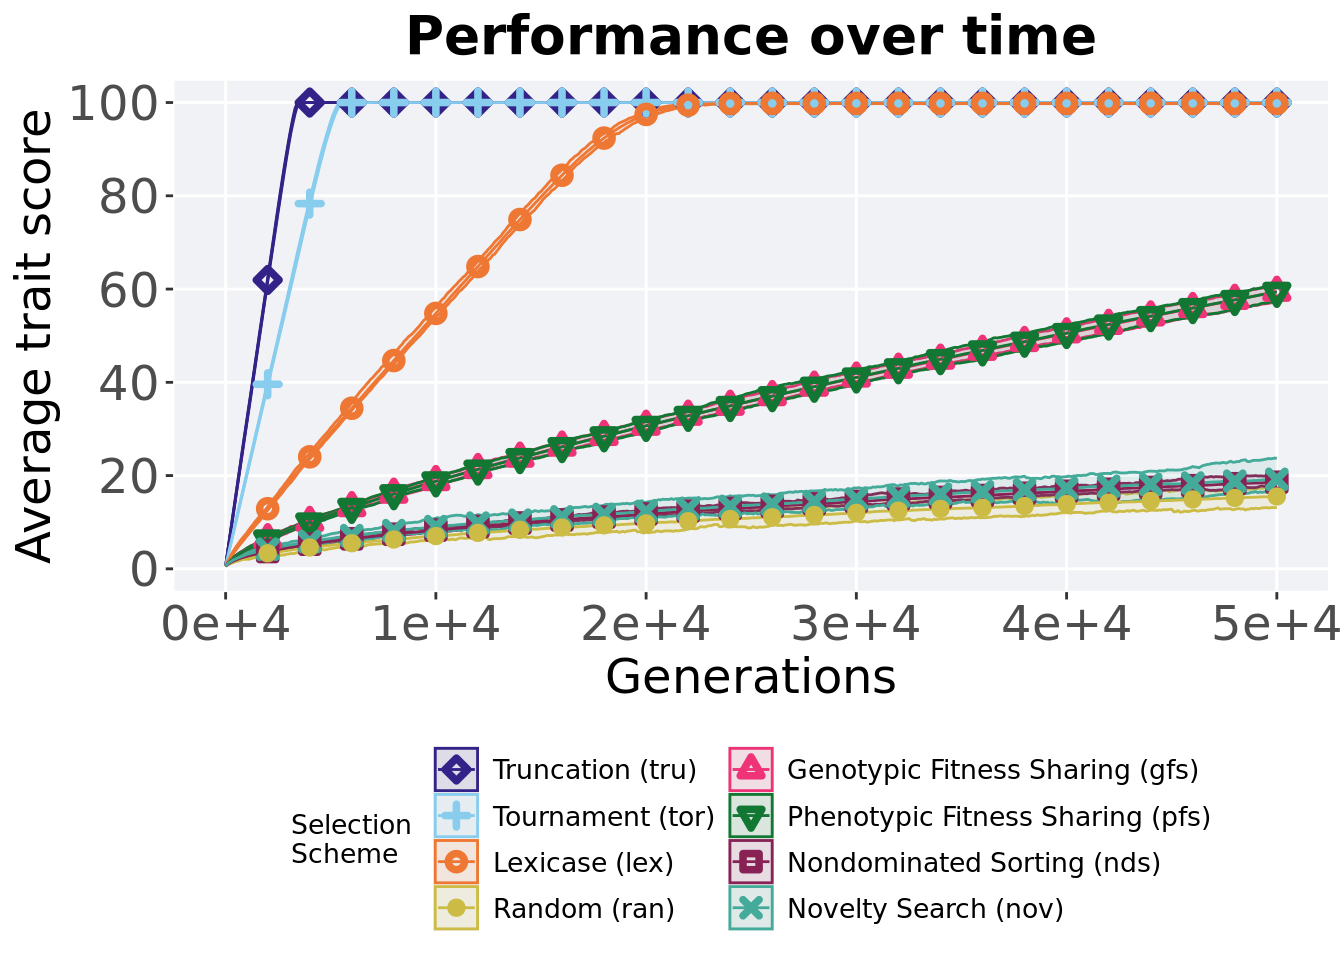
\includegraphics[width=1\linewidth]{base-diagnostics_files/figure-latex/exp-per-ot-1}

\hypertarget{best-performance-throughout}{%
\section{Best performance throughout}\label{best-performance-throughout}}

Best performance reached throughout 50,000 generations in a population.

\begin{Shaded}
\begin{Highlighting}[]
\NormalTok{plot =}\StringTok{ }\KeywordTok{filter}\NormalTok{(best_df, var }\OperatorTok{==}\StringTok{ 'pop_fit_max'}\NormalTok{) }\OperatorTok
\StringTok{  }\KeywordTok{ggplot}\NormalTok{(., }\KeywordTok{aes}\NormalTok{(}\DataTypeTok{x =}\NormalTok{ acro, }\DataTypeTok{y =}\NormalTok{ val }\OperatorTok{/}\StringTok{ }\NormalTok{DIMENSIONALITY, }\DataTypeTok{color =}\NormalTok{ acro, }\DataTypeTok{fill =}\NormalTok{ acro, }\DataTypeTok{shape =}\NormalTok{ acro)) }\OperatorTok{+}
\StringTok{  }\KeywordTok{geom_flat_violin}\NormalTok{(}\DataTypeTok{position =} \KeywordTok{position_nudge}\NormalTok{(}\DataTypeTok{x =} \FloatTok{.1}\NormalTok{, }\DataTypeTok{y =} \DecValTok{0}\NormalTok{), }\DataTypeTok{scale =} \StringTok{'width'}\NormalTok{, }\DataTypeTok{alpha =} \FloatTok{0.2}\NormalTok{, }\DataTypeTok{width =} \FloatTok{1.5}\NormalTok{) }\OperatorTok{+}
\StringTok{  }\KeywordTok{geom_boxplot}\NormalTok{(}\DataTypeTok{color =} \StringTok{'black'}\NormalTok{, }\DataTypeTok{width =} \FloatTok{.07}\NormalTok{, }\DataTypeTok{outlier.shape =} \OtherTok{NA}\NormalTok{, }\DataTypeTok{alpha =} \FloatTok{0.0}\NormalTok{, }\DataTypeTok{size =} \FloatTok{1.0}\NormalTok{, }\DataTypeTok{position =} \KeywordTok{position_nudge}\NormalTok{(}\DataTypeTok{x =} \FloatTok{.16}\NormalTok{, }\DataTypeTok{y =} \DecValTok{0}\NormalTok{)) }\OperatorTok{+}
\StringTok{  }\KeywordTok{geom_point}\NormalTok{(}\DataTypeTok{position =} \KeywordTok{position_jitter}\NormalTok{(}\DataTypeTok{width =} \FloatTok{0.03}\NormalTok{, }\DataTypeTok{height =} \FloatTok{0.02}\NormalTok{), }\DataTypeTok{size =} \FloatTok{2.0}\NormalTok{, }\DataTypeTok{alpha =} \FloatTok{1.0}\NormalTok{) }\OperatorTok{+}
\StringTok{  }\KeywordTok{scale_y_continuous}\NormalTok{(}
    \DataTypeTok{name=}\StringTok{"Average trait score"}\NormalTok{,}
    \DataTypeTok{limits=}\KeywordTok{c}\NormalTok{(}\DecValTok{0}\NormalTok{, }\FloatTok{100.1}\NormalTok{),}
    \DataTypeTok{breaks=}\KeywordTok{seq}\NormalTok{(}\DecValTok{0}\NormalTok{,}\DecValTok{100}\NormalTok{, }\DecValTok{20}\NormalTok{),}
    \DataTypeTok{labels=}\KeywordTok{c}\NormalTok{(}\StringTok{"0"}\NormalTok{, }\StringTok{"20"}\NormalTok{, }\StringTok{"40"}\NormalTok{, }\StringTok{"60"}\NormalTok{, }\StringTok{"80"}\NormalTok{, }\StringTok{"100"}\NormalTok{)}
\NormalTok{  ) }\OperatorTok{+}
\StringTok{  }\KeywordTok{scale_x_discrete}\NormalTok{(}
    \DataTypeTok{name=}\StringTok{"Scheme"}
\NormalTok{  )}\OperatorTok{+}
\StringTok{  }\KeywordTok{scale_shape_manual}\NormalTok{(}\DataTypeTok{values=}\NormalTok{SHAPE)}\OperatorTok{+}
\StringTok{  }\KeywordTok{scale_colour_manual}\NormalTok{(}\DataTypeTok{values =}\NormalTok{ cb_palette, ) }\OperatorTok{+}
\StringTok{  }\KeywordTok{scale_fill_manual}\NormalTok{(}\DataTypeTok{values =}\NormalTok{ cb_palette) }\OperatorTok{+}
\StringTok{  }\KeywordTok{ggtitle}\NormalTok{(}\StringTok{'Best performance throughout'}\NormalTok{)}\OperatorTok{+}
\StringTok{  }\NormalTok{p_theme}

\KeywordTok{plot_grid}\NormalTok{(}
\NormalTok{  plot }\OperatorTok{+}
\StringTok{    }\KeywordTok{theme}\NormalTok{(}\DataTypeTok{legend.position=}\StringTok{"none"}\NormalTok{),}
\NormalTok{  legend,}
  \DataTypeTok{nrow=}\DecValTok{2}\NormalTok{,}
  \DataTypeTok{rel_heights =} \KeywordTok{c}\NormalTok{(}\DecValTok{3}\NormalTok{,}\DecValTok{1}\NormalTok{)}
\NormalTok{)}
\end{Highlighting}
\end{Shaded}

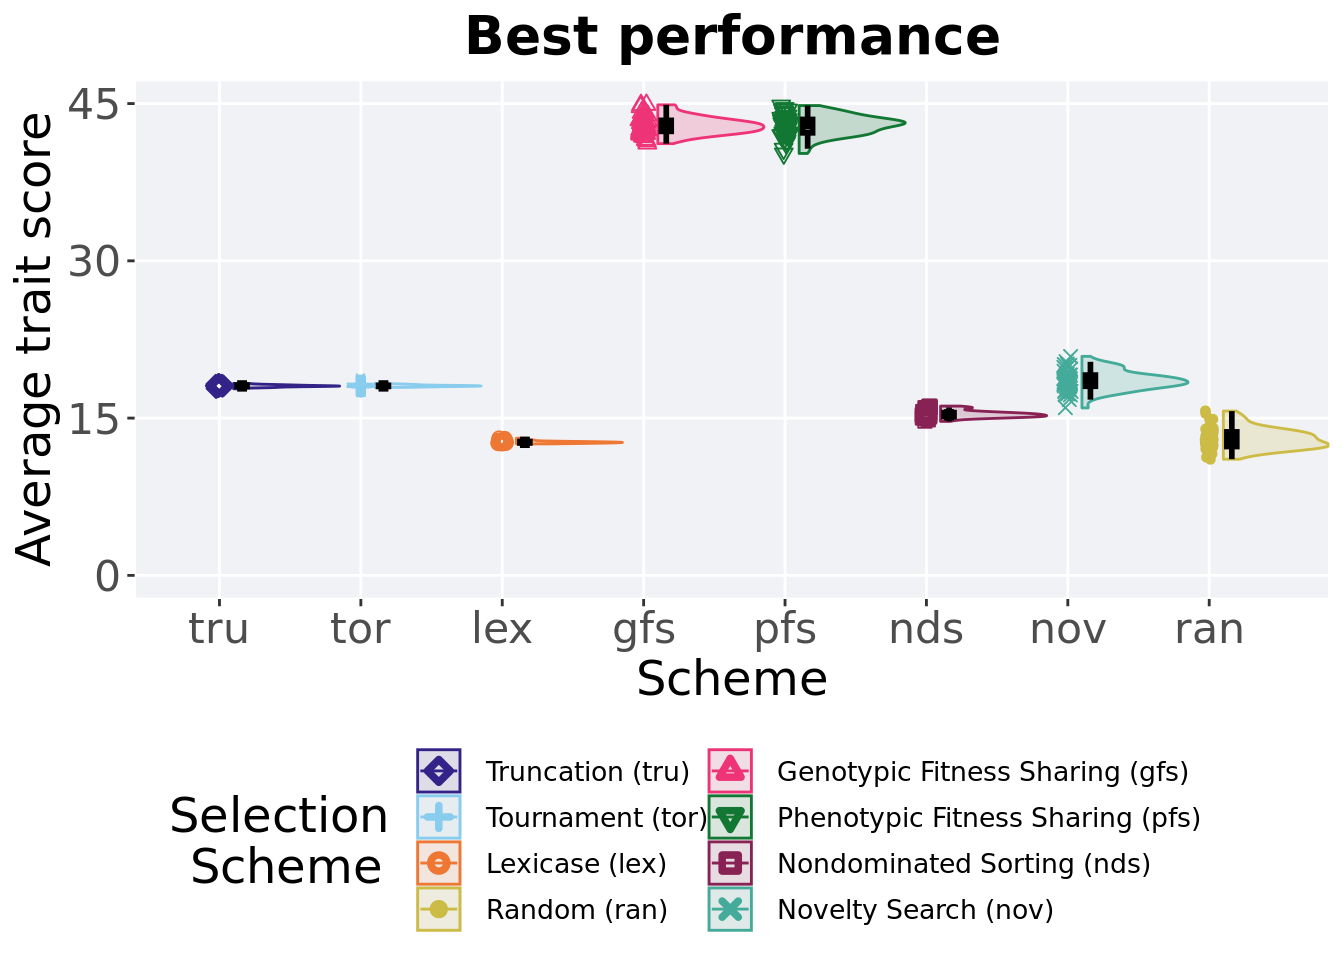
\includegraphics[width=1\linewidth]{base-diagnostics_files/figure-latex/exp-per-bst-1}

\hypertarget{stats}{%
\subsection{Stats}\label{stats}}

Summary statistics for the best performance.

\begin{Shaded}
\begin{Highlighting}[]
\NormalTok{performance =}\StringTok{ }\KeywordTok{filter}\NormalTok{(best_df, var }\OperatorTok{==}\StringTok{ 'pop_fit_max'}\NormalTok{)}
\NormalTok{performance}\OperatorTok{$}\NormalTok{acro =}\StringTok{ }\KeywordTok{factor}\NormalTok{(performance}\OperatorTok{$}\NormalTok{acro, }\DataTypeTok{levels =} \KeywordTok{c}\NormalTok{(}\StringTok{'tru'}\NormalTok{,}\StringTok{'tor'}\NormalTok{,}\StringTok{'lex'}\NormalTok{,}\StringTok{'gfs'}\NormalTok{,}\StringTok{'pfs'}\NormalTok{,}\StringTok{'nov'}\NormalTok{,}\StringTok{'nds'}\NormalTok{,}\StringTok{'ran'}\NormalTok{))}
\NormalTok{performance }\OperatorTok
\StringTok{  }\KeywordTok{group_by}\NormalTok{(acro) }\OperatorTok
\StringTok{  }\NormalTok{dplyr}\OperatorTok{::}\KeywordTok{summarise}\NormalTok{(}
    \DataTypeTok{count =} \KeywordTok{n}\NormalTok{(),}
    \DataTypeTok{na_cnt =} \KeywordTok{sum}\NormalTok{(}\KeywordTok{is.na}\NormalTok{(val)),}
    \DataTypeTok{min =} \KeywordTok{min}\NormalTok{(val }\OperatorTok{/}\StringTok{ }\NormalTok{DIMENSIONALITY, }\DataTypeTok{na.rm =} \OtherTok{TRUE}\NormalTok{),}
    \DataTypeTok{median =} \KeywordTok{median}\NormalTok{(val }\OperatorTok{/}\StringTok{ }\NormalTok{DIMENSIONALITY, }\DataTypeTok{na.rm =} \OtherTok{TRUE}\NormalTok{),}
    \DataTypeTok{mean =} \KeywordTok{mean}\NormalTok{(val }\OperatorTok{/}\StringTok{ }\NormalTok{DIMENSIONALITY, }\DataTypeTok{na.rm =} \OtherTok{TRUE}\NormalTok{),}
    \DataTypeTok{max =} \KeywordTok{max}\NormalTok{(val }\OperatorTok{/}\StringTok{ }\NormalTok{DIMENSIONALITY, }\DataTypeTok{na.rm =} \OtherTok{TRUE}\NormalTok{),}
    \DataTypeTok{IQR =} \KeywordTok{IQR}\NormalTok{(val }\OperatorTok{/}\StringTok{ }\NormalTok{DIMENSIONALITY, }\DataTypeTok{na.rm =} \OtherTok{TRUE}\NormalTok{)}
\NormalTok{  )}
\end{Highlighting}
\end{Shaded}

\begin{verbatim}
## # A tibble: 8 x 8
##   acro  count na_cnt   min median  mean   max    IQR
##   <fct> <int>  <int> <dbl>  <dbl> <dbl> <dbl>  <dbl>
## 1 tru      50      0 100    100   100   100   0     
## 2 tor      50      0 100    100   100   100   0     
## 3 lex      50      0  99.9   99.9  99.9  99.9 0.0154
## 4 gfs      50      0  57.3   59.3  59.4  61.1 0.984 
## 5 pfs      50      0  57.6   59.4  59.5  61.0 1.02  
## 6 nov      50      0  17.1   19.5  19.5  23.9 1.95  
## 7 nds      50      0  18.0   18.6  18.7  20.1 0.603 
## 8 ran      50      0  13.4   15.9  15.8  17.5 1.46
\end{verbatim}

Kruskal--Wallis test illustrates evidence of statistical differences.

\begin{Shaded}
\begin{Highlighting}[]
\KeywordTok{kruskal.test}\NormalTok{(val }\OperatorTok{~}\StringTok{ }\NormalTok{acro, }\DataTypeTok{data =}\NormalTok{ performance)}
\end{Highlighting}
\end{Shaded}

\begin{verbatim}
## 
##  Kruskal-Wallis rank sum test
## 
## data:  val by acro
## Kruskal-Wallis chi-squared = 385.26, df = 7, p-value < 2.2e-16
\end{verbatim}

Results for post-hoc Wilcoxon rank-sum test with a Bonferroni correction.

\begin{Shaded}
\begin{Highlighting}[]
\KeywordTok{pairwise.wilcox.test}\NormalTok{(}\DataTypeTok{x =}\NormalTok{ performance}\OperatorTok{$}\NormalTok{val, }\DataTypeTok{g =}\NormalTok{ performance}\OperatorTok{$}\NormalTok{acro, }\DataTypeTok{p.adjust.method =} \StringTok{"bonferroni"}\NormalTok{,}
                     \DataTypeTok{paired =} \OtherTok{FALSE}\NormalTok{, }\DataTypeTok{conf.int =} \OtherTok{FALSE}\NormalTok{, }\DataTypeTok{alternative =} \StringTok{'l'}\NormalTok{)}
\end{Highlighting}
\end{Shaded}

\begin{verbatim}
## 
##  Pairwise comparisons using Wilcoxon rank sum test with continuity correction 
## 
## data:  performance$val and performance$acro 
## 
##     tru    tor    lex    gfs    pfs    nov    nds   
## tor 1.000  -      -      -      -      -      -     
## lex <2e-16 <2e-16 -      -      -      -      -     
## gfs <2e-16 <2e-16 <2e-16 -      -      -      -     
## pfs <2e-16 <2e-16 <2e-16 1.000  -      -      -     
## nov <2e-16 <2e-16 <2e-16 <2e-16 <2e-16 -      -     
## nds <2e-16 <2e-16 <2e-16 <2e-16 <2e-16 0.018  -     
## ran <2e-16 <2e-16 <2e-16 <2e-16 <2e-16 <2e-16 <2e-16
## 
## P value adjustment method: bonferroni
\end{verbatim}

\hypertarget{generation-satisfactory-solution-found}{%
\section{Generation satisfactory solution found}\label{generation-satisfactory-solution-found}}

First generation a satisfactory solution is found throughout the 50,000 generations.

\begin{Shaded}
\begin{Highlighting}[]
\NormalTok{plot =}\StringTok{ }\NormalTok{sati_df }\OperatorTok
\StringTok{  }\KeywordTok{ggplot}\NormalTok{(., }\KeywordTok{aes}\NormalTok{(}\DataTypeTok{x =}\NormalTok{ acro, }\DataTypeTok{y =}\NormalTok{ gen , }\DataTypeTok{color =}\NormalTok{ acro, }\DataTypeTok{fill =}\NormalTok{ acro, }\DataTypeTok{shape =}\NormalTok{ acro)) }\OperatorTok{+}
\StringTok{  }\KeywordTok{geom_flat_violin}\NormalTok{(}\DataTypeTok{position =} \KeywordTok{position_nudge}\NormalTok{(}\DataTypeTok{x =} \FloatTok{.1}\NormalTok{, }\DataTypeTok{y =} \DecValTok{0}\NormalTok{), }\DataTypeTok{scale =} \StringTok{'width'}\NormalTok{, }\DataTypeTok{alpha =} \FloatTok{0.2}\NormalTok{, }\DataTypeTok{width =} \FloatTok{1.5}\NormalTok{) }\OperatorTok{+}
\StringTok{  }\KeywordTok{geom_boxplot}\NormalTok{(}\DataTypeTok{color =} \StringTok{'black'}\NormalTok{, }\DataTypeTok{width =} \FloatTok{.07}\NormalTok{, }\DataTypeTok{outlier.shape =} \OtherTok{NA}\NormalTok{, }\DataTypeTok{alpha =} \FloatTok{0.0}\NormalTok{, }\DataTypeTok{size =} \FloatTok{1.0}\NormalTok{, }\DataTypeTok{position =} \KeywordTok{position_nudge}\NormalTok{(}\DataTypeTok{x =} \FloatTok{.16}\NormalTok{, }\DataTypeTok{y =} \DecValTok{0}\NormalTok{)) }\OperatorTok{+}
\StringTok{  }\KeywordTok{geom_point}\NormalTok{(}\DataTypeTok{position =} \KeywordTok{position_jitter}\NormalTok{(}\DataTypeTok{width =} \FloatTok{0.03}\NormalTok{, }\DataTypeTok{height =} \FloatTok{0.02}\NormalTok{), }\DataTypeTok{size =} \FloatTok{2.0}\NormalTok{, }\DataTypeTok{alpha =} \FloatTok{1.0}\NormalTok{) }\OperatorTok{+}
\StringTok{  }\KeywordTok{scale_y_continuous}\NormalTok{(}
    \DataTypeTok{name=}\StringTok{"Generation"}\NormalTok{,}
    \DataTypeTok{limits=}\KeywordTok{c}\NormalTok{(}\DecValTok{0}\NormalTok{, }\DecValTok{60001}\NormalTok{),}
    \DataTypeTok{breaks=}\KeywordTok{c}\NormalTok{(}\DecValTok{0}\NormalTok{, }\DecValTok{10000}\NormalTok{, }\DecValTok{20000}\NormalTok{, }\DecValTok{30000}\NormalTok{, }\DecValTok{40000}\NormalTok{, }\DecValTok{50000}\NormalTok{, }\DecValTok{60000}\NormalTok{),}
    \DataTypeTok{labels=}\KeywordTok{c}\NormalTok{(}\StringTok{"0e+4"}\NormalTok{, }\StringTok{"1e+4"}\NormalTok{, }\StringTok{"2e+4"}\NormalTok{, }\StringTok{"3e+4"}\NormalTok{, }\StringTok{"4e+4"}\NormalTok{, }\StringTok{"5e+4"}\NormalTok{, }\StringTok{"Fail"}\NormalTok{)}
\NormalTok{  ) }\OperatorTok{+}
\StringTok{  }\KeywordTok{scale_x_discrete}\NormalTok{(}
    \DataTypeTok{name=}\StringTok{"Scheme"}
\NormalTok{  )}\OperatorTok{+}
\StringTok{  }\KeywordTok{scale_shape_manual}\NormalTok{(}\DataTypeTok{values=}\NormalTok{SHAPE)}\OperatorTok{+}
\StringTok{  }\KeywordTok{scale_colour_manual}\NormalTok{(}\DataTypeTok{values =}\NormalTok{ cb_palette, ) }\OperatorTok{+}
\StringTok{  }\KeywordTok{scale_fill_manual}\NormalTok{(}\DataTypeTok{values =}\NormalTok{ cb_palette) }\OperatorTok{+}
\StringTok{  }\KeywordTok{ggtitle}\NormalTok{(}\StringTok{'Generation satisfactory solution found'}\NormalTok{)}\OperatorTok{+}
\StringTok{  }\NormalTok{p_theme}

\KeywordTok{plot_grid}\NormalTok{(}
\NormalTok{  plot }\OperatorTok{+}
\StringTok{    }\KeywordTok{theme}\NormalTok{(}\DataTypeTok{legend.position=}\StringTok{"none"}\NormalTok{),}
\NormalTok{  legend,}
  \DataTypeTok{nrow=}\DecValTok{2}\NormalTok{,}
  \DataTypeTok{rel_heights =} \KeywordTok{c}\NormalTok{(}\DecValTok{3}\NormalTok{,}\DecValTok{1}\NormalTok{)}
\NormalTok{)}
\end{Highlighting}
\end{Shaded}

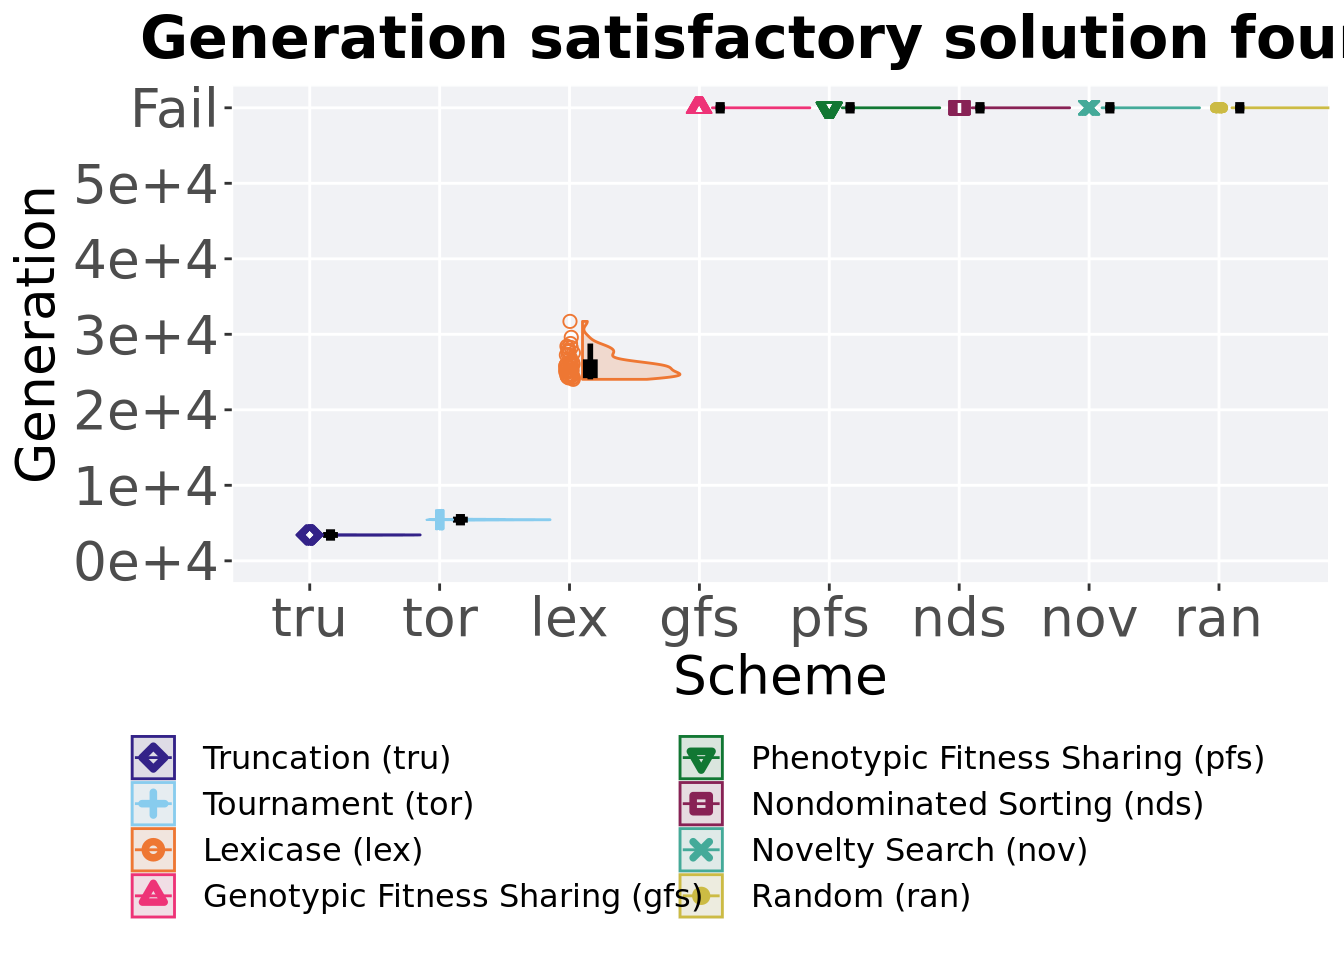
\includegraphics[width=1\linewidth]{base-diagnostics_files/figure-latex/exp-ssf-1}

\hypertarget{stats-1}{%
\subsection{Stats}\label{stats-1}}

Summary statistics for the generation a satisfactory solution is found.

\begin{Shaded}
\begin{Highlighting}[]
\NormalTok{ssf =}\StringTok{ }\KeywordTok{filter}\NormalTok{(sati_df, gen }\OperatorTok{<=}\StringTok{ }\NormalTok{GENERATIONS)}
\NormalTok{ssf}\OperatorTok{$}\NormalTok{acro =}\StringTok{ }\KeywordTok{factor}\NormalTok{(ssf}\OperatorTok{$}\NormalTok{acro, }\DataTypeTok{levels =} \KeywordTok{c}\NormalTok{(}\StringTok{'tru'}\NormalTok{,}\StringTok{'tor'}\NormalTok{,}\StringTok{'lex'}\NormalTok{))}
\NormalTok{ssf }\OperatorTok
\StringTok{  }\KeywordTok{group_by}\NormalTok{(acro) }\OperatorTok
\StringTok{  }\NormalTok{dplyr}\OperatorTok{::}\KeywordTok{summarise}\NormalTok{(}
    \DataTypeTok{count =} \KeywordTok{n}\NormalTok{(),}
    \DataTypeTok{na_cnt =} \KeywordTok{sum}\NormalTok{(}\KeywordTok{is.na}\NormalTok{(gen)),}
    \DataTypeTok{min =} \KeywordTok{min}\NormalTok{(gen, }\DataTypeTok{na.rm =} \OtherTok{TRUE}\NormalTok{),}
    \DataTypeTok{median =} \KeywordTok{median}\NormalTok{(gen, }\DataTypeTok{na.rm =} \OtherTok{TRUE}\NormalTok{),}
    \DataTypeTok{mean =} \KeywordTok{mean}\NormalTok{(gen, }\DataTypeTok{na.rm =} \OtherTok{TRUE}\NormalTok{),}
    \DataTypeTok{max =} \KeywordTok{max}\NormalTok{(gen, }\DataTypeTok{na.rm =} \OtherTok{TRUE}\NormalTok{),}
    \DataTypeTok{IQR =} \KeywordTok{IQR}\NormalTok{(gen, }\DataTypeTok{na.rm =} \OtherTok{TRUE}\NormalTok{)}
\NormalTok{  )}
\end{Highlighting}
\end{Shaded}

\begin{verbatim}
## # A tibble: 3 x 8
##   acro  count na_cnt   min median   mean   max    IQR
##   <fct> <int>  <int> <int>  <dbl>  <dbl> <int>  <dbl>
## 1 tru      50      0  3392  3422   3423.  3475   26  
## 2 tor      50      0  5390  5444.  5447.  5509   43.2
## 3 lex      50      0 24036 25626. 25883. 31709 1739.
\end{verbatim}

Kruskal--Wallis test illustrates evidence of statistical differences.

\begin{Shaded}
\begin{Highlighting}[]
\KeywordTok{kruskal.test}\NormalTok{(gen }\OperatorTok{~}\StringTok{ }\NormalTok{acro, }\DataTypeTok{data =}\NormalTok{ ssf)}
\end{Highlighting}
\end{Shaded}

\begin{verbatim}
## 
##  Kruskal-Wallis rank sum test
## 
## data:  gen by acro
## Kruskal-Wallis chi-squared = 132.46, df = 2, p-value < 2.2e-16
\end{verbatim}

Results for post-hoc Wilcoxon rank-sum test with a Bonferroni correction.

\begin{Shaded}
\begin{Highlighting}[]
\KeywordTok{pairwise.wilcox.test}\NormalTok{(}\DataTypeTok{x =}\NormalTok{ ssf}\OperatorTok{$}\NormalTok{gen, }\DataTypeTok{g =}\NormalTok{ ssf}\OperatorTok{$}\NormalTok{acro, }\DataTypeTok{p.adjust.method =} \StringTok{"bonferroni"}\NormalTok{,}
                     \DataTypeTok{paired =} \OtherTok{FALSE}\NormalTok{, }\DataTypeTok{conf.int =} \OtherTok{FALSE}\NormalTok{, }\DataTypeTok{alternative =} \StringTok{'g'}\NormalTok{)}
\end{Highlighting}
\end{Shaded}

\begin{verbatim}
## 
##  Pairwise comparisons using Wilcoxon rank sum test with continuity correction 
## 
## data:  ssf$gen and ssf$acro 
## 
##     tru    tor   
## tor <2e-16 -     
## lex <2e-16 <2e-16
## 
## P value adjustment method: bonferroni
\end{verbatim}

\hypertarget{ordered-exploitation-results}{%
\chapter{Ordered exploitation results}\label{ordered-exploitation-results}}

Here we present the results for \textbf{best performances} found by each selection scheme on the ordered exploitation diagnostic.
50 replicates are conducted for each scheme explored.

\hypertarget{data-setup-1}{%
\section{Data setup}\label{data-setup-1}}

\begin{Shaded}
\begin{Highlighting}[]
\NormalTok{DIR =}\StringTok{ }\KeywordTok{paste}\NormalTok{(DATA_DIR,}\StringTok{'ORDERED_EXPLOITATION/'}\NormalTok{, }\DataTypeTok{sep =} \StringTok{""}\NormalTok{, }\DataTypeTok{collapse =} \OtherTok{NULL}\NormalTok{)}
\NormalTok{over_time_df <-}\StringTok{ }\KeywordTok{read.csv}\NormalTok{(}\KeywordTok{paste}\NormalTok{(DIR,}\StringTok{'over-time.csv'}\NormalTok{, }\DataTypeTok{sep =} \StringTok{""}\NormalTok{, }\DataTypeTok{collapse =} \OtherTok{NULL}\NormalTok{), }\DataTypeTok{header =} \OtherTok{TRUE}\NormalTok{, }\DataTypeTok{stringsAsFactors =} \OtherTok{FALSE}\NormalTok{)}
\NormalTok{over_time_df}\OperatorTok{$}\NormalTok{scheme <-}\StringTok{ }\KeywordTok{factor}\NormalTok{(over_time_df}\OperatorTok{$}\NormalTok{scheme, }\DataTypeTok{levels =}\NormalTok{ NAMES)}

\NormalTok{best_df <-}\StringTok{ }\KeywordTok{read.csv}\NormalTok{(}\KeywordTok{paste}\NormalTok{(DIR,}\StringTok{'best.csv'}\NormalTok{, }\DataTypeTok{sep =} \StringTok{""}\NormalTok{, }\DataTypeTok{collapse =} \OtherTok{NULL}\NormalTok{), }\DataTypeTok{header =} \OtherTok{TRUE}\NormalTok{, }\DataTypeTok{stringsAsFactors =} \OtherTok{FALSE}\NormalTok{)}
\NormalTok{best_df}\OperatorTok{$}\NormalTok{acro <-}\StringTok{ }\KeywordTok{factor}\NormalTok{(best_df}\OperatorTok{$}\NormalTok{acro, }\DataTypeTok{levels =}\NormalTok{ ACRO)}

\NormalTok{sati_df <-}\StringTok{ }\KeywordTok{read.csv}\NormalTok{(}\KeywordTok{paste}\NormalTok{(DIR,}\StringTok{'sol-fnd.csv'}\NormalTok{, }\DataTypeTok{sep =} \StringTok{""}\NormalTok{, }\DataTypeTok{collapse =} \OtherTok{NULL}\NormalTok{), }\DataTypeTok{header =} \OtherTok{TRUE}\NormalTok{, }\DataTypeTok{stringsAsFactors =} \OtherTok{FALSE}\NormalTok{)}
\NormalTok{sati_df}\OperatorTok{$}\NormalTok{acro <-}\StringTok{ }\KeywordTok{factor}\NormalTok{(sati_df}\OperatorTok{$}\NormalTok{acro, }\DataTypeTok{levels =}\NormalTok{ ACRO)}
\end{Highlighting}
\end{Shaded}

\hypertarget{performance-over-time-1}{%
\section{Performance over time}\label{performance-over-time-1}}

Best performance in a population over time.
Data points on the graph is the average performance across 50 replicates every 2000 generations.
Shading comes from the best and worse performance across 50 replicates.

\begin{Shaded}
\begin{Highlighting}[]
\NormalTok{lines =}\StringTok{ }\NormalTok{over_time_df }\OperatorTok
\StringTok{  }\KeywordTok{group_by}\NormalTok{(scheme, gen) }\OperatorTok
\StringTok{  }\NormalTok{dplyr}\OperatorTok{::}\KeywordTok{summarise}\NormalTok{(}
    \DataTypeTok{min =} \KeywordTok{min}\NormalTok{(pop_fit_max) }\OperatorTok{/}\StringTok{ }\NormalTok{DIMENSIONALITY,}
    \DataTypeTok{mean =} \KeywordTok{mean}\NormalTok{(pop_fit_max) }\OperatorTok{/}\StringTok{ }\NormalTok{DIMENSIONALITY,}
    \DataTypeTok{max =} \KeywordTok{max}\NormalTok{(pop_fit_max) }\OperatorTok{/}\StringTok{ }\NormalTok{DIMENSIONALITY}
\NormalTok{  )}
\end{Highlighting}
\end{Shaded}

\begin{verbatim}
## `summarise()` has grouped output by 'scheme'. You can override using the
## `.groups` argument.
\end{verbatim}

\begin{Shaded}
\begin{Highlighting}[]
\NormalTok{lines}\OperatorTok{$}\NormalTok{scheme <-}\StringTok{ }\KeywordTok{factor}\NormalTok{(lines}\OperatorTok{$}\NormalTok{scheme, }\DataTypeTok{levels =} \KeywordTok{c}\NormalTok{(}\StringTok{'Truncation (tru)'}\NormalTok{,}\StringTok{'Tournament (tor)'}\NormalTok{,}\StringTok{'Lexicase (lex)'}\NormalTok{,}\StringTok{'Random (ran)'}\NormalTok{,}\StringTok{'Genotypic Fitness Sharing (gfs)'}\NormalTok{,}\StringTok{'Phenotypic Fitness Sharing (pfs)'}\NormalTok{,}\StringTok{'Nondominated Sorting (nds)'}\NormalTok{,}\StringTok{'Novelty Search (nov)'}\NormalTok{))}

\NormalTok{over_time_plot =}\StringTok{ }\KeywordTok{ggplot}\NormalTok{(lines, }\KeywordTok{aes}\NormalTok{(}\DataTypeTok{x=}\NormalTok{gen, }\DataTypeTok{y=}\NormalTok{mean, }\DataTypeTok{group =}\NormalTok{ scheme, }\DataTypeTok{fill =}\NormalTok{ scheme, }\DataTypeTok{color =}\NormalTok{ scheme, }\DataTypeTok{shape =}\NormalTok{ scheme)) }\OperatorTok{+}
\StringTok{  }\KeywordTok{geom_ribbon}\NormalTok{(}\KeywordTok{aes}\NormalTok{(}\DataTypeTok{ymin =}\NormalTok{ min, }\DataTypeTok{ymax =}\NormalTok{ max), }\DataTypeTok{alpha =} \FloatTok{0.1}\NormalTok{) }\OperatorTok{+}
\StringTok{  }\KeywordTok{geom_line}\NormalTok{(}\DataTypeTok{size =} \FloatTok{0.5}\NormalTok{) }\OperatorTok{+}
\StringTok{  }\KeywordTok{geom_point}\NormalTok{(}\DataTypeTok{data =} \KeywordTok{filter}\NormalTok{(lines, gen }\OperatorTok\StringTok{ }\DecValTok{2000} \OperatorTok{==}\StringTok{ }\DecValTok{0} \OperatorTok{&}\StringTok{ }\NormalTok{gen }\OperatorTok{!=}\StringTok{ }\DecValTok{0}\NormalTok{), }\DataTypeTok{size =} \FloatTok{1.5}\NormalTok{, }\DataTypeTok{stroke =} \FloatTok{2.0}\NormalTok{, }\DataTypeTok{alpha =} \FloatTok{1.0}\NormalTok{) }\OperatorTok{+}
\StringTok{  }\KeywordTok{scale_y_continuous}\NormalTok{(}
    \DataTypeTok{name=}\StringTok{"Average trait score"}\NormalTok{,}
    \DataTypeTok{limits=}\KeywordTok{c}\NormalTok{(}\DecValTok{0}\NormalTok{, }\DecValTok{100}\NormalTok{),}
    \DataTypeTok{breaks=}\KeywordTok{seq}\NormalTok{(}\DecValTok{0}\NormalTok{,}\DecValTok{100}\NormalTok{, }\DecValTok{20}\NormalTok{),}
    \DataTypeTok{labels=}\KeywordTok{c}\NormalTok{(}\StringTok{"0"}\NormalTok{, }\StringTok{"20"}\NormalTok{, }\StringTok{"40"}\NormalTok{, }\StringTok{"60"}\NormalTok{, }\StringTok{"80"}\NormalTok{, }\StringTok{"100"}\NormalTok{)}
\NormalTok{  ) }\OperatorTok{+}
\StringTok{  }\KeywordTok{scale_x_continuous}\NormalTok{(}
    \DataTypeTok{name=}\StringTok{"Generations"}\NormalTok{,}
    \DataTypeTok{limits=}\KeywordTok{c}\NormalTok{(}\DecValTok{0}\NormalTok{, }\DecValTok{50000}\NormalTok{),}
    \DataTypeTok{breaks=}\KeywordTok{c}\NormalTok{(}\DecValTok{0}\NormalTok{, }\DecValTok{10000}\NormalTok{, }\DecValTok{20000}\NormalTok{, }\DecValTok{30000}\NormalTok{, }\DecValTok{40000}\NormalTok{, }\DecValTok{50000}\NormalTok{),}
    \DataTypeTok{labels=}\KeywordTok{c}\NormalTok{(}\StringTok{"0e+4"}\NormalTok{, }\StringTok{"1e+4"}\NormalTok{, }\StringTok{"2e+4"}\NormalTok{, }\StringTok{"3e+4"}\NormalTok{, }\StringTok{"4e+4"}\NormalTok{, }\StringTok{"5e+4"}\NormalTok{)}

\NormalTok{  ) }\OperatorTok{+}
\StringTok{  }\KeywordTok{scale_shape_manual}\NormalTok{(}\DataTypeTok{values=}\KeywordTok{c}\NormalTok{(}\DecValTok{5}\NormalTok{,}\DecValTok{3}\NormalTok{,}\DecValTok{1}\NormalTok{,}\DecValTok{20}\NormalTok{,}\DecValTok{2}\NormalTok{,}\DecValTok{6}\NormalTok{,}\DecValTok{0}\NormalTok{,}\DecValTok{4}\NormalTok{))}\OperatorTok{+}
\StringTok{  }\KeywordTok{scale_colour_manual}\NormalTok{(}\DataTypeTok{values =} \KeywordTok{c}\NormalTok{(}\StringTok{'#332288'}\NormalTok{,}\StringTok{'#88CCEE'}\NormalTok{,}\StringTok{'#EE7733'}\NormalTok{,}\StringTok{'#CCBB44'}\NormalTok{,}\StringTok{'#EE3377'}\NormalTok{,}\StringTok{'#117733'}\NormalTok{,}\StringTok{'#882255'}\NormalTok{,}\StringTok{'#44AA99'}\NormalTok{)) }\OperatorTok{+}
\StringTok{  }\KeywordTok{scale_fill_manual}\NormalTok{(}\DataTypeTok{values =} \KeywordTok{c}\NormalTok{(}\StringTok{'#332288'}\NormalTok{,}\StringTok{'#88CCEE'}\NormalTok{,}\StringTok{'#EE7733'}\NormalTok{,}\StringTok{'#CCBB44'}\NormalTok{,}\StringTok{'#EE3377'}\NormalTok{,}\StringTok{'#117733'}\NormalTok{,}\StringTok{'#882255'}\NormalTok{,}\StringTok{'#44AA99'}\NormalTok{)) }\OperatorTok{+}
\StringTok{  }\KeywordTok{ggtitle}\NormalTok{(}\StringTok{'Performance over time'}\NormalTok{)}\OperatorTok{+}
\StringTok{  }\NormalTok{p_theme }\OperatorTok{+}
\StringTok{  }\KeywordTok{guides}\NormalTok{(}
    \DataTypeTok{shape=}\KeywordTok{guide_legend}\NormalTok{(}\DataTypeTok{ncol=}\DecValTok{2}\NormalTok{, }\DataTypeTok{title.position =} \StringTok{"left"}\NormalTok{, }\DataTypeTok{title =} \StringTok{'Selection }\CharTok{\textbackslash{}n}\StringTok{Scheme'}\NormalTok{),}
    \DataTypeTok{color=}\KeywordTok{guide_legend}\NormalTok{(}\DataTypeTok{ncol=}\DecValTok{2}\NormalTok{, }\DataTypeTok{title.position =} \StringTok{"left"}\NormalTok{, }\DataTypeTok{title =} \StringTok{'Selection }\CharTok{\textbackslash{}n}\StringTok{Scheme'}\NormalTok{),}
    \DataTypeTok{fill=}\KeywordTok{guide_legend}\NormalTok{(}\DataTypeTok{ncol=}\DecValTok{2}\NormalTok{, }\DataTypeTok{title.position =} \StringTok{"left"}\NormalTok{, }\DataTypeTok{title =} \StringTok{'Selection }\CharTok{\textbackslash{}n}\StringTok{Scheme'}\NormalTok{)}
\NormalTok{  )}

\NormalTok{over_time_plot}
\end{Highlighting}
\end{Shaded}

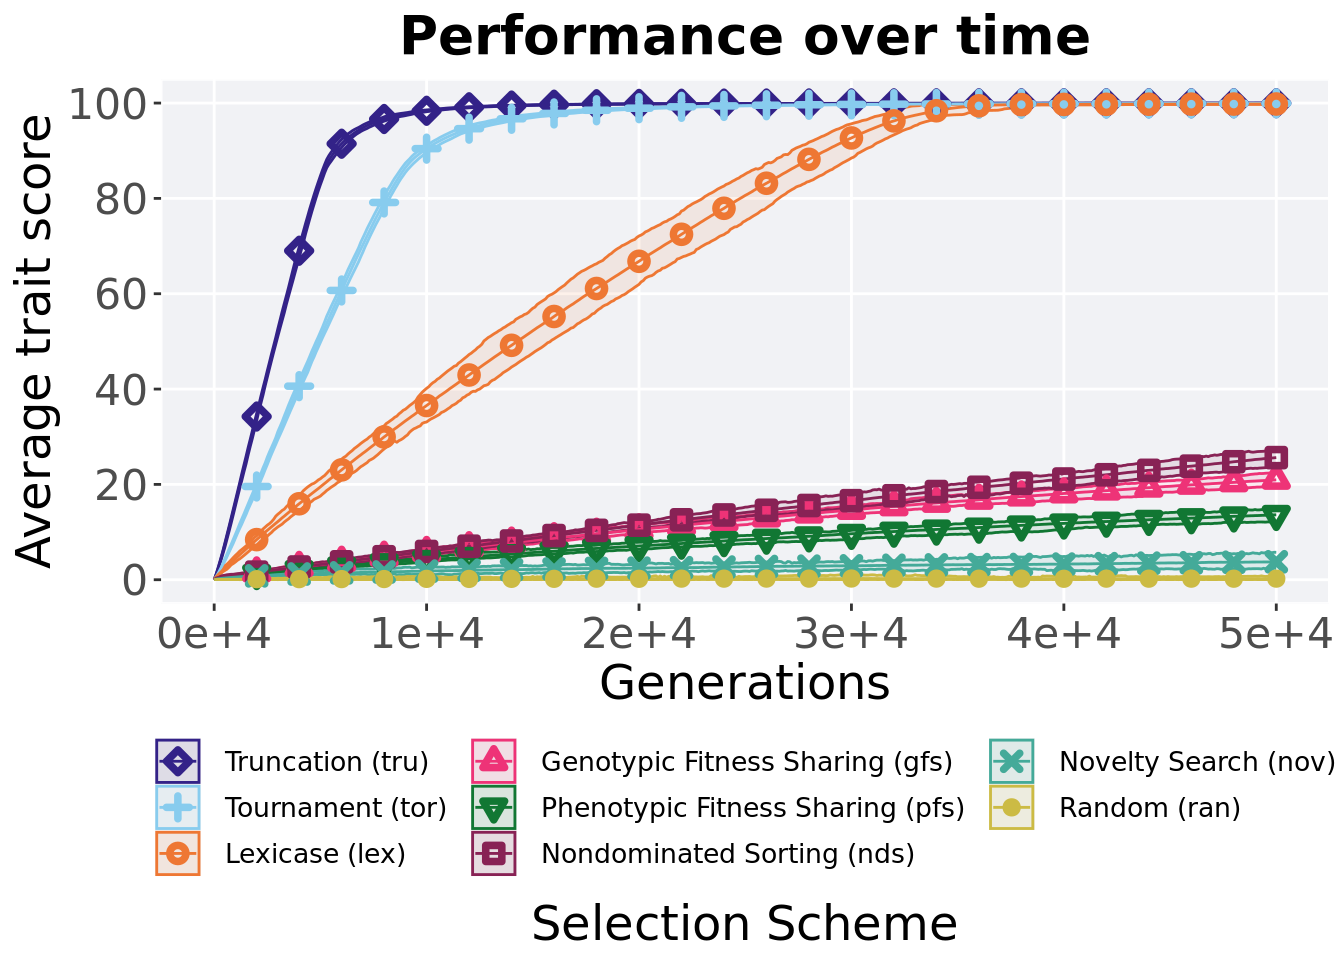
\includegraphics[width=1\linewidth]{base-diagnostics_files/figure-latex/ord-per-ot-1}

\hypertarget{best-performance-throughout-1}{%
\section{Best performance throughout}\label{best-performance-throughout-1}}

Best performance reached throughout 50,000 generations in a population.

\begin{Shaded}
\begin{Highlighting}[]
\NormalTok{plot =}\StringTok{ }\KeywordTok{filter}\NormalTok{(best_df, var }\OperatorTok{==}\StringTok{ 'pop_fit_max'}\NormalTok{) }\OperatorTok
\StringTok{  }\KeywordTok{ggplot}\NormalTok{(., }\KeywordTok{aes}\NormalTok{(}\DataTypeTok{x =}\NormalTok{ acro, }\DataTypeTok{y =}\NormalTok{ val }\OperatorTok{/}\StringTok{ }\NormalTok{DIMENSIONALITY, }\DataTypeTok{color =}\NormalTok{ acro, }\DataTypeTok{fill =}\NormalTok{ acro, }\DataTypeTok{shape =}\NormalTok{ acro)) }\OperatorTok{+}
\StringTok{  }\KeywordTok{geom_flat_violin}\NormalTok{(}\DataTypeTok{position =} \KeywordTok{position_nudge}\NormalTok{(}\DataTypeTok{x =} \FloatTok{.1}\NormalTok{, }\DataTypeTok{y =} \DecValTok{0}\NormalTok{), }\DataTypeTok{scale =} \StringTok{'width'}\NormalTok{, }\DataTypeTok{alpha =} \FloatTok{0.2}\NormalTok{, }\DataTypeTok{width =} \FloatTok{1.5}\NormalTok{) }\OperatorTok{+}
\StringTok{  }\KeywordTok{geom_boxplot}\NormalTok{(}\DataTypeTok{color =} \StringTok{'black'}\NormalTok{, }\DataTypeTok{width =} \FloatTok{.07}\NormalTok{, }\DataTypeTok{outlier.shape =} \OtherTok{NA}\NormalTok{, }\DataTypeTok{alpha =} \FloatTok{0.0}\NormalTok{, }\DataTypeTok{size =} \FloatTok{1.0}\NormalTok{, }\DataTypeTok{position =} \KeywordTok{position_nudge}\NormalTok{(}\DataTypeTok{x =} \FloatTok{.16}\NormalTok{, }\DataTypeTok{y =} \DecValTok{0}\NormalTok{)) }\OperatorTok{+}
\StringTok{  }\KeywordTok{geom_point}\NormalTok{(}\DataTypeTok{position =} \KeywordTok{position_jitter}\NormalTok{(}\DataTypeTok{width =} \FloatTok{0.03}\NormalTok{, }\DataTypeTok{height =} \FloatTok{0.02}\NormalTok{), }\DataTypeTok{size =} \FloatTok{2.0}\NormalTok{, }\DataTypeTok{alpha =} \FloatTok{1.0}\NormalTok{) }\OperatorTok{+}
\StringTok{  }\KeywordTok{scale_y_continuous}\NormalTok{(}
    \DataTypeTok{name=}\StringTok{"Average trait score"}\NormalTok{,}
    \DataTypeTok{limits=}\KeywordTok{c}\NormalTok{(}\DecValTok{0}\NormalTok{, }\DecValTok{100}\NormalTok{),}
    \DataTypeTok{breaks=}\KeywordTok{seq}\NormalTok{(}\DecValTok{0}\NormalTok{,}\DecValTok{100}\NormalTok{, }\DecValTok{20}\NormalTok{),}
    \DataTypeTok{labels=}\KeywordTok{c}\NormalTok{(}\StringTok{"0"}\NormalTok{, }\StringTok{"20"}\NormalTok{, }\StringTok{"40"}\NormalTok{, }\StringTok{"60"}\NormalTok{, }\StringTok{"80"}\NormalTok{, }\StringTok{"100"}\NormalTok{)}
\NormalTok{  ) }\OperatorTok{+}
\StringTok{  }\KeywordTok{scale_x_discrete}\NormalTok{(}
    \DataTypeTok{name=}\StringTok{"Scheme"}
\NormalTok{  )}\OperatorTok{+}
\StringTok{  }\KeywordTok{scale_shape_manual}\NormalTok{(}\DataTypeTok{values=}\NormalTok{SHAPE)}\OperatorTok{+}
\StringTok{  }\KeywordTok{scale_colour_manual}\NormalTok{(}\DataTypeTok{values =}\NormalTok{ cb_palette, ) }\OperatorTok{+}
\StringTok{  }\KeywordTok{scale_fill_manual}\NormalTok{(}\DataTypeTok{values =}\NormalTok{ cb_palette) }\OperatorTok{+}
\StringTok{  }\KeywordTok{ggtitle}\NormalTok{(}\StringTok{'Best performance throughout'}\NormalTok{)}\OperatorTok{+}
\StringTok{  }\NormalTok{p_theme}

\KeywordTok{plot_grid}\NormalTok{(}
\NormalTok{  plot }\OperatorTok{+}
\StringTok{    }\KeywordTok{theme}\NormalTok{(}\DataTypeTok{legend.position=}\StringTok{"none"}\NormalTok{),}
\NormalTok{  legend,}
  \DataTypeTok{nrow=}\DecValTok{2}\NormalTok{,}
  \DataTypeTok{rel_heights =} \KeywordTok{c}\NormalTok{(}\DecValTok{3}\NormalTok{,}\DecValTok{1}\NormalTok{)}
\NormalTok{)}
\end{Highlighting}
\end{Shaded}

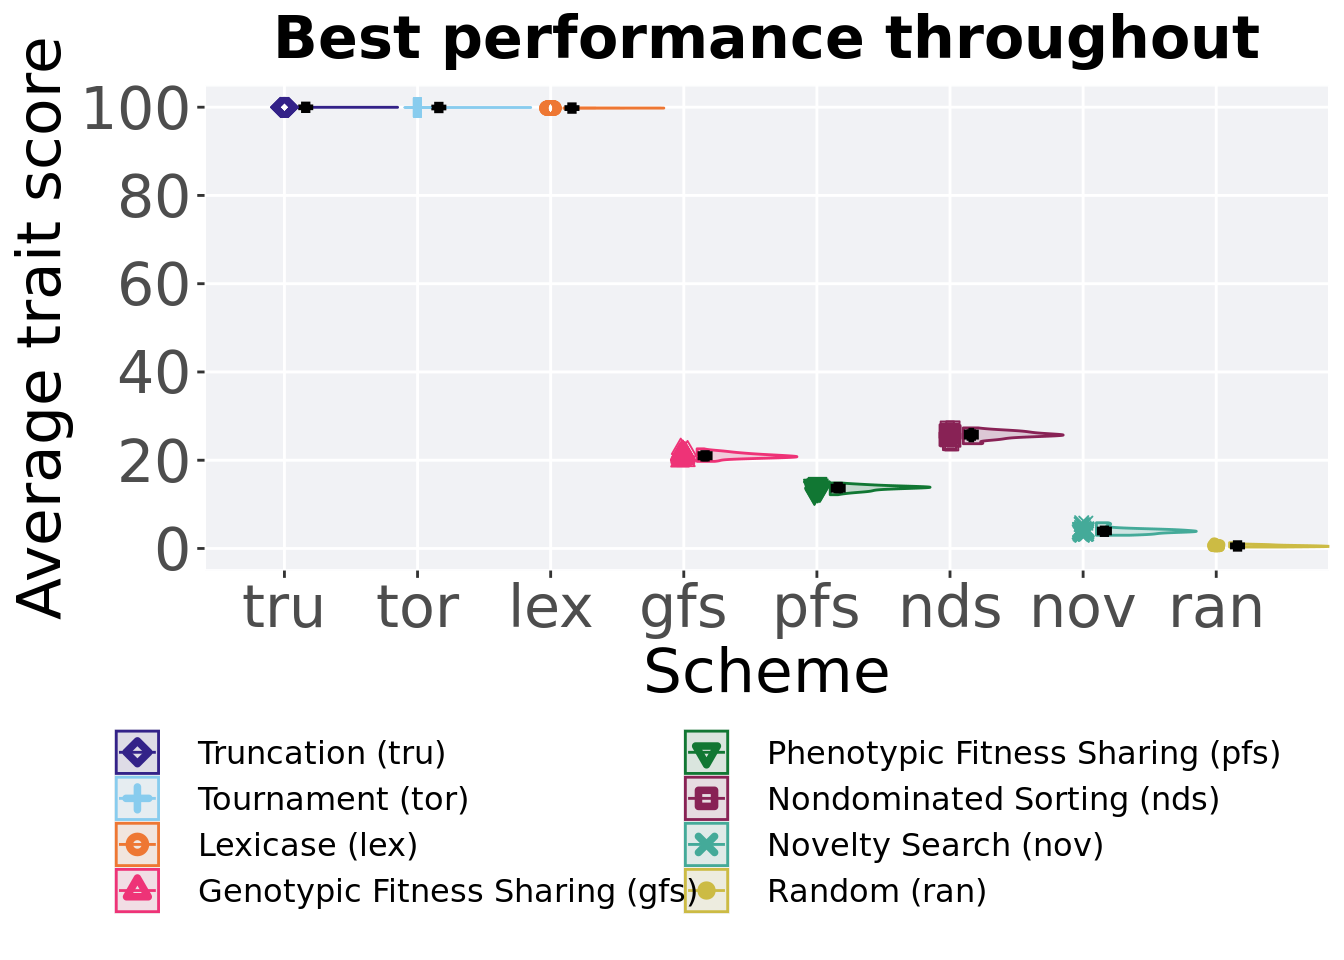
\includegraphics[width=1\linewidth]{base-diagnostics_files/figure-latex/ord-per-bst-1}

\hypertarget{stats-2}{%
\subsection{Stats}\label{stats-2}}

Summary statistics for the best performance.

\begin{Shaded}
\begin{Highlighting}[]
\NormalTok{performance =}\StringTok{ }\KeywordTok{filter}\NormalTok{(best_df, var }\OperatorTok{==}\StringTok{ 'pop_fit_max'}\NormalTok{)}
\NormalTok{performance}\OperatorTok{$}\NormalTok{acro =}\StringTok{ }\KeywordTok{factor}\NormalTok{(performance}\OperatorTok{$}\NormalTok{acro, }\DataTypeTok{levels =} \KeywordTok{c}\NormalTok{(}\StringTok{'tru'}\NormalTok{,}\StringTok{'tor'}\NormalTok{,}\StringTok{'lex'}\NormalTok{,}\StringTok{'nds'}\NormalTok{,}\StringTok{'gfs'}\NormalTok{,}\StringTok{'pfs'}\NormalTok{,}\StringTok{'nov'}\NormalTok{,}\StringTok{'ran'}\NormalTok{))}
\NormalTok{performance }\OperatorTok
\StringTok{  }\KeywordTok{group_by}\NormalTok{(acro) }\OperatorTok
\StringTok{  }\NormalTok{dplyr}\OperatorTok{::}\KeywordTok{summarise}\NormalTok{(}
    \DataTypeTok{count =} \KeywordTok{n}\NormalTok{(),}
    \DataTypeTok{na_cnt =} \KeywordTok{sum}\NormalTok{(}\KeywordTok{is.na}\NormalTok{(val)),}
    \DataTypeTok{min =} \KeywordTok{min}\NormalTok{(val }\OperatorTok{/}\StringTok{ }\NormalTok{DIMENSIONALITY, }\DataTypeTok{na.rm =} \OtherTok{TRUE}\NormalTok{),}
    \DataTypeTok{median =} \KeywordTok{median}\NormalTok{(val }\OperatorTok{/}\StringTok{ }\NormalTok{DIMENSIONALITY, }\DataTypeTok{na.rm =} \OtherTok{TRUE}\NormalTok{),}
    \DataTypeTok{mean =} \KeywordTok{mean}\NormalTok{(val }\OperatorTok{/}\StringTok{ }\NormalTok{DIMENSIONALITY, }\DataTypeTok{na.rm =} \OtherTok{TRUE}\NormalTok{),}
    \DataTypeTok{max =} \KeywordTok{max}\NormalTok{(val }\OperatorTok{/}\StringTok{ }\NormalTok{DIMENSIONALITY, }\DataTypeTok{na.rm =} \OtherTok{TRUE}\NormalTok{),}
    \DataTypeTok{IQR =} \KeywordTok{IQR}\NormalTok{(val }\OperatorTok{/}\StringTok{ }\NormalTok{DIMENSIONALITY, }\DataTypeTok{na.rm =} \OtherTok{TRUE}\NormalTok{)}
\NormalTok{  )}
\end{Highlighting}
\end{Shaded}

\begin{verbatim}
## # A tibble: 8 x 8
##   acro  count na_cnt     min  median    mean    max     IQR
##   <fct> <int>  <int>   <dbl>   <dbl>   <dbl>  <dbl>   <dbl>
## 1 tru      50      0 100.    100.    100.    100.   0.00168
## 2 tor      50      0  99.9    99.9    99.9    99.9  0.00650
## 3 lex      50      0  99.7    99.8    99.8    99.9  0.0247 
## 4 nds      50      0  23.7    25.7    25.7    27.3  0.972  
## 5 gfs      50      0  19.7    21.0    21.0    22.6  0.754  
## 6 pfs      50      0  12.2    13.8    13.7    14.9  0.712  
## 7 nov      50      0   3.00    3.90    4.00    5.83 0.666  
## 8 ran      50      0   0.318   0.569   0.605   1.31 0.279
\end{verbatim}

Kruskal--Wallis test illustrates evidence of statistical differences.

\begin{Shaded}
\begin{Highlighting}[]
\KeywordTok{kruskal.test}\NormalTok{(val }\OperatorTok{~}\StringTok{ }\NormalTok{acro, }\DataTypeTok{data =}\NormalTok{ performance)}
\end{Highlighting}
\end{Shaded}

\begin{verbatim}
## 
##  Kruskal-Wallis rank sum test
## 
## data:  val by acro
## Kruskal-Wallis chi-squared = 392.77, df = 7, p-value < 2.2e-16
\end{verbatim}

Results for post-hoc Wilcoxon rank-sum test with a Bonferroni correction.

\begin{Shaded}
\begin{Highlighting}[]
\KeywordTok{pairwise.wilcox.test}\NormalTok{(}\DataTypeTok{x =}\NormalTok{ performance}\OperatorTok{$}\NormalTok{val, }\DataTypeTok{g =}\NormalTok{ performance}\OperatorTok{$}\NormalTok{acro, }\DataTypeTok{p.adjust.method =} \StringTok{"bonferroni"}\NormalTok{,}
                     \DataTypeTok{paired =} \OtherTok{FALSE}\NormalTok{, }\DataTypeTok{conf.int =} \OtherTok{FALSE}\NormalTok{, }\DataTypeTok{alternative =} \StringTok{'l'}\NormalTok{)}
\end{Highlighting}
\end{Shaded}

\begin{verbatim}
## 
##  Pairwise comparisons using Wilcoxon rank sum test with continuity correction 
## 
## data:  performance$val and performance$acro 
## 
##     tru    tor    lex    nds    gfs    pfs    nov   
## tor <2e-16 -      -      -      -      -      -     
## lex <2e-16 <2e-16 -      -      -      -      -     
## nds <2e-16 <2e-16 <2e-16 -      -      -      -     
## gfs <2e-16 <2e-16 <2e-16 <2e-16 -      -      -     
## pfs <2e-16 <2e-16 <2e-16 <2e-16 <2e-16 -      -     
## nov <2e-16 <2e-16 <2e-16 <2e-16 <2e-16 <2e-16 -     
## ran <2e-16 <2e-16 <2e-16 <2e-16 <2e-16 <2e-16 <2e-16
## 
## P value adjustment method: bonferroni
\end{verbatim}

\hypertarget{generation-satisfactory-solution-found-1}{%
\section{Generation satisfactory solution found}\label{generation-satisfactory-solution-found-1}}

First generation a satisfactory solution is found throughout the 50,000 generations.

\begin{Shaded}
\begin{Highlighting}[]
\NormalTok{plot =}\StringTok{ }\NormalTok{sati_df }\OperatorTok
\StringTok{  }\KeywordTok{ggplot}\NormalTok{(., }\KeywordTok{aes}\NormalTok{(}\DataTypeTok{x =}\NormalTok{ acro, }\DataTypeTok{y =}\NormalTok{ gen , }\DataTypeTok{color =}\NormalTok{ acro, }\DataTypeTok{fill =}\NormalTok{ acro, }\DataTypeTok{shape =}\NormalTok{ acro)) }\OperatorTok{+}
\StringTok{  }\KeywordTok{geom_flat_violin}\NormalTok{(}\DataTypeTok{position =} \KeywordTok{position_nudge}\NormalTok{(}\DataTypeTok{x =} \FloatTok{.1}\NormalTok{, }\DataTypeTok{y =} \DecValTok{0}\NormalTok{), }\DataTypeTok{scale =} \StringTok{'width'}\NormalTok{, }\DataTypeTok{alpha =} \FloatTok{0.2}\NormalTok{, }\DataTypeTok{width =} \FloatTok{1.5}\NormalTok{) }\OperatorTok{+}
\StringTok{  }\KeywordTok{geom_boxplot}\NormalTok{(}\DataTypeTok{color =} \StringTok{'black'}\NormalTok{, }\DataTypeTok{width =} \FloatTok{.07}\NormalTok{, }\DataTypeTok{outlier.shape =} \OtherTok{NA}\NormalTok{, }\DataTypeTok{alpha =} \FloatTok{0.0}\NormalTok{, }\DataTypeTok{size =} \FloatTok{1.0}\NormalTok{, }\DataTypeTok{position =} \KeywordTok{position_nudge}\NormalTok{(}\DataTypeTok{x =} \FloatTok{.16}\NormalTok{, }\DataTypeTok{y =} \DecValTok{0}\NormalTok{)) }\OperatorTok{+}
\StringTok{  }\KeywordTok{geom_point}\NormalTok{(}\DataTypeTok{position =} \KeywordTok{position_jitter}\NormalTok{(}\DataTypeTok{width =} \FloatTok{0.03}\NormalTok{, }\DataTypeTok{height =} \FloatTok{0.02}\NormalTok{), }\DataTypeTok{size =} \FloatTok{2.0}\NormalTok{, }\DataTypeTok{alpha =} \FloatTok{1.0}\NormalTok{) }\OperatorTok{+}
\StringTok{  }\KeywordTok{scale_y_continuous}\NormalTok{(}
    \DataTypeTok{name=}\StringTok{"Generation"}\NormalTok{,}
    \DataTypeTok{limits=}\KeywordTok{c}\NormalTok{(}\DecValTok{0}\NormalTok{, }\DecValTok{60001}\NormalTok{),}
    \DataTypeTok{breaks=}\KeywordTok{c}\NormalTok{(}\DecValTok{0}\NormalTok{, }\DecValTok{10000}\NormalTok{, }\DecValTok{20000}\NormalTok{, }\DecValTok{30000}\NormalTok{, }\DecValTok{40000}\NormalTok{, }\DecValTok{50000}\NormalTok{, }\DecValTok{60000}\NormalTok{),}
    \DataTypeTok{labels=}\KeywordTok{c}\NormalTok{(}\StringTok{"0e+4"}\NormalTok{, }\StringTok{"1e+4"}\NormalTok{, }\StringTok{"2e+4"}\NormalTok{, }\StringTok{"3e+4"}\NormalTok{, }\StringTok{"4e+4"}\NormalTok{, }\StringTok{"5e+4"}\NormalTok{, }\StringTok{"Fail"}\NormalTok{)}
\NormalTok{  ) }\OperatorTok{+}
\StringTok{  }\KeywordTok{scale_x_discrete}\NormalTok{(}
    \DataTypeTok{name=}\StringTok{"Scheme"}
\NormalTok{  )}\OperatorTok{+}
\StringTok{  }\KeywordTok{scale_shape_manual}\NormalTok{(}\DataTypeTok{values=}\NormalTok{SHAPE)}\OperatorTok{+}
\StringTok{  }\KeywordTok{scale_colour_manual}\NormalTok{(}\DataTypeTok{values =}\NormalTok{ cb_palette, ) }\OperatorTok{+}
\StringTok{  }\KeywordTok{scale_fill_manual}\NormalTok{(}\DataTypeTok{values =}\NormalTok{ cb_palette) }\OperatorTok{+}
\StringTok{  }\KeywordTok{ggtitle}\NormalTok{(}\StringTok{'Generation satisfactory solution found'}\NormalTok{)}\OperatorTok{+}
\StringTok{  }\NormalTok{p_theme}

\KeywordTok{plot_grid}\NormalTok{(}
\NormalTok{  plot }\OperatorTok{+}
\StringTok{    }\KeywordTok{theme}\NormalTok{(}\DataTypeTok{legend.position=}\StringTok{"none"}\NormalTok{),}
\NormalTok{  legend,}
  \DataTypeTok{nrow=}\DecValTok{2}\NormalTok{,}
  \DataTypeTok{rel_heights =} \KeywordTok{c}\NormalTok{(}\DecValTok{3}\NormalTok{,}\DecValTok{1}\NormalTok{)}
\NormalTok{)}
\end{Highlighting}
\end{Shaded}

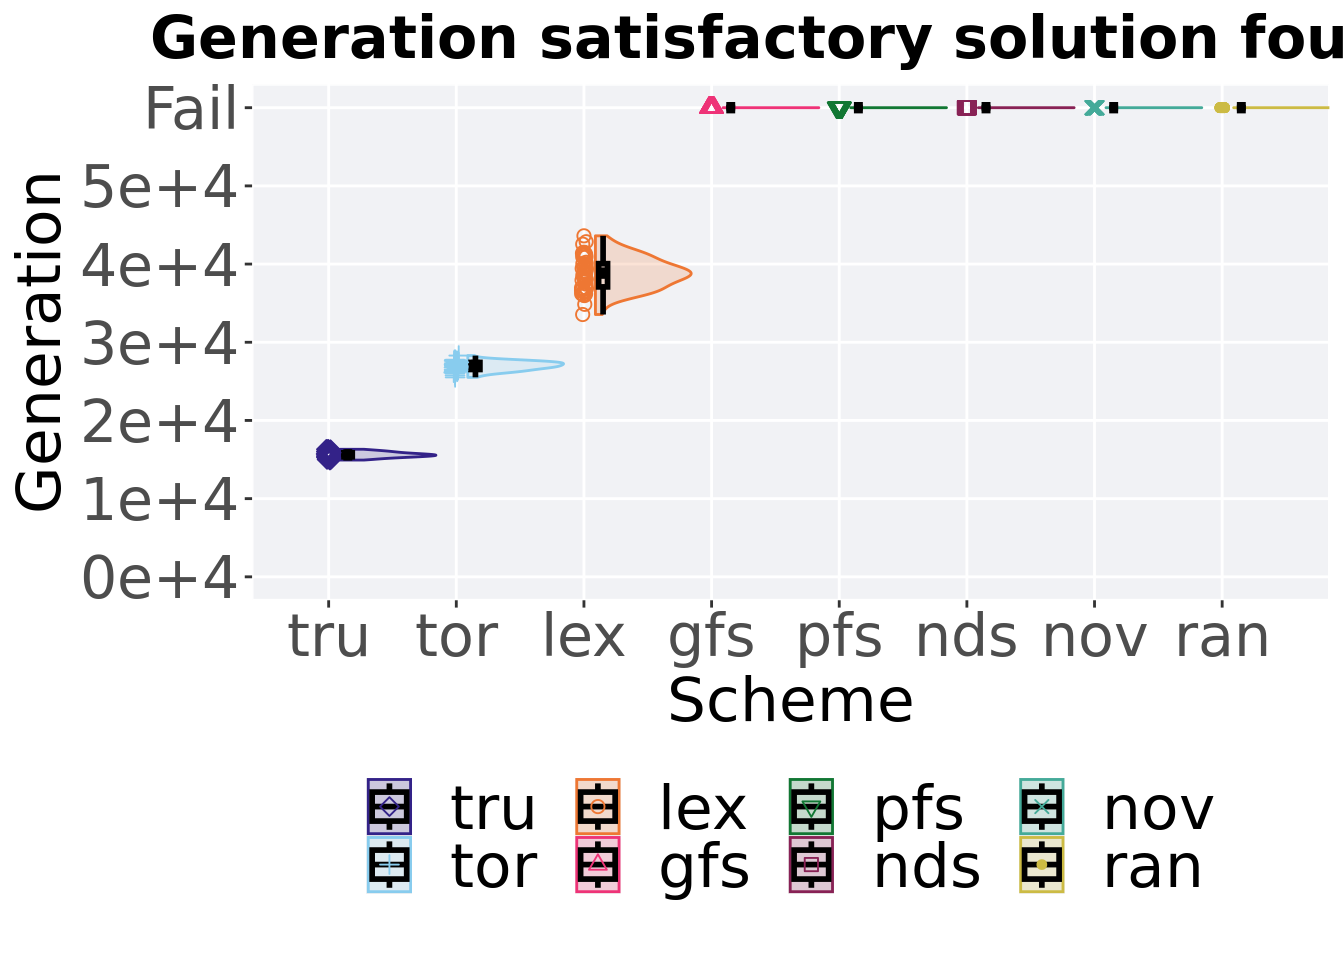
\includegraphics[width=1\linewidth]{base-diagnostics_files/figure-latex/ord-ssf-1}

\hypertarget{stats-3}{%
\subsection{Stats}\label{stats-3}}

Summary statistics for the generation a satisfactory solution is found.

\begin{Shaded}
\begin{Highlighting}[]
\NormalTok{ssf =}\StringTok{ }\KeywordTok{filter}\NormalTok{(sati_df, gen }\OperatorTok{<=}\StringTok{ }\NormalTok{GENERATIONS)}
\NormalTok{ssf}\OperatorTok{$}\NormalTok{acro =}\StringTok{ }\KeywordTok{factor}\NormalTok{(ssf}\OperatorTok{$}\NormalTok{acro, }\DataTypeTok{levels =} \KeywordTok{c}\NormalTok{(}\StringTok{'tru'}\NormalTok{,}\StringTok{'tor'}\NormalTok{,}\StringTok{'lex'}\NormalTok{))}
\NormalTok{ssf }\OperatorTok
\StringTok{  }\KeywordTok{group_by}\NormalTok{(acro) }\OperatorTok
\StringTok{  }\NormalTok{dplyr}\OperatorTok{::}\KeywordTok{summarise}\NormalTok{(}
    \DataTypeTok{count =} \KeywordTok{n}\NormalTok{(),}
    \DataTypeTok{na_cnt =} \KeywordTok{sum}\NormalTok{(}\KeywordTok{is.na}\NormalTok{(gen)),}
    \DataTypeTok{min =} \KeywordTok{min}\NormalTok{(gen, }\DataTypeTok{na.rm =} \OtherTok{TRUE}\NormalTok{),}
    \DataTypeTok{median =} \KeywordTok{median}\NormalTok{(gen, }\DataTypeTok{na.rm =} \OtherTok{TRUE}\NormalTok{),}
    \DataTypeTok{mean =} \KeywordTok{mean}\NormalTok{(gen, }\DataTypeTok{na.rm =} \OtherTok{TRUE}\NormalTok{),}
    \DataTypeTok{max =} \KeywordTok{max}\NormalTok{(gen, }\DataTypeTok{na.rm =} \OtherTok{TRUE}\NormalTok{),}
    \DataTypeTok{IQR =} \KeywordTok{IQR}\NormalTok{(gen, }\DataTypeTok{na.rm =} \OtherTok{TRUE}\NormalTok{)}
\NormalTok{  )}
\end{Highlighting}
\end{Shaded}

\begin{verbatim}
## # A tibble: 3 x 8
##   acro  count na_cnt   min median   mean   max   IQR
##   <fct> <int>  <int> <int>  <dbl>  <dbl> <int> <dbl>
## 1 tru      50      0 14776 15585  15570. 16317  420.
## 2 tor      50      0 25996 27138  27105. 28495  913.
## 3 lex      50      0 33877 38288. 38265. 43565 2215.
\end{verbatim}

Kruskal--Wallis test illustrates evidence of statistical differences.

\begin{Shaded}
\begin{Highlighting}[]
\KeywordTok{kruskal.test}\NormalTok{(gen }\OperatorTok{~}\StringTok{ }\NormalTok{acro, }\DataTypeTok{data =}\NormalTok{ ssf)}
\end{Highlighting}
\end{Shaded}

\begin{verbatim}
## 
##  Kruskal-Wallis rank sum test
## 
## data:  gen by acro
## Kruskal-Wallis chi-squared = 132.45, df = 2, p-value < 2.2e-16
\end{verbatim}

Results for post-hoc Wilcoxon rank-sum test with a Bonferroni correction.

\begin{Shaded}
\begin{Highlighting}[]
\KeywordTok{pairwise.wilcox.test}\NormalTok{(}\DataTypeTok{x =}\NormalTok{ ssf}\OperatorTok{$}\NormalTok{gen, }\DataTypeTok{g =}\NormalTok{ ssf}\OperatorTok{$}\NormalTok{acro, }\DataTypeTok{p.adjust.method =} \StringTok{"bonferroni"}\NormalTok{,}
                     \DataTypeTok{paired =} \OtherTok{FALSE}\NormalTok{, }\DataTypeTok{conf.int =} \OtherTok{FALSE}\NormalTok{, }\DataTypeTok{alternative =} \StringTok{'g'}\NormalTok{)}
\end{Highlighting}
\end{Shaded}

\begin{verbatim}
## 
##  Pairwise comparisons using Wilcoxon rank sum test with continuity correction 
## 
## data:  ssf$gen and ssf$acro 
## 
##     tru    tor   
## tor <2e-16 -     
## lex <2e-16 <2e-16
## 
## P value adjustment method: bonferroni
\end{verbatim}

\hypertarget{streaks-over-time}{%
\section{Streaks over time}\label{streaks-over-time}}

Longest streak of active geens for the best solution found in a population over time.
A maximum streak value of 100 and a minimum streak value of 1 is possible.
Data points on the graph is the average streak across 50 replicates every 2000 generations.
Shading comes from the best and worse streak across 50 replicates.

\begin{Shaded}
\begin{Highlighting}[]
\NormalTok{lines =}\StringTok{ }\KeywordTok{filter}\NormalTok{(over_time_df, acro }\OperatorTok{!=}\StringTok{ 'tor'} \OperatorTok{&}\StringTok{ }\NormalTok{acro }\OperatorTok{!=}\StringTok{ 'tru'} \OperatorTok{&}\StringTok{ }\NormalTok{acro }\OperatorTok{!=}\StringTok{ 'lex'}\NormalTok{) }\OperatorTok
\StringTok{  }\KeywordTok{group_by}\NormalTok{(scheme, gen) }\OperatorTok
\StringTok{  }\NormalTok{dplyr}\OperatorTok{::}\KeywordTok{summarise}\NormalTok{(}
    \DataTypeTok{min =} \KeywordTok{min}\NormalTok{(ele_stk_cnt),}
    \DataTypeTok{mean =} \KeywordTok{mean}\NormalTok{(ele_stk_cnt),}
    \DataTypeTok{max =} \KeywordTok{max}\NormalTok{(ele_stk_cnt)}
\NormalTok{  )}
\end{Highlighting}
\end{Shaded}

\begin{verbatim}
## `summarise()` has grouped output by 'scheme'. You can override using the
## `.groups` argument.
\end{verbatim}

\begin{Shaded}
\begin{Highlighting}[]
\NormalTok{over_time_plot =}\StringTok{ }\KeywordTok{ggplot}\NormalTok{(lines, }\KeywordTok{aes}\NormalTok{(}\DataTypeTok{x=}\NormalTok{gen, }\DataTypeTok{y=}\NormalTok{mean, }\DataTypeTok{group =}\NormalTok{ scheme, }\DataTypeTok{fill =}\NormalTok{ scheme, }\DataTypeTok{color =}\NormalTok{ scheme, }\DataTypeTok{shape =}\NormalTok{ scheme)) }\OperatorTok{+}
\StringTok{  }\KeywordTok{geom_ribbon}\NormalTok{(}\KeywordTok{aes}\NormalTok{(}\DataTypeTok{ymin =}\NormalTok{ min, }\DataTypeTok{ymax =}\NormalTok{ max), }\DataTypeTok{alpha =} \FloatTok{0.1}\NormalTok{) }\OperatorTok{+}
\StringTok{  }\KeywordTok{geom_line}\NormalTok{(}\DataTypeTok{size =} \FloatTok{0.5}\NormalTok{) }\OperatorTok{+}
\StringTok{  }\KeywordTok{geom_point}\NormalTok{(}\DataTypeTok{data =} \KeywordTok{filter}\NormalTok{(lines, gen }\OperatorTok\StringTok{ }\DecValTok{2000} \OperatorTok{==}\StringTok{ }\DecValTok{0} \OperatorTok{&}\StringTok{ }\NormalTok{gen }\OperatorTok{!=}\StringTok{ }\DecValTok{0}\NormalTok{), }\DataTypeTok{size =} \FloatTok{1.5}\NormalTok{, }\DataTypeTok{stroke =} \FloatTok{2.0}\NormalTok{, }\DataTypeTok{alpha =} \FloatTok{1.0}\NormalTok{) }\OperatorTok{+}
\StringTok{  }\KeywordTok{scale_y_continuous}\NormalTok{(}
    \DataTypeTok{name=}\StringTok{"Streak"}\NormalTok{,}
    \DataTypeTok{limits=}\KeywordTok{c}\NormalTok{(}\DecValTok{0}\NormalTok{, }\DecValTok{45}\NormalTok{),}
    \DataTypeTok{breaks=}\KeywordTok{seq}\NormalTok{(}\DecValTok{0}\NormalTok{,}\DecValTok{45}\NormalTok{, }\DecValTok{15}\NormalTok{)}
\NormalTok{  ) }\OperatorTok{+}
\StringTok{  }\KeywordTok{scale_x_continuous}\NormalTok{(}
    \DataTypeTok{name=}\StringTok{"Generations"}\NormalTok{,}
    \DataTypeTok{limits=}\KeywordTok{c}\NormalTok{(}\DecValTok{0}\NormalTok{, }\DecValTok{50000}\NormalTok{),}
    \DataTypeTok{breaks=}\KeywordTok{c}\NormalTok{(}\DecValTok{0}\NormalTok{, }\DecValTok{10000}\NormalTok{, }\DecValTok{20000}\NormalTok{, }\DecValTok{30000}\NormalTok{, }\DecValTok{40000}\NormalTok{, }\DecValTok{50000}\NormalTok{),}
    \DataTypeTok{labels=}\KeywordTok{c}\NormalTok{(}\StringTok{"0e+4"}\NormalTok{, }\StringTok{"1e+4"}\NormalTok{, }\StringTok{"2e+4"}\NormalTok{, }\StringTok{"3e+4"}\NormalTok{, }\StringTok{"4e+4"}\NormalTok{, }\StringTok{"5e+4"}\NormalTok{)}

\NormalTok{  ) }\OperatorTok{+}
\StringTok{  }\KeywordTok{scale_shape_manual}\NormalTok{(}\DataTypeTok{values=}\NormalTok{STK_SHAPE)}\OperatorTok{+}
\StringTok{  }\KeywordTok{scale_colour_manual}\NormalTok{(}\DataTypeTok{values =}\NormalTok{ stk_cb_palette) }\OperatorTok{+}
\StringTok{  }\KeywordTok{scale_fill_manual}\NormalTok{(}\DataTypeTok{values =}\NormalTok{ stk_cb_palette) }\OperatorTok{+}
\StringTok{  }\KeywordTok{ggtitle}\NormalTok{(}\StringTok{'Longest streak over time'}\NormalTok{)}\OperatorTok{+}
\StringTok{  }\NormalTok{p_theme }\OperatorTok{+}
\StringTok{  }\KeywordTok{guides}\NormalTok{(}
    \DataTypeTok{shape=}\KeywordTok{guide_legend}\NormalTok{(}\DataTypeTok{ncol=}\DecValTok{2}\NormalTok{, }\DataTypeTok{title.position =} \StringTok{"left"}\NormalTok{, }\DataTypeTok{title =} \StringTok{'Selection }\CharTok{\textbackslash{}n}\StringTok{Scheme'}\NormalTok{),}
    \DataTypeTok{color=}\KeywordTok{guide_legend}\NormalTok{(}\DataTypeTok{ncol=}\DecValTok{2}\NormalTok{, }\DataTypeTok{title.position =} \StringTok{"left"}\NormalTok{, }\DataTypeTok{title =} \StringTok{'Selection }\CharTok{\textbackslash{}n}\StringTok{Scheme'}\NormalTok{),}
    \DataTypeTok{fill=}\KeywordTok{guide_legend}\NormalTok{(}\DataTypeTok{ncol=}\DecValTok{2}\NormalTok{, }\DataTypeTok{title.position =} \StringTok{"left"}\NormalTok{, }\DataTypeTok{title =} \StringTok{'Selection }\CharTok{\textbackslash{}n}\StringTok{Scheme'}\NormalTok{)}
\NormalTok{  )}

\NormalTok{over_time_plot}
\end{Highlighting}
\end{Shaded}

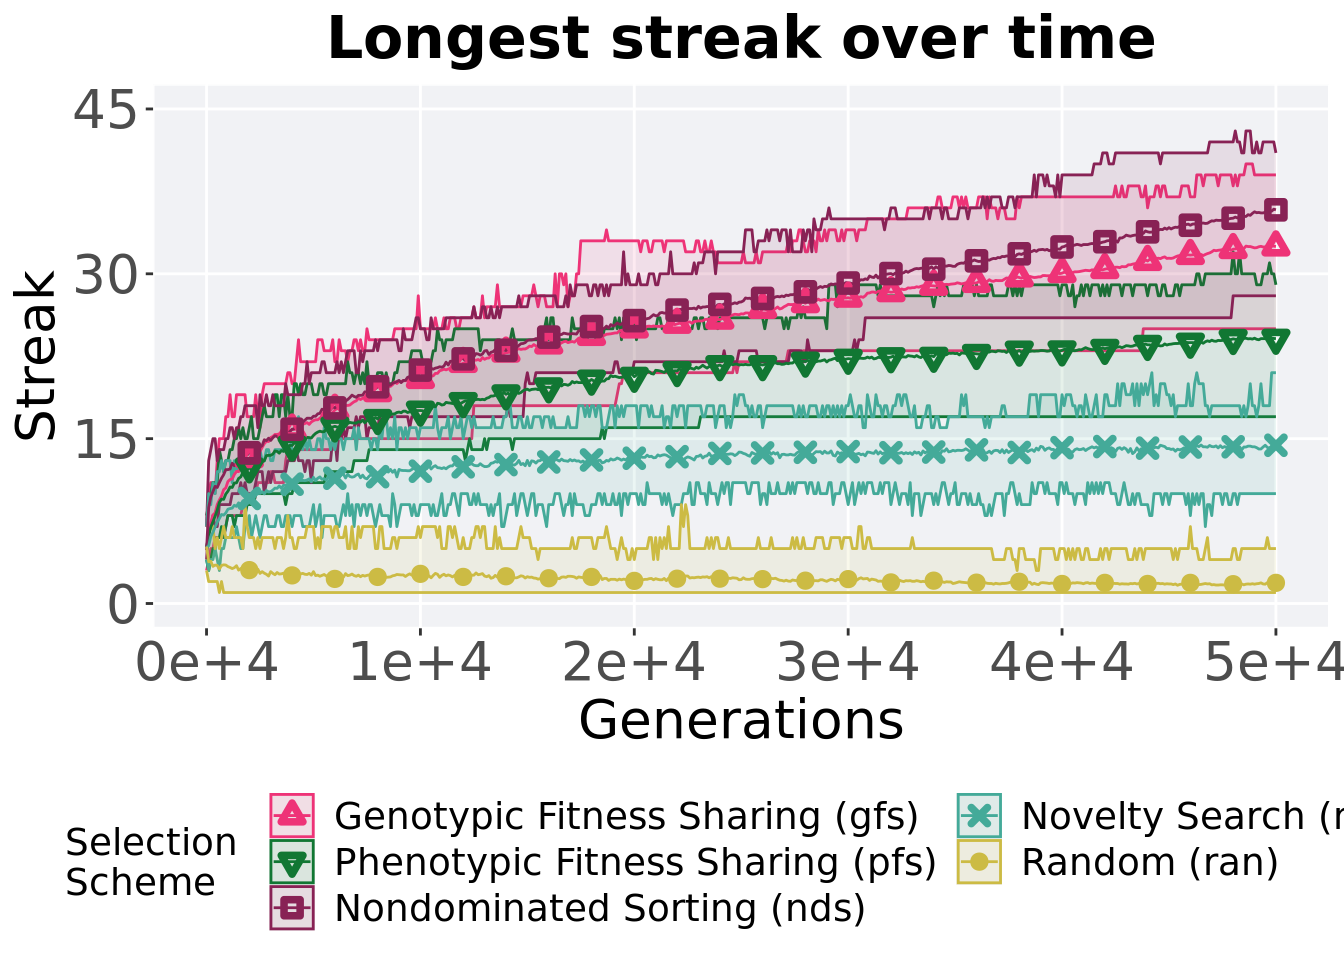
\includegraphics[width=1\linewidth]{base-diagnostics_files/figure-latex/ord-str-ot-1}

\hypertarget{longest-streak-throughout}{%
\section{Longest streak throughout}\label{longest-streak-throughout}}

Longest streak of the best solution found in the population throughout 50,000 generations.

\begin{Shaded}
\begin{Highlighting}[]
\NormalTok{plot =}\StringTok{ }\KeywordTok{filter}\NormalTok{(best_df, var }\OperatorTok{==}\StringTok{ 'ele_stk_cnt'} \OperatorTok{&}\StringTok{  }\NormalTok{acro }\OperatorTok{!=}\StringTok{ 'tor'} \OperatorTok{&}\StringTok{ }\NormalTok{acro }\OperatorTok{!=}\StringTok{ 'tru'} \OperatorTok{&}\StringTok{ }\NormalTok{acro }\OperatorTok{!=}\StringTok{ 'lex'}\NormalTok{) }\OperatorTok
\StringTok{  }\KeywordTok{ggplot}\NormalTok{(., }\KeywordTok{aes}\NormalTok{(}\DataTypeTok{x =}\NormalTok{ acro, }\DataTypeTok{y =}\NormalTok{ val, }\DataTypeTok{color =}\NormalTok{ acro, }\DataTypeTok{fill =}\NormalTok{ acro, }\DataTypeTok{shape =}\NormalTok{ acro)) }\OperatorTok{+}
\StringTok{  }\KeywordTok{geom_flat_violin}\NormalTok{(}\DataTypeTok{position =} \KeywordTok{position_nudge}\NormalTok{(}\DataTypeTok{x =} \FloatTok{.1}\NormalTok{, }\DataTypeTok{y =} \DecValTok{0}\NormalTok{), }\DataTypeTok{scale =} \StringTok{'width'}\NormalTok{, }\DataTypeTok{alpha =} \FloatTok{0.2}\NormalTok{, }\DataTypeTok{width =} \FloatTok{1.5}\NormalTok{) }\OperatorTok{+}
\StringTok{  }\KeywordTok{geom_boxplot}\NormalTok{(}\DataTypeTok{color =} \StringTok{'black'}\NormalTok{, }\DataTypeTok{width =} \FloatTok{.07}\NormalTok{, }\DataTypeTok{outlier.shape =} \OtherTok{NA}\NormalTok{, }\DataTypeTok{alpha =} \FloatTok{0.0}\NormalTok{, }\DataTypeTok{size =} \FloatTok{1.0}\NormalTok{, }\DataTypeTok{position =} \KeywordTok{position_nudge}\NormalTok{(}\DataTypeTok{x =} \FloatTok{.16}\NormalTok{, }\DataTypeTok{y =} \DecValTok{0}\NormalTok{)) }\OperatorTok{+}
\StringTok{  }\KeywordTok{geom_point}\NormalTok{(}\DataTypeTok{position =} \KeywordTok{position_jitter}\NormalTok{(}\DataTypeTok{width =} \FloatTok{0.03}\NormalTok{, }\DataTypeTok{height =} \FloatTok{0.02}\NormalTok{), }\DataTypeTok{size =} \FloatTok{2.0}\NormalTok{, }\DataTypeTok{alpha =} \FloatTok{1.0}\NormalTok{) }\OperatorTok{+}
\StringTok{  }\KeywordTok{scale_y_continuous}\NormalTok{(}
    \DataTypeTok{name=}\StringTok{"Streak"}\NormalTok{,}
    \DataTypeTok{limits=}\KeywordTok{c}\NormalTok{(}\DecValTok{0}\NormalTok{, }\DecValTok{45}\NormalTok{),}
    \DataTypeTok{breaks=}\KeywordTok{seq}\NormalTok{(}\DecValTok{0}\NormalTok{,}\DecValTok{45}\NormalTok{, }\DecValTok{15}\NormalTok{)}
\NormalTok{  ) }\OperatorTok{+}
\StringTok{  }\KeywordTok{scale_x_discrete}\NormalTok{(}
    \DataTypeTok{name=}\StringTok{"Scheme"}
\NormalTok{  )}\OperatorTok{+}
\StringTok{  }\KeywordTok{scale_shape_manual}\NormalTok{(}\DataTypeTok{values=}\NormalTok{STK_SHAPE)}\OperatorTok{+}
\StringTok{  }\KeywordTok{scale_colour_manual}\NormalTok{(}\DataTypeTok{values =}\NormalTok{ stk_cb_palette) }\OperatorTok{+}
\StringTok{  }\KeywordTok{scale_fill_manual}\NormalTok{(}\DataTypeTok{values =}\NormalTok{ stk_cb_palette) }\OperatorTok{+}
\StringTok{  }\KeywordTok{ggtitle}\NormalTok{(}\StringTok{'Longest streak throughout'}\NormalTok{)}\OperatorTok{+}
\StringTok{  }\NormalTok{p_theme }\OperatorTok{+}\StringTok{ }\KeywordTok{theme}\NormalTok{(}\DataTypeTok{legend.title=}\KeywordTok{element_blank}\NormalTok{())}

\KeywordTok{plot_grid}\NormalTok{(}
\NormalTok{  plot }\OperatorTok{+}
\StringTok{    }\KeywordTok{theme}\NormalTok{(}\DataTypeTok{legend.position=}\StringTok{"none"}\NormalTok{),}
\NormalTok{  legend,}
  \DataTypeTok{nrow=}\DecValTok{2}\NormalTok{,}
  \DataTypeTok{rel_heights =} \KeywordTok{c}\NormalTok{(}\DecValTok{3}\NormalTok{,}\DecValTok{1}\NormalTok{)}
\NormalTok{)}
\end{Highlighting}
\end{Shaded}

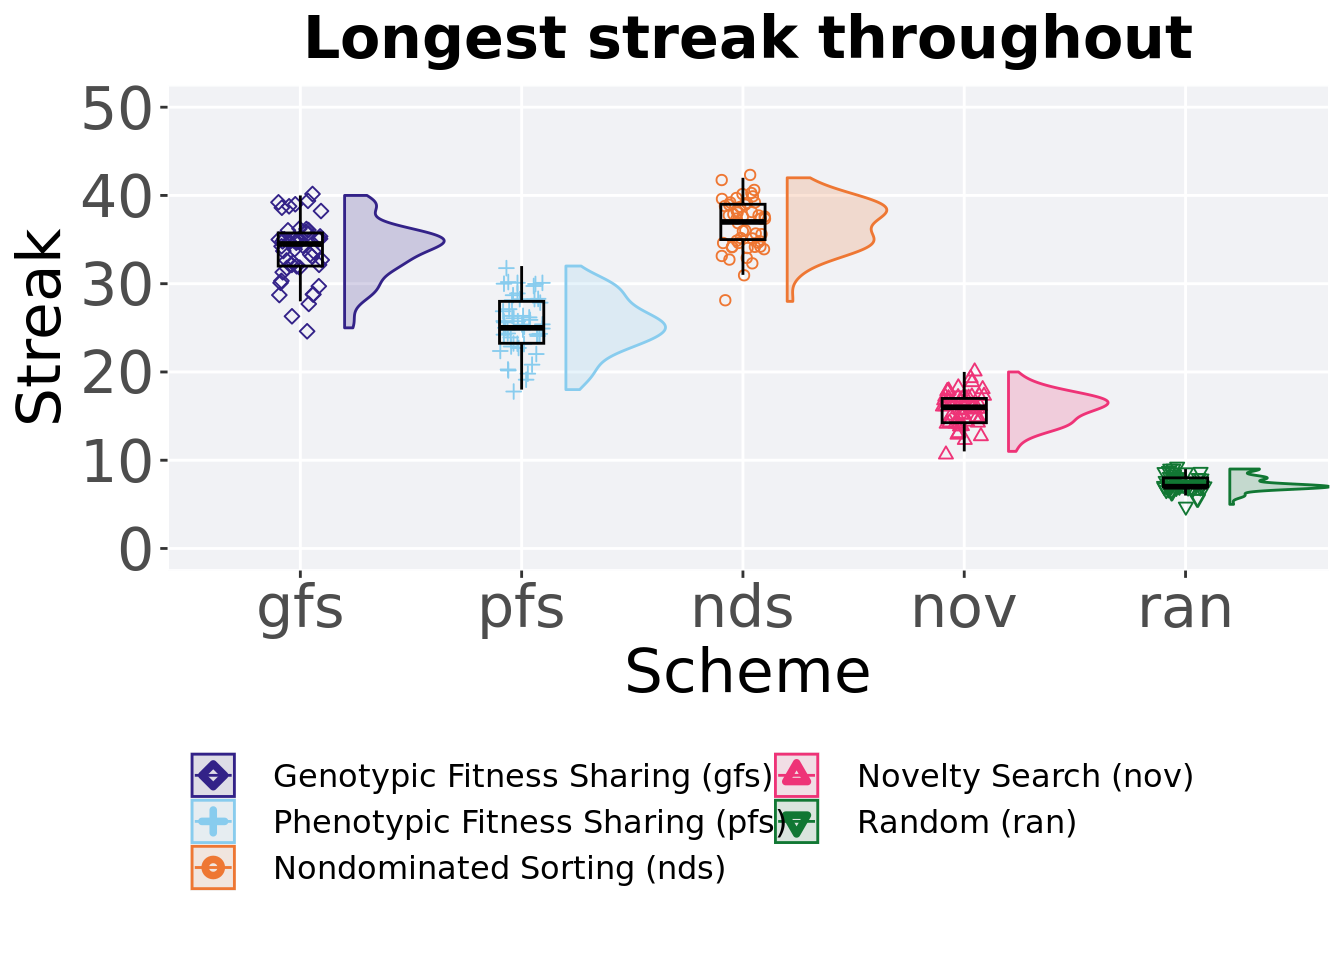
\includegraphics[width=1\linewidth]{base-diagnostics_files/figure-latex/ord-str-bst-1}

\hypertarget{stats-4}{%
\subsection{Stats}\label{stats-4}}

Summary statistics for the longest streak

\begin{Shaded}
\begin{Highlighting}[]
\NormalTok{streak =}\StringTok{ }\KeywordTok{filter}\NormalTok{(best_df, var }\OperatorTok{==}\StringTok{ 'ele_stk_cnt'} \OperatorTok{&}\StringTok{  }\NormalTok{acro }\OperatorTok{!=}\StringTok{ 'tor'} \OperatorTok{&}\StringTok{ }\NormalTok{acro }\OperatorTok{!=}\StringTok{ 'tru'} \OperatorTok{&}\StringTok{ }\NormalTok{acro }\OperatorTok{!=}\StringTok{ 'lex'}\NormalTok{)}
\NormalTok{streak}\OperatorTok{$}\NormalTok{acro =}\StringTok{ }\KeywordTok{factor}\NormalTok{(streak}\OperatorTok{$}\NormalTok{acro, }\DataTypeTok{levels =} \KeywordTok{c}\NormalTok{(}\StringTok{'nds'}\NormalTok{,}\StringTok{'gfs'}\NormalTok{,}\StringTok{'pfs'}\NormalTok{,}\StringTok{'nov'}\NormalTok{,}\StringTok{'ran'}\NormalTok{))}
\NormalTok{streak }\OperatorTok
\StringTok{  }\KeywordTok{group_by}\NormalTok{(acro) }\OperatorTok
\StringTok{  }\NormalTok{dplyr}\OperatorTok{::}\KeywordTok{summarise}\NormalTok{(}
    \DataTypeTok{count =} \KeywordTok{n}\NormalTok{(),}
    \DataTypeTok{na_cnt =} \KeywordTok{sum}\NormalTok{(}\KeywordTok{is.na}\NormalTok{(val)),}
    \DataTypeTok{min =} \KeywordTok{min}\NormalTok{(val, }\DataTypeTok{na.rm =} \OtherTok{TRUE}\NormalTok{),}
    \DataTypeTok{median =} \KeywordTok{median}\NormalTok{(val, }\DataTypeTok{na.rm =} \OtherTok{TRUE}\NormalTok{),}
    \DataTypeTok{mean =} \KeywordTok{mean}\NormalTok{(val, }\DataTypeTok{na.rm =} \OtherTok{TRUE}\NormalTok{),}
    \DataTypeTok{max =} \KeywordTok{max}\NormalTok{(val, }\DataTypeTok{na.rm =} \OtherTok{TRUE}\NormalTok{),}
    \DataTypeTok{IQR =} \KeywordTok{IQR}\NormalTok{(val, }\DataTypeTok{na.rm =} \OtherTok{TRUE}\NormalTok{)}
\NormalTok{  )}
\end{Highlighting}
\end{Shaded}

\begin{verbatim}
## # A tibble: 5 x 8
##   acro  count na_cnt   min median  mean   max   IQR
##   <fct> <int>  <int> <dbl>  <dbl> <dbl> <dbl> <dbl>
## 1 nds      50      0    28   36   36.2     43  4   
## 2 gfs      50      0    25   33.5 33.4     40  5.75
## 3 pfs      50      0    17   25   24.8     32  4   
## 4 nov      50      0    13   16   16.3     21  3   
## 5 ran      50      0     6    7    7.18    10  2
\end{verbatim}

Kruskal--Wallis test illustrates evidence of statistical differences.

\begin{Shaded}
\begin{Highlighting}[]
\KeywordTok{kruskal.test}\NormalTok{(val }\OperatorTok{~}\StringTok{ }\NormalTok{acro, }\DataTypeTok{data =}\NormalTok{ streak)}
\end{Highlighting}
\end{Shaded}

\begin{verbatim}
## 
##  Kruskal-Wallis rank sum test
## 
## data:  val by acro
## Kruskal-Wallis chi-squared = 226.43, df = 4, p-value < 2.2e-16
\end{verbatim}

Results for post-hoc Wilcoxon rank-sum test with a Bonferroni correction.

\begin{Shaded}
\begin{Highlighting}[]
\KeywordTok{pairwise.wilcox.test}\NormalTok{(}\DataTypeTok{x =}\NormalTok{ streak}\OperatorTok{$}\NormalTok{val, }\DataTypeTok{g =}\NormalTok{ streak}\OperatorTok{$}\NormalTok{acro, }\DataTypeTok{p.adjust.method =} \StringTok{"bonferroni"}\NormalTok{,}
                     \DataTypeTok{paired =} \OtherTok{FALSE}\NormalTok{, }\DataTypeTok{conf.int =} \OtherTok{FALSE}\NormalTok{, }\DataTypeTok{alternative =} \StringTok{'l'}\NormalTok{)}
\end{Highlighting}
\end{Shaded}

\begin{verbatim}
## 
##  Pairwise comparisons using Wilcoxon rank sum test with continuity correction 
## 
## data:  streak$val and streak$acro 
## 
##     nds     gfs     pfs     nov    
## gfs 0.0017  -       -       -      
## pfs < 2e-16 2.7e-15 -       -      
## nov < 2e-16 < 2e-16 3.1e-16 -      
## ran < 2e-16 < 2e-16 < 2e-16 < 2e-16
## 
## P value adjustment method: bonferroni
\end{verbatim}

\hypertarget{contradictory-objectives-results}{%
\chapter{Contradictory objectives results}\label{contradictory-objectives-results}}

Here we present the results for \textbf{activation gene coverage} and \textbf{satisfactory trait coverage} found by each selection scheme on the contradictory objectives diagnostic.
50 replicates are conducted for each scheme explored.

\hypertarget{data-setup-2}{%
\section{Data setup}\label{data-setup-2}}

\begin{Shaded}
\begin{Highlighting}[]
\NormalTok{DIR =}\StringTok{ }\KeywordTok{paste}\NormalTok{(DATA_DIR,}\StringTok{'CONTRADICTORY_OBJECTIVES/'}\NormalTok{, }\DataTypeTok{sep =} \StringTok{""}\NormalTok{, }\DataTypeTok{collapse =} \OtherTok{NULL}\NormalTok{)}
\NormalTok{over_time_df <-}\StringTok{ }\KeywordTok{read.csv}\NormalTok{(}\KeywordTok{paste}\NormalTok{(DIR,}\StringTok{'over-time.csv'}\NormalTok{, }\DataTypeTok{sep =} \StringTok{""}\NormalTok{, }\DataTypeTok{collapse =} \OtherTok{NULL}\NormalTok{), }\DataTypeTok{header =} \OtherTok{TRUE}\NormalTok{, }\DataTypeTok{stringsAsFactors =} \OtherTok{FALSE}\NormalTok{)}
\NormalTok{over_time_df}\OperatorTok{$}\NormalTok{uni_str_pos =}\StringTok{ }\NormalTok{over_time_df}\OperatorTok{$}\NormalTok{uni_str_pos }\OperatorTok{+}\StringTok{ }\NormalTok{over_time_df}\OperatorTok{$}\NormalTok{arc_acti_gene }\OperatorTok{-}\StringTok{ }\NormalTok{over_time_df}\OperatorTok{$}\NormalTok{overlap}
\NormalTok{over_time_df}\OperatorTok{$}\NormalTok{scheme <-}\StringTok{ }\KeywordTok{factor}\NormalTok{(over_time_df}\OperatorTok{$}\NormalTok{scheme, }\DataTypeTok{levels =}\NormalTok{ NAMES)}
\NormalTok{over_time_df}\OperatorTok{$}\NormalTok{acro <-}\StringTok{ }\KeywordTok{factor}\NormalTok{(over_time_df}\OperatorTok{$}\NormalTok{acro, }\DataTypeTok{levels =}\NormalTok{ ACRO)}
\end{Highlighting}
\end{Shaded}

\hypertarget{activation-gene-coverage-over-time}{%
\section{Activation gene coverage over time}\label{activation-gene-coverage-over-time}}

Activation gene coverage in a population over time.
Data points on the graph is the average activation gene coverage across 50 replicates every 2000 generations.
Shading comes from the best and worse coverage across 50 replicates.

\begin{Shaded}
\begin{Highlighting}[]
\NormalTok{lines =}\StringTok{ }\NormalTok{over_time_df }\OperatorTok
\StringTok{  }\KeywordTok{group_by}\NormalTok{(scheme, gen) }\OperatorTok
\StringTok{  }\NormalTok{dplyr}\OperatorTok{::}\KeywordTok{summarise}\NormalTok{(}
    \DataTypeTok{min =} \KeywordTok{min}\NormalTok{(uni_str_pos),}
    \DataTypeTok{mean =} \KeywordTok{mean}\NormalTok{(uni_str_pos),}
    \DataTypeTok{max =} \KeywordTok{max}\NormalTok{(uni_str_pos)}
\NormalTok{  )}
\end{Highlighting}
\end{Shaded}

\begin{verbatim}
## `summarise()` has grouped output by 'scheme'. You can override using the
## `.groups` argument.
\end{verbatim}

\begin{Shaded}
\begin{Highlighting}[]
\NormalTok{lines}\OperatorTok{$}\NormalTok{scheme <-}\StringTok{ }\KeywordTok{factor}\NormalTok{(lines}\OperatorTok{$}\NormalTok{scheme, }\DataTypeTok{levels =} \KeywordTok{c}\NormalTok{(}\StringTok{'Truncation (tru)'}\NormalTok{,}\StringTok{'Tournament (tor)'}\NormalTok{,}\StringTok{'Lexicase (lex)'}\NormalTok{,}\StringTok{'Random (ran)'}\NormalTok{,}\StringTok{'Genotypic Fitness Sharing (gfs)'}\NormalTok{,}\StringTok{'Phenotypic Fitness Sharing (pfs)'}\NormalTok{,}\StringTok{'Nondominated Sorting (nds)'}\NormalTok{,}\StringTok{'Novelty Search (nov)'}\NormalTok{))}

\NormalTok{over_time_plot =}\StringTok{ }\KeywordTok{ggplot}\NormalTok{(lines, }\KeywordTok{aes}\NormalTok{(}\DataTypeTok{x=}\NormalTok{gen, }\DataTypeTok{y=}\NormalTok{mean, }\DataTypeTok{group =}\NormalTok{ scheme, }\DataTypeTok{fill =}\NormalTok{ scheme, }\DataTypeTok{color =}\NormalTok{ scheme, }\DataTypeTok{shape =}\NormalTok{ scheme)) }\OperatorTok{+}
\StringTok{  }\KeywordTok{geom_ribbon}\NormalTok{(}\KeywordTok{aes}\NormalTok{(}\DataTypeTok{ymin =}\NormalTok{ min, }\DataTypeTok{ymax =}\NormalTok{ max), }\DataTypeTok{alpha =} \FloatTok{0.1}\NormalTok{) }\OperatorTok{+}
\StringTok{  }\KeywordTok{geom_line}\NormalTok{(}\DataTypeTok{size =} \FloatTok{0.5}\NormalTok{) }\OperatorTok{+}
\StringTok{  }\KeywordTok{geom_point}\NormalTok{(}\DataTypeTok{data =} \KeywordTok{filter}\NormalTok{(lines, gen }\OperatorTok\StringTok{ }\DecValTok{2000} \OperatorTok{==}\StringTok{ }\DecValTok{0} \OperatorTok{&}\StringTok{ }\NormalTok{gen }\OperatorTok{!=}\StringTok{ }\DecValTok{0}\NormalTok{), }\DataTypeTok{size =} \FloatTok{1.5}\NormalTok{, }\DataTypeTok{stroke =} \FloatTok{2.0}\NormalTok{, }\DataTypeTok{alpha =} \FloatTok{1.0}\NormalTok{) }\OperatorTok{+}
\StringTok{  }\KeywordTok{scale_y_continuous}\NormalTok{(}
    \DataTypeTok{name=}\StringTok{"Coverage"}\NormalTok{,}
    \DataTypeTok{limits=}\KeywordTok{c}\NormalTok{(}\DecValTok{0}\NormalTok{, }\DecValTok{100}\NormalTok{),}
    \DataTypeTok{breaks=}\KeywordTok{seq}\NormalTok{(}\DecValTok{0}\NormalTok{,}\DecValTok{100}\NormalTok{, }\DecValTok{20}\NormalTok{),}
    \DataTypeTok{labels=}\KeywordTok{c}\NormalTok{(}\StringTok{"0"}\NormalTok{, }\StringTok{"20"}\NormalTok{, }\StringTok{"40"}\NormalTok{, }\StringTok{"60"}\NormalTok{, }\StringTok{"80"}\NormalTok{, }\StringTok{"100"}\NormalTok{)}
\NormalTok{  ) }\OperatorTok{+}
\StringTok{  }\KeywordTok{scale_x_continuous}\NormalTok{(}
    \DataTypeTok{name=}\StringTok{"Generations"}\NormalTok{,}
    \DataTypeTok{limits=}\KeywordTok{c}\NormalTok{(}\DecValTok{0}\NormalTok{, }\DecValTok{50000}\NormalTok{),}
    \DataTypeTok{breaks=}\KeywordTok{c}\NormalTok{(}\DecValTok{0}\NormalTok{, }\DecValTok{10000}\NormalTok{, }\DecValTok{20000}\NormalTok{, }\DecValTok{30000}\NormalTok{, }\DecValTok{40000}\NormalTok{, }\DecValTok{50000}\NormalTok{),}
    \DataTypeTok{labels=}\KeywordTok{c}\NormalTok{(}\StringTok{"0e+4"}\NormalTok{, }\StringTok{"1e+4"}\NormalTok{, }\StringTok{"2e+4"}\NormalTok{, }\StringTok{"3e+4"}\NormalTok{, }\StringTok{"4e+4"}\NormalTok{, }\StringTok{"5e+4"}\NormalTok{)}

\NormalTok{  ) }\OperatorTok{+}
\StringTok{  }\KeywordTok{scale_shape_manual}\NormalTok{(}\DataTypeTok{values=}\KeywordTok{c}\NormalTok{(}\DecValTok{5}\NormalTok{,}\DecValTok{3}\NormalTok{,}\DecValTok{1}\NormalTok{,}\DecValTok{20}\NormalTok{,}\DecValTok{2}\NormalTok{,}\DecValTok{6}\NormalTok{,}\DecValTok{0}\NormalTok{,}\DecValTok{4}\NormalTok{))}\OperatorTok{+}
\StringTok{  }\KeywordTok{scale_colour_manual}\NormalTok{(}\DataTypeTok{values =} \KeywordTok{c}\NormalTok{(}\StringTok{'#332288'}\NormalTok{,}\StringTok{'#88CCEE'}\NormalTok{,}\StringTok{'#EE7733'}\NormalTok{,}\StringTok{'#CCBB44'}\NormalTok{,}\StringTok{'#EE3377'}\NormalTok{,}\StringTok{'#117733'}\NormalTok{,}\StringTok{'#882255'}\NormalTok{,}\StringTok{'#44AA99'}\NormalTok{)) }\OperatorTok{+}
\StringTok{  }\KeywordTok{scale_fill_manual}\NormalTok{(}\DataTypeTok{values =} \KeywordTok{c}\NormalTok{(}\StringTok{'#332288'}\NormalTok{,}\StringTok{'#88CCEE'}\NormalTok{,}\StringTok{'#EE7733'}\NormalTok{,}\StringTok{'#CCBB44'}\NormalTok{,}\StringTok{'#EE3377'}\NormalTok{,}\StringTok{'#117733'}\NormalTok{,}\StringTok{'#882255'}\NormalTok{,}\StringTok{'#44AA99'}\NormalTok{)) }\OperatorTok{+}
\StringTok{  }\KeywordTok{ggtitle}\NormalTok{(}\StringTok{'Activation gene coverage over time'}\NormalTok{)}\OperatorTok{+}
\StringTok{  }\NormalTok{p_theme }\OperatorTok{+}
\StringTok{  }\KeywordTok{guides}\NormalTok{(}
    \DataTypeTok{shape=}\KeywordTok{guide_legend}\NormalTok{(}\DataTypeTok{ncol=}\DecValTok{2}\NormalTok{, }\DataTypeTok{title.position =} \StringTok{"left"}\NormalTok{, }\DataTypeTok{title =} \StringTok{'Selection }\CharTok{\textbackslash{}n}\StringTok{Scheme'}\NormalTok{),}
    \DataTypeTok{color=}\KeywordTok{guide_legend}\NormalTok{(}\DataTypeTok{ncol=}\DecValTok{2}\NormalTok{, }\DataTypeTok{title.position =} \StringTok{"left"}\NormalTok{, }\DataTypeTok{title =} \StringTok{'Selection }\CharTok{\textbackslash{}n}\StringTok{Scheme'}\NormalTok{),}
    \DataTypeTok{fill=}\KeywordTok{guide_legend}\NormalTok{(}\DataTypeTok{ncol=}\DecValTok{2}\NormalTok{, }\DataTypeTok{title.position =} \StringTok{"left"}\NormalTok{, }\DataTypeTok{title =} \StringTok{'Selection }\CharTok{\textbackslash{}n}\StringTok{Scheme'}\NormalTok{)}
\NormalTok{  )}

\NormalTok{over_time_plot}
\end{Highlighting}
\end{Shaded}

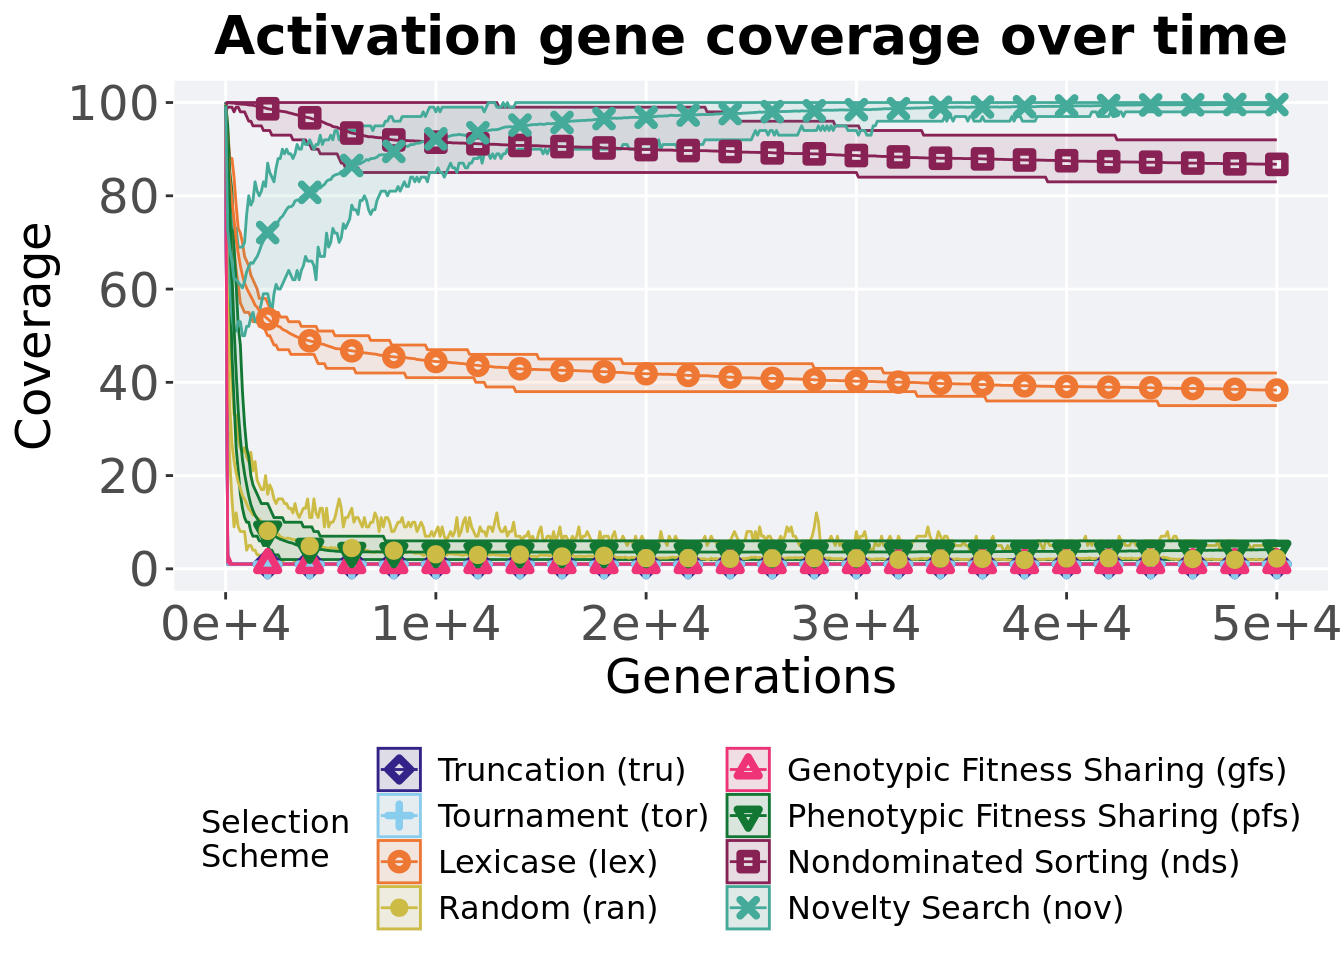
\includegraphics[width=1\linewidth]{base-diagnostics_files/figure-latex/con-act-ot-1}

\hypertarget{final-activation-gene-coverage}{%
\section{Final activation gene coverage}\label{final-activation-gene-coverage}}

Activation gene coverage found in the final population at 50,000 generations.

\begin{Shaded}
\begin{Highlighting}[]
\NormalTok{plot =}\StringTok{ }\KeywordTok{filter}\NormalTok{(over_time_df, gen }\OperatorTok{==}\StringTok{ }\DecValTok{50000}\NormalTok{) }\OperatorTok
\StringTok{  }\KeywordTok{ggplot}\NormalTok{(., }\KeywordTok{aes}\NormalTok{(}\DataTypeTok{x =}\NormalTok{ acro, }\DataTypeTok{y =}\NormalTok{ uni_str_pos, }\DataTypeTok{color =}\NormalTok{ acro, }\DataTypeTok{fill =}\NormalTok{ acro, }\DataTypeTok{shape =}\NormalTok{ acro)) }\OperatorTok{+}
\StringTok{  }\KeywordTok{geom_flat_violin}\NormalTok{(}\DataTypeTok{position =} \KeywordTok{position_nudge}\NormalTok{(}\DataTypeTok{x =} \FloatTok{.1}\NormalTok{, }\DataTypeTok{y =} \DecValTok{0}\NormalTok{), }\DataTypeTok{scale =} \StringTok{'width'}\NormalTok{, }\DataTypeTok{alpha =} \FloatTok{0.2}\NormalTok{, }\DataTypeTok{width =} \FloatTok{1.5}\NormalTok{) }\OperatorTok{+}
\StringTok{  }\KeywordTok{geom_boxplot}\NormalTok{(}\DataTypeTok{color =} \StringTok{'black'}\NormalTok{, }\DataTypeTok{width =} \FloatTok{.07}\NormalTok{, }\DataTypeTok{outlier.shape =} \OtherTok{NA}\NormalTok{, }\DataTypeTok{alpha =} \FloatTok{0.0}\NormalTok{, }\DataTypeTok{size =} \FloatTok{1.0}\NormalTok{, }\DataTypeTok{position =} \KeywordTok{position_nudge}\NormalTok{(}\DataTypeTok{x =} \FloatTok{.16}\NormalTok{, }\DataTypeTok{y =} \DecValTok{0}\NormalTok{)) }\OperatorTok{+}
\StringTok{  }\KeywordTok{geom_point}\NormalTok{(}\DataTypeTok{position =} \KeywordTok{position_jitter}\NormalTok{(}\DataTypeTok{width =} \FloatTok{0.03}\NormalTok{, }\DataTypeTok{height =} \FloatTok{0.02}\NormalTok{), }\DataTypeTok{size =} \FloatTok{2.0}\NormalTok{, }\DataTypeTok{alpha =} \FloatTok{1.0}\NormalTok{) }\OperatorTok{+}
\StringTok{  }\KeywordTok{scale_y_continuous}\NormalTok{(}
    \DataTypeTok{name=}\StringTok{"Coverage"}\NormalTok{,}
    \DataTypeTok{limits=}\KeywordTok{c}\NormalTok{(}\DecValTok{0}\NormalTok{, }\FloatTok{100.1}\NormalTok{),}
    \DataTypeTok{breaks=}\KeywordTok{seq}\NormalTok{(}\DecValTok{0}\NormalTok{,}\DecValTok{100}\NormalTok{, }\DecValTok{20}\NormalTok{),}
    \DataTypeTok{labels=}\KeywordTok{c}\NormalTok{(}\StringTok{"0"}\NormalTok{, }\StringTok{"20"}\NormalTok{, }\StringTok{"40"}\NormalTok{, }\StringTok{"60"}\NormalTok{, }\StringTok{"80"}\NormalTok{, }\StringTok{"100"}\NormalTok{)}
\NormalTok{  ) }\OperatorTok{+}
\StringTok{  }\KeywordTok{scale_x_discrete}\NormalTok{(}
    \DataTypeTok{name=}\StringTok{"Scheme"}
\NormalTok{  )}\OperatorTok{+}
\StringTok{  }\KeywordTok{scale_shape_manual}\NormalTok{(}\DataTypeTok{values=}\NormalTok{SHAPE)}\OperatorTok{+}
\StringTok{  }\KeywordTok{scale_colour_manual}\NormalTok{(}\DataTypeTok{values =}\NormalTok{ cb_palette, ) }\OperatorTok{+}
\StringTok{  }\KeywordTok{scale_fill_manual}\NormalTok{(}\DataTypeTok{values =}\NormalTok{ cb_palette) }\OperatorTok{+}
\StringTok{  }\KeywordTok{ggtitle}\NormalTok{(}\StringTok{'Final activation gene coverage'}\NormalTok{)}\OperatorTok{+}
\StringTok{  }\NormalTok{p_theme}

\KeywordTok{plot_grid}\NormalTok{(}
\NormalTok{  plot }\OperatorTok{+}
\StringTok{    }\KeywordTok{theme}\NormalTok{(}\DataTypeTok{legend.position=}\StringTok{"none"}\NormalTok{),}
\NormalTok{  legend,}
  \DataTypeTok{nrow=}\DecValTok{2}\NormalTok{,}
  \DataTypeTok{rel_heights =} \KeywordTok{c}\NormalTok{(}\DecValTok{3}\NormalTok{,}\DecValTok{1}\NormalTok{)}
\NormalTok{)}
\end{Highlighting}
\end{Shaded}

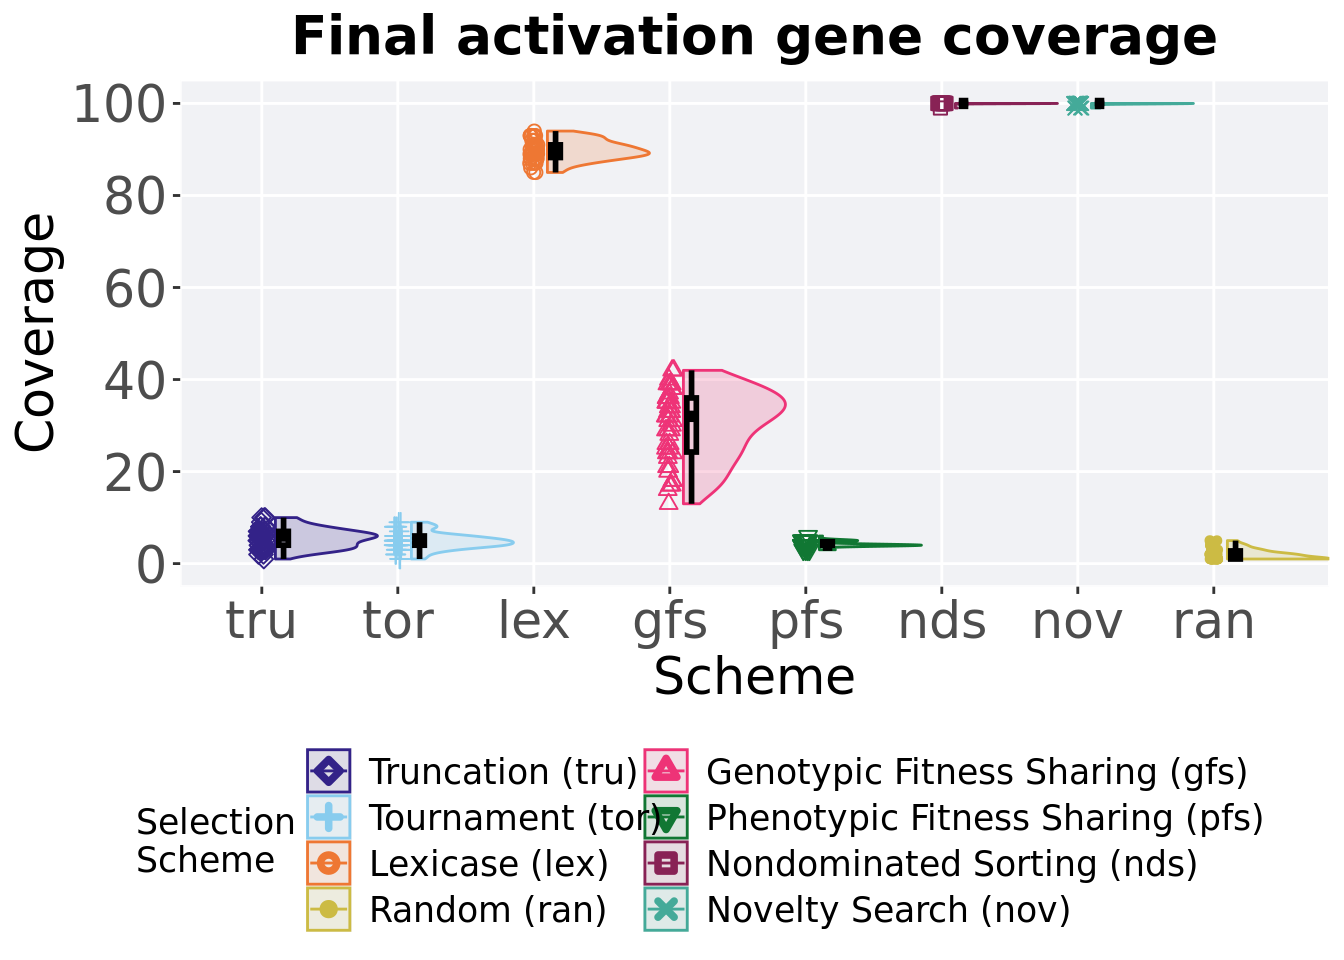
\includegraphics[width=1\linewidth]{base-diagnostics_files/figure-latex/con-act-end-1}

\hypertarget{stats-5}{%
\subsection{Stats}\label{stats-5}}

Summary statistics for the coverage found in the final population.

\begin{Shaded}
\begin{Highlighting}[]
\NormalTok{act_coverage =}\StringTok{ }\KeywordTok{filter}\NormalTok{(over_time_df, gen }\OperatorTok{==}\StringTok{ }\DecValTok{50000}\NormalTok{)}
\NormalTok{act_coverage}\OperatorTok{$}\NormalTok{acro =}\StringTok{ }\KeywordTok{factor}\NormalTok{(act_coverage}\OperatorTok{$}\NormalTok{acro, }\DataTypeTok{levels =} \KeywordTok{c}\NormalTok{(}\StringTok{'nov'}\NormalTok{,}\StringTok{'nds'}\NormalTok{,}\StringTok{'lex'}\NormalTok{,}\StringTok{'pfs'}\NormalTok{,}\StringTok{'ran'}\NormalTok{,}\StringTok{'gfs'}\NormalTok{,}\StringTok{'tor'}\NormalTok{,}\StringTok{'tru'}\NormalTok{))}
\NormalTok{act_coverage }\OperatorTok
\StringTok{  }\KeywordTok{group_by}\NormalTok{(acro) }\OperatorTok
\StringTok{  }\NormalTok{dplyr}\OperatorTok{::}\KeywordTok{summarise}\NormalTok{(}
    \DataTypeTok{count =} \KeywordTok{n}\NormalTok{(),}
    \DataTypeTok{na_cnt =} \KeywordTok{sum}\NormalTok{(}\KeywordTok{is.na}\NormalTok{(uni_str_pos)),}
    \DataTypeTok{min =} \KeywordTok{min}\NormalTok{(uni_str_pos, }\DataTypeTok{na.rm =} \OtherTok{TRUE}\NormalTok{),}
    \DataTypeTok{median =} \KeywordTok{median}\NormalTok{(uni_str_pos, }\DataTypeTok{na.rm =} \OtherTok{TRUE}\NormalTok{),}
    \DataTypeTok{mean =} \KeywordTok{mean}\NormalTok{(uni_str_pos, }\DataTypeTok{na.rm =} \OtherTok{TRUE}\NormalTok{),}
    \DataTypeTok{max =} \KeywordTok{max}\NormalTok{(uni_str_pos, }\DataTypeTok{na.rm =} \OtherTok{TRUE}\NormalTok{),}
    \DataTypeTok{IQR =} \KeywordTok{IQR}\NormalTok{(uni_str_pos, }\DataTypeTok{na.rm =} \OtherTok{TRUE}\NormalTok{)}
\NormalTok{  )}
\end{Highlighting}
\end{Shaded}

\begin{verbatim}
## # A tibble: 8 x 8
##   acro  count na_cnt   min median  mean   max   IQR
##   <fct> <int>  <int> <int>  <dbl> <dbl> <int> <dbl>
## 1 nov      50      0    98    100 99.6    100     1
## 2 nds      50      0    83     86 86.7     92     3
## 3 lex      50      0    35     38 38.3     42     1
## 4 pfs      50      0     2      4  4.12     6     2
## 5 ran      50      0     1      2  2.22     6     2
## 6 gfs      50      0     1      1  1        1     0
## 7 tor      50      0     1      1  1        1     0
## 8 tru      50      0     1      1  1        1     0
\end{verbatim}

Kruskal--Wallis test illustrates evidence of statistical differences.

\begin{Shaded}
\begin{Highlighting}[]
\KeywordTok{kruskal.test}\NormalTok{(uni_str_pos }\OperatorTok{~}\StringTok{ }\NormalTok{acro, }\DataTypeTok{data =}\NormalTok{ act_coverage)}
\end{Highlighting}
\end{Shaded}

\begin{verbatim}
## 
##  Kruskal-Wallis rank sum test
## 
## data:  uni_str_pos by acro
## Kruskal-Wallis chi-squared = 381.66, df = 7, p-value < 2.2e-16
\end{verbatim}

Results for post-hoc Wilcoxon rank-sum test with a Bonferroni correction.

\begin{Shaded}
\begin{Highlighting}[]
\KeywordTok{pairwise.wilcox.test}\NormalTok{(}\DataTypeTok{x =}\NormalTok{ act_coverage}\OperatorTok{$}\NormalTok{uni_str_pos, }\DataTypeTok{g =}\NormalTok{ act_coverage}\OperatorTok{$}\NormalTok{acro, }\DataTypeTok{p.adjust.method =} \StringTok{"bonferroni"}\NormalTok{,}
                     \DataTypeTok{paired =} \OtherTok{FALSE}\NormalTok{, }\DataTypeTok{conf.int =} \OtherTok{FALSE}\NormalTok{, }\DataTypeTok{alternative =} \StringTok{'l'}\NormalTok{)}
\end{Highlighting}
\end{Shaded}

\begin{verbatim}
## 
##  Pairwise comparisons using Wilcoxon rank sum test with continuity correction 
## 
## data:  act_coverage$uni_str_pos and act_coverage$acro 
## 
##     nov     nds     lex     pfs     ran     gfs tor
## nds < 2e-16 -       -       -       -       -   -  
## lex < 2e-16 < 2e-16 -       -       -       -   -  
## pfs < 2e-16 < 2e-16 < 2e-16 -       -       -   -  
## ran < 2e-16 < 2e-16 < 2e-16 7.1e-09 -       -   -  
## gfs < 2e-16 < 2e-16 < 2e-16 < 2e-16 6.0e-09 -   -  
## tor < 2e-16 < 2e-16 < 2e-16 < 2e-16 6.0e-09 1   -  
## tru < 2e-16 < 2e-16 < 2e-16 < 2e-16 6.0e-09 1   1  
## 
## P value adjustment method: bonferroni
\end{verbatim}

\hypertarget{satisfactory-trait-coverage-over-time}{%
\section{Satisfactory trait coverage over time}\label{satisfactory-trait-coverage-over-time}}

Satisfactory trait coverage in a population over time.
Data points on the graph is the average activation gene coverage across 50 replicates every 2000 generations.
Shading comes from the best and worse coverage across 50 replicates.

\begin{Shaded}
\begin{Highlighting}[]
\NormalTok{lines =}\StringTok{ }\NormalTok{over_time_df }\OperatorTok
\StringTok{  }\KeywordTok{group_by}\NormalTok{(scheme, gen) }\OperatorTok
\StringTok{  }\NormalTok{dplyr}\OperatorTok{::}\KeywordTok{summarise}\NormalTok{(}
    \DataTypeTok{min =} \KeywordTok{min}\NormalTok{(pop_uni_obj),}
    \DataTypeTok{mean =} \KeywordTok{mean}\NormalTok{(pop_uni_obj),}
    \DataTypeTok{max =} \KeywordTok{max}\NormalTok{(pop_uni_obj)}
\NormalTok{  )}
\end{Highlighting}
\end{Shaded}

\begin{verbatim}
## `summarise()` has grouped output by 'scheme'. You can override using the
## `.groups` argument.
\end{verbatim}

\begin{Shaded}
\begin{Highlighting}[]
\NormalTok{lines}\OperatorTok{$}\NormalTok{scheme <-}\StringTok{ }\KeywordTok{factor}\NormalTok{(lines}\OperatorTok{$}\NormalTok{scheme, }\DataTypeTok{levels =} \KeywordTok{c}\NormalTok{(}\StringTok{'Truncation (tru)'}\NormalTok{,}\StringTok{'Tournament (tor)'}\NormalTok{,}\StringTok{'Lexicase (lex)'}\NormalTok{,}\StringTok{'Random (ran)'}\NormalTok{,}\StringTok{'Genotypic Fitness Sharing (gfs)'}\NormalTok{,}\StringTok{'Phenotypic Fitness Sharing (pfs)'}\NormalTok{,}\StringTok{'Nondominated Sorting (nds)'}\NormalTok{,}\StringTok{'Novelty Search (nov)'}\NormalTok{))}

\NormalTok{over_time_plot =}\StringTok{ }\KeywordTok{ggplot}\NormalTok{(lines, }\KeywordTok{aes}\NormalTok{(}\DataTypeTok{x=}\NormalTok{gen, }\DataTypeTok{y=}\NormalTok{mean, }\DataTypeTok{group =}\NormalTok{ scheme, }\DataTypeTok{fill =}\NormalTok{ scheme, }\DataTypeTok{color =}\NormalTok{ scheme, }\DataTypeTok{shape =}\NormalTok{ scheme)) }\OperatorTok{+}
\StringTok{  }\KeywordTok{geom_ribbon}\NormalTok{(}\KeywordTok{aes}\NormalTok{(}\DataTypeTok{ymin =}\NormalTok{ min, }\DataTypeTok{ymax =}\NormalTok{ max), }\DataTypeTok{alpha =} \FloatTok{0.1}\NormalTok{) }\OperatorTok{+}
\StringTok{  }\KeywordTok{geom_line}\NormalTok{(}\DataTypeTok{size =} \FloatTok{0.5}\NormalTok{) }\OperatorTok{+}
\StringTok{  }\KeywordTok{geom_point}\NormalTok{(}\DataTypeTok{data =} \KeywordTok{filter}\NormalTok{(lines, gen }\OperatorTok\StringTok{ }\DecValTok{2000} \OperatorTok{==}\StringTok{ }\DecValTok{0} \OperatorTok{&}\StringTok{ }\NormalTok{gen }\OperatorTok{!=}\StringTok{ }\DecValTok{0}\NormalTok{), }\DataTypeTok{size =} \FloatTok{1.5}\NormalTok{, }\DataTypeTok{stroke =} \FloatTok{2.0}\NormalTok{, }\DataTypeTok{alpha =} \FloatTok{1.0}\NormalTok{) }\OperatorTok{+}
\StringTok{  }\KeywordTok{scale_y_continuous}\NormalTok{(}
    \DataTypeTok{name=}\StringTok{"Coverage"}\NormalTok{,}
    \DataTypeTok{limits=}\KeywordTok{c}\NormalTok{(}\DecValTok{0}\NormalTok{, }\DecValTok{100}\NormalTok{),}
    \DataTypeTok{breaks=}\KeywordTok{seq}\NormalTok{(}\DecValTok{0}\NormalTok{,}\DecValTok{100}\NormalTok{, }\DecValTok{20}\NormalTok{),}
    \DataTypeTok{labels=}\KeywordTok{c}\NormalTok{(}\StringTok{"0"}\NormalTok{, }\StringTok{"20"}\NormalTok{, }\StringTok{"40"}\NormalTok{, }\StringTok{"60"}\NormalTok{, }\StringTok{"80"}\NormalTok{, }\StringTok{"100"}\NormalTok{)}
\NormalTok{  ) }\OperatorTok{+}
\StringTok{  }\KeywordTok{scale_x_continuous}\NormalTok{(}
    \DataTypeTok{name=}\StringTok{"Generations"}\NormalTok{,}
    \DataTypeTok{limits=}\KeywordTok{c}\NormalTok{(}\DecValTok{0}\NormalTok{, }\DecValTok{50000}\NormalTok{),}
    \DataTypeTok{breaks=}\KeywordTok{c}\NormalTok{(}\DecValTok{0}\NormalTok{, }\DecValTok{10000}\NormalTok{, }\DecValTok{20000}\NormalTok{, }\DecValTok{30000}\NormalTok{, }\DecValTok{40000}\NormalTok{, }\DecValTok{50000}\NormalTok{),}
    \DataTypeTok{labels=}\KeywordTok{c}\NormalTok{(}\StringTok{"0e+4"}\NormalTok{, }\StringTok{"1e+4"}\NormalTok{, }\StringTok{"2e+4"}\NormalTok{, }\StringTok{"3e+4"}\NormalTok{, }\StringTok{"4e+4"}\NormalTok{, }\StringTok{"5e+4"}\NormalTok{)}

\NormalTok{  ) }\OperatorTok{+}
\StringTok{  }\KeywordTok{scale_shape_manual}\NormalTok{(}\DataTypeTok{values=}\KeywordTok{c}\NormalTok{(}\DecValTok{5}\NormalTok{,}\DecValTok{3}\NormalTok{,}\DecValTok{1}\NormalTok{,}\DecValTok{20}\NormalTok{,}\DecValTok{2}\NormalTok{,}\DecValTok{6}\NormalTok{,}\DecValTok{0}\NormalTok{,}\DecValTok{4}\NormalTok{))}\OperatorTok{+}
\StringTok{  }\KeywordTok{scale_colour_manual}\NormalTok{(}\DataTypeTok{values =} \KeywordTok{c}\NormalTok{(}\StringTok{'#332288'}\NormalTok{,}\StringTok{'#88CCEE'}\NormalTok{,}\StringTok{'#EE7733'}\NormalTok{,}\StringTok{'#CCBB44'}\NormalTok{,}\StringTok{'#EE3377'}\NormalTok{,}\StringTok{'#117733'}\NormalTok{,}\StringTok{'#882255'}\NormalTok{,}\StringTok{'#44AA99'}\NormalTok{)) }\OperatorTok{+}
\StringTok{  }\KeywordTok{scale_fill_manual}\NormalTok{(}\DataTypeTok{values =} \KeywordTok{c}\NormalTok{(}\StringTok{'#332288'}\NormalTok{,}\StringTok{'#88CCEE'}\NormalTok{,}\StringTok{'#EE7733'}\NormalTok{,}\StringTok{'#CCBB44'}\NormalTok{,}\StringTok{'#EE3377'}\NormalTok{,}\StringTok{'#117733'}\NormalTok{,}\StringTok{'#882255'}\NormalTok{,}\StringTok{'#44AA99'}\NormalTok{)) }\OperatorTok{+}
\StringTok{  }\KeywordTok{ggtitle}\NormalTok{(}\StringTok{'Satisfactory trait coverage over time'}\NormalTok{)}\OperatorTok{+}
\StringTok{  }\NormalTok{p_theme }\OperatorTok{+}
\StringTok{  }\KeywordTok{guides}\NormalTok{(}
    \DataTypeTok{shape=}\KeywordTok{guide_legend}\NormalTok{(}\DataTypeTok{ncol=}\DecValTok{2}\NormalTok{, }\DataTypeTok{title.position =} \StringTok{"left"}\NormalTok{, }\DataTypeTok{title =} \StringTok{'Selection }\CharTok{\textbackslash{}n}\StringTok{Scheme'}\NormalTok{),}
    \DataTypeTok{color=}\KeywordTok{guide_legend}\NormalTok{(}\DataTypeTok{ncol=}\DecValTok{2}\NormalTok{, }\DataTypeTok{title.position =} \StringTok{"left"}\NormalTok{, }\DataTypeTok{title =} \StringTok{'Selection }\CharTok{\textbackslash{}n}\StringTok{Scheme'}\NormalTok{),}
    \DataTypeTok{fill=}\KeywordTok{guide_legend}\NormalTok{(}\DataTypeTok{ncol=}\DecValTok{2}\NormalTok{, }\DataTypeTok{title.position =} \StringTok{"left"}\NormalTok{, }\DataTypeTok{title =} \StringTok{'Selection }\CharTok{\textbackslash{}n}\StringTok{Scheme'}\NormalTok{)}
\NormalTok{  )}

\NormalTok{over_time_plot}
\end{Highlighting}
\end{Shaded}

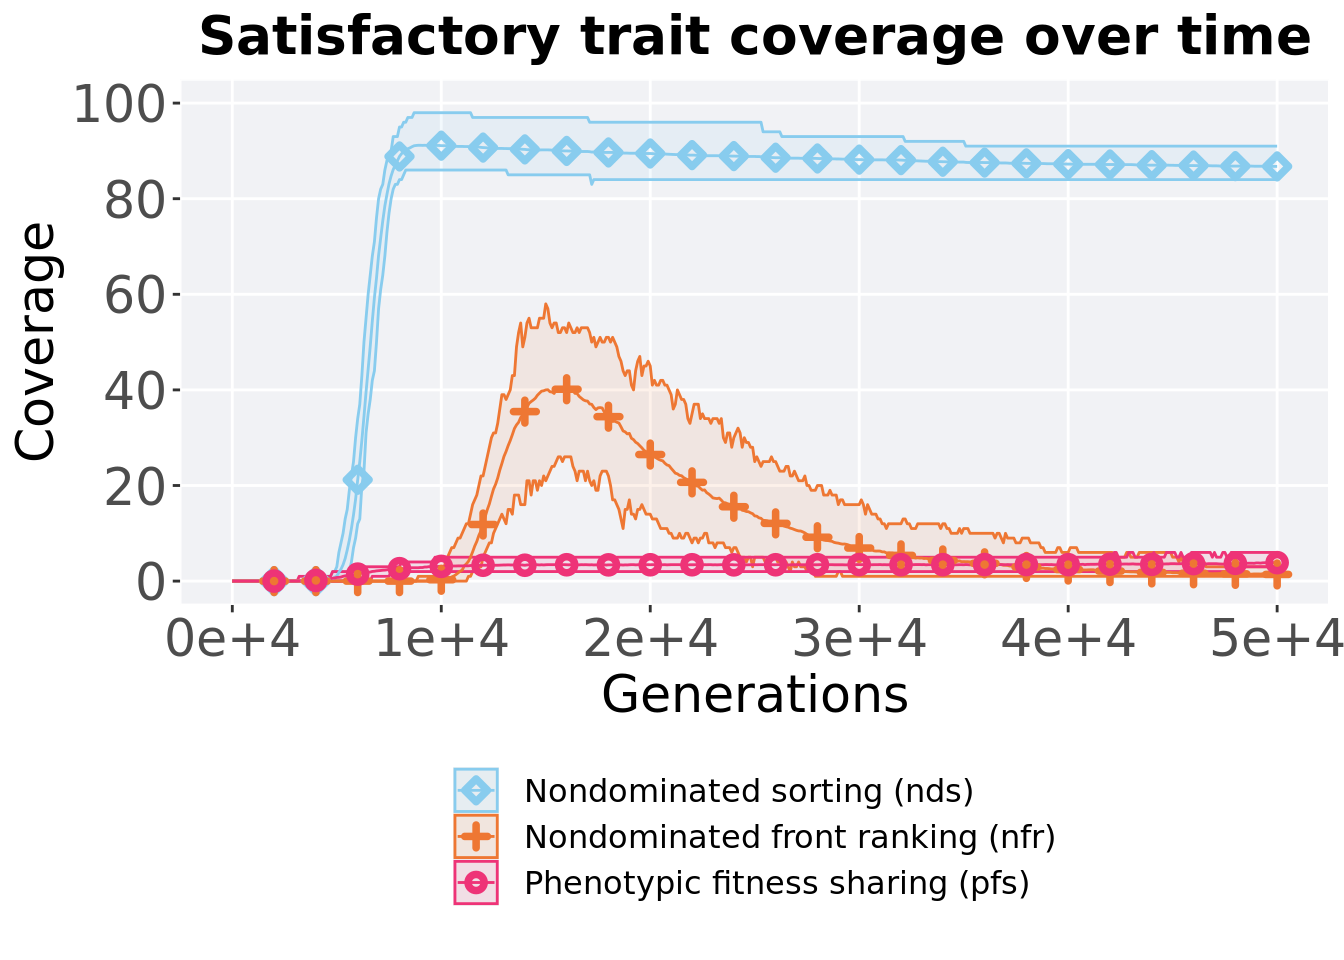
\includegraphics[width=1\linewidth]{base-diagnostics_files/figure-latex/con-sat-ot-1}

\hypertarget{final-satisfactory-trait-coverage}{%
\section{Final satisfactory trait coverage}\label{final-satisfactory-trait-coverage}}

Satisfactory trait coverage found in the final population at 50,000 generations.

\begin{Shaded}
\begin{Highlighting}[]
\NormalTok{plot =}\StringTok{ }\KeywordTok{filter}\NormalTok{(over_time_df, gen }\OperatorTok{==}\StringTok{ }\DecValTok{50000}\NormalTok{) }\OperatorTok
\StringTok{  }\KeywordTok{ggplot}\NormalTok{(., }\KeywordTok{aes}\NormalTok{(}\DataTypeTok{x =}\NormalTok{ acro, }\DataTypeTok{y =}\NormalTok{ pop_uni_obj, }\DataTypeTok{color =}\NormalTok{ acro, }\DataTypeTok{fill =}\NormalTok{ acro, }\DataTypeTok{shape =}\NormalTok{ acro)) }\OperatorTok{+}
\StringTok{  }\KeywordTok{geom_flat_violin}\NormalTok{(}\DataTypeTok{position =} \KeywordTok{position_nudge}\NormalTok{(}\DataTypeTok{x =} \FloatTok{.1}\NormalTok{, }\DataTypeTok{y =} \DecValTok{0}\NormalTok{), }\DataTypeTok{scale =} \StringTok{'width'}\NormalTok{, }\DataTypeTok{alpha =} \FloatTok{0.2}\NormalTok{, }\DataTypeTok{width =} \FloatTok{1.5}\NormalTok{) }\OperatorTok{+}
\StringTok{  }\KeywordTok{geom_boxplot}\NormalTok{(}\DataTypeTok{color =} \StringTok{'black'}\NormalTok{, }\DataTypeTok{width =} \FloatTok{.07}\NormalTok{, }\DataTypeTok{outlier.shape =} \OtherTok{NA}\NormalTok{, }\DataTypeTok{alpha =} \FloatTok{0.0}\NormalTok{, }\DataTypeTok{size =} \FloatTok{1.0}\NormalTok{, }\DataTypeTok{position =} \KeywordTok{position_nudge}\NormalTok{(}\DataTypeTok{x =} \FloatTok{.16}\NormalTok{, }\DataTypeTok{y =} \DecValTok{0}\NormalTok{)) }\OperatorTok{+}
\StringTok{  }\KeywordTok{geom_point}\NormalTok{(}\DataTypeTok{position =} \KeywordTok{position_jitter}\NormalTok{(}\DataTypeTok{width =} \FloatTok{0.03}\NormalTok{, }\DataTypeTok{height =} \FloatTok{0.02}\NormalTok{), }\DataTypeTok{size =} \FloatTok{2.0}\NormalTok{, }\DataTypeTok{alpha =} \FloatTok{1.0}\NormalTok{) }\OperatorTok{+}
\StringTok{  }\KeywordTok{scale_y_continuous}\NormalTok{(}
    \DataTypeTok{name=}\StringTok{"Coverage"}\NormalTok{,}
    \DataTypeTok{limits=}\KeywordTok{c}\NormalTok{(}\OperatorTok{-}\FloatTok{0.1}\NormalTok{, }\DecValTok{100}\NormalTok{),}
    \DataTypeTok{breaks=}\KeywordTok{seq}\NormalTok{(}\DecValTok{0}\NormalTok{,}\DecValTok{100}\NormalTok{, }\DecValTok{20}\NormalTok{),}
    \DataTypeTok{labels=}\KeywordTok{c}\NormalTok{(}\StringTok{"0"}\NormalTok{, }\StringTok{"20"}\NormalTok{, }\StringTok{"40"}\NormalTok{, }\StringTok{"60"}\NormalTok{, }\StringTok{"80"}\NormalTok{, }\StringTok{"100"}\NormalTok{)}
\NormalTok{  ) }\OperatorTok{+}
\StringTok{  }\KeywordTok{scale_x_discrete}\NormalTok{(}
    \DataTypeTok{name=}\StringTok{"Scheme"}
\NormalTok{  )}\OperatorTok{+}
\StringTok{  }\KeywordTok{scale_shape_manual}\NormalTok{(}\DataTypeTok{values=}\NormalTok{SHAPE)}\OperatorTok{+}
\StringTok{  }\KeywordTok{scale_colour_manual}\NormalTok{(}\DataTypeTok{values =}\NormalTok{ cb_palette, ) }\OperatorTok{+}
\StringTok{  }\KeywordTok{scale_fill_manual}\NormalTok{(}\DataTypeTok{values =}\NormalTok{ cb_palette) }\OperatorTok{+}
\StringTok{  }\KeywordTok{ggtitle}\NormalTok{(}\StringTok{'Final satisfactory trait coverage'}\NormalTok{)}\OperatorTok{+}
\StringTok{  }\NormalTok{p_theme}

\KeywordTok{plot_grid}\NormalTok{(}
\NormalTok{  plot }\OperatorTok{+}
\StringTok{    }\KeywordTok{theme}\NormalTok{(}\DataTypeTok{legend.position=}\StringTok{"none"}\NormalTok{),}
\NormalTok{  legend,}
  \DataTypeTok{nrow=}\DecValTok{2}\NormalTok{,}
  \DataTypeTok{rel_heights =} \KeywordTok{c}\NormalTok{(}\DecValTok{3}\NormalTok{,}\DecValTok{1}\NormalTok{)}
\NormalTok{)}
\end{Highlighting}
\end{Shaded}

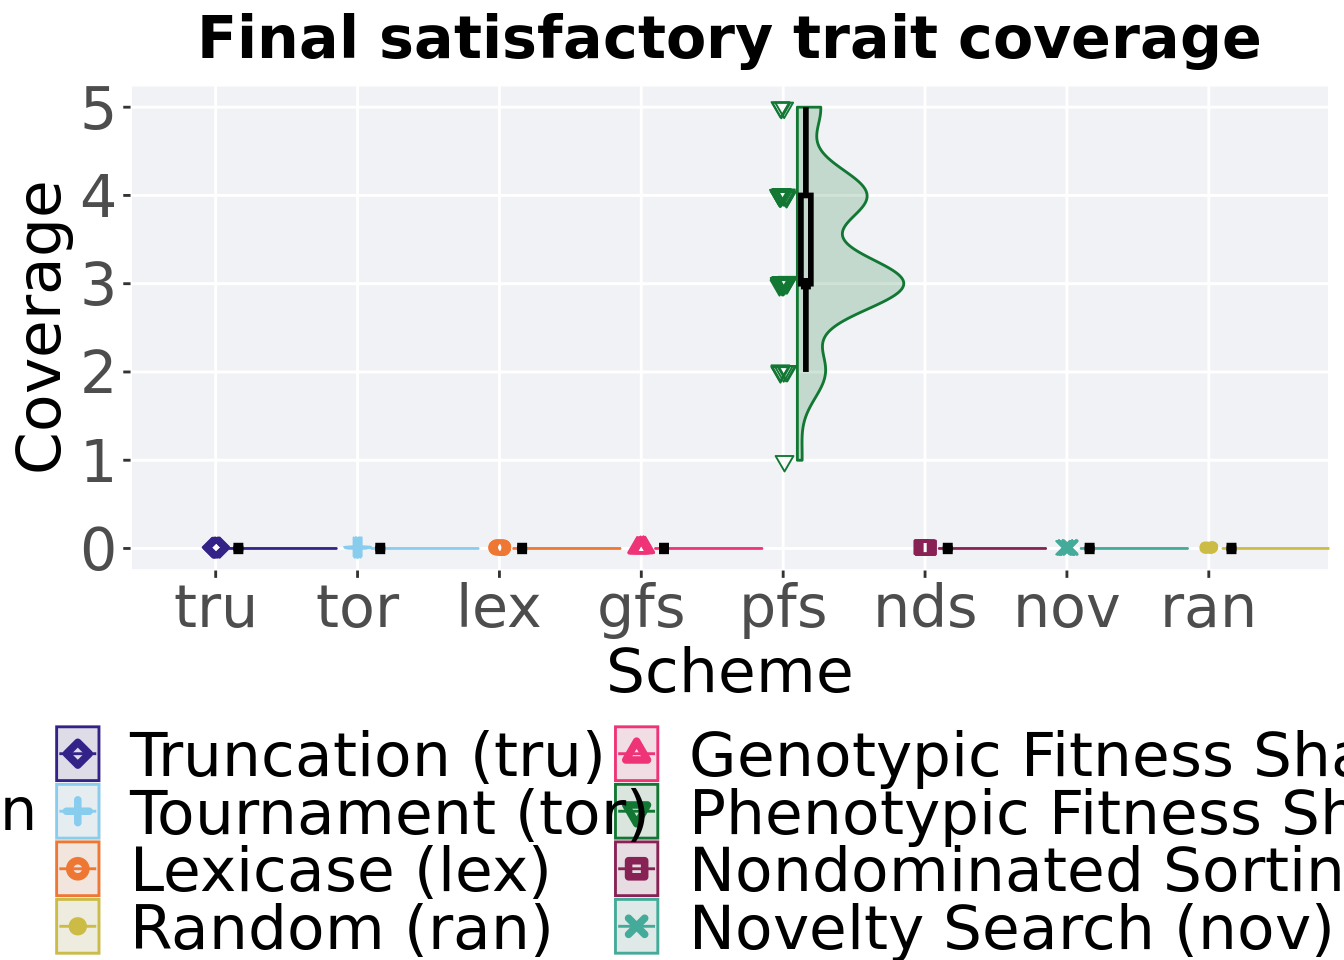
\includegraphics[width=1\linewidth]{base-diagnostics_files/figure-latex/con-sat-end-1}

\hypertarget{stats-6}{%
\subsection{Stats}\label{stats-6}}

Summary statistics for the coverage found in the final population.

\begin{Shaded}
\begin{Highlighting}[]
\NormalTok{sat_coverage =}\StringTok{ }\KeywordTok{filter}\NormalTok{(over_time_df, gen }\OperatorTok{==}\StringTok{ }\DecValTok{50000}\NormalTok{)}
\NormalTok{sat_coverage}\OperatorTok{$}\NormalTok{acro =}\StringTok{ }\KeywordTok{factor}\NormalTok{(sat_coverage}\OperatorTok{$}\NormalTok{acro, }\DataTypeTok{levels =} \KeywordTok{c}\NormalTok{(}\StringTok{'nds'}\NormalTok{,}\StringTok{'lex'}\NormalTok{,}\StringTok{'pfs'}\NormalTok{,}\StringTok{'gfs'}\NormalTok{,}\StringTok{'tor'}\NormalTok{,}\StringTok{'tru'}\NormalTok{,}\StringTok{'nov'}\NormalTok{,}\StringTok{'ran'}\NormalTok{))}
\NormalTok{sat_coverage }\OperatorTok
\StringTok{  }\KeywordTok{group_by}\NormalTok{(acro) }\OperatorTok
\StringTok{  }\NormalTok{dplyr}\OperatorTok{::}\KeywordTok{summarise}\NormalTok{(}
    \DataTypeTok{count =} \KeywordTok{n}\NormalTok{(),}
    \DataTypeTok{na_cnt =} \KeywordTok{sum}\NormalTok{(}\KeywordTok{is.na}\NormalTok{(pop_uni_obj)),}
    \DataTypeTok{min =} \KeywordTok{min}\NormalTok{(pop_uni_obj, }\DataTypeTok{na.rm =} \OtherTok{TRUE}\NormalTok{),}
    \DataTypeTok{median =} \KeywordTok{median}\NormalTok{(pop_uni_obj, }\DataTypeTok{na.rm =} \OtherTok{TRUE}\NormalTok{),}
    \DataTypeTok{mean =} \KeywordTok{mean}\NormalTok{(pop_uni_obj, }\DataTypeTok{na.rm =} \OtherTok{TRUE}\NormalTok{),}
    \DataTypeTok{max =} \KeywordTok{max}\NormalTok{(pop_uni_obj, }\DataTypeTok{na.rm =} \OtherTok{TRUE}\NormalTok{),}
    \DataTypeTok{IQR =} \KeywordTok{IQR}\NormalTok{(pop_uni_obj, }\DataTypeTok{na.rm =} \OtherTok{TRUE}\NormalTok{)}
\NormalTok{  )}
\end{Highlighting}
\end{Shaded}

\begin{verbatim}
## # A tibble: 8 x 8
##   acro  count na_cnt   min median  mean   max   IQR
##   <fct> <int>  <int> <int>  <dbl> <dbl> <int> <dbl>
## 1 nds      50      0    83     86 86.7     92     3
## 2 lex      50      0    35     38 38.3     42     1
## 3 pfs      50      0     2      4  3.88     6     2
## 4 gfs      50      0     1      1  1        1     0
## 5 tor      50      0     1      1  1        1     0
## 6 tru      50      0     1      1  1        1     0
## 7 nov      50      0     0      0  0        0     0
## 8 ran      50      0     0      0  0        0     0
\end{verbatim}

Kruskal--Wallis test illustrates evidence of statistical differences.

\begin{Shaded}
\begin{Highlighting}[]
\KeywordTok{kruskal.test}\NormalTok{(pop_uni_obj }\OperatorTok{~}\StringTok{ }\NormalTok{acro, }\DataTypeTok{data =}\NormalTok{ sat_coverage)}
\end{Highlighting}
\end{Shaded}

\begin{verbatim}
## 
##  Kruskal-Wallis rank sum test
## 
## data:  pop_uni_obj by acro
## Kruskal-Wallis chi-squared = 396.63, df = 7, p-value < 2.2e-16
\end{verbatim}

Results for post-hoc Wilcoxon rank-sum test with a Bonferroni correction.

\begin{Shaded}
\begin{Highlighting}[]
\KeywordTok{pairwise.wilcox.test}\NormalTok{(}\DataTypeTok{x =}\NormalTok{ sat_coverage}\OperatorTok{$}\NormalTok{pop_uni_obj, }\DataTypeTok{g =}\NormalTok{ sat_coverage}\OperatorTok{$}\NormalTok{acro, }\DataTypeTok{p.adjust.method =} \StringTok{"bonferroni"}\NormalTok{,}
                     \DataTypeTok{paired =} \OtherTok{FALSE}\NormalTok{, }\DataTypeTok{conf.int =} \OtherTok{FALSE}\NormalTok{, }\DataTypeTok{alternative =} \StringTok{'l'}\NormalTok{)}
\end{Highlighting}
\end{Shaded}

\begin{verbatim}
## 
##  Pairwise comparisons using Wilcoxon rank sum test with continuity correction 
## 
## data:  sat_coverage$pop_uni_obj and sat_coverage$acro 
## 
##     nds    lex    pfs    gfs    tor    tru    nov
## lex <2e-16 -      -      -      -      -      -  
## pfs <2e-16 <2e-16 -      -      -      -      -  
## gfs <2e-16 <2e-16 <2e-16 -      -      -      -  
## tor <2e-16 <2e-16 <2e-16 1      -      -      -  
## tru <2e-16 <2e-16 <2e-16 1      1      -      -  
## nov <2e-16 <2e-16 <2e-16 <2e-16 <2e-16 <2e-16 -  
## ran <2e-16 <2e-16 <2e-16 <2e-16 <2e-16 <2e-16 1  
## 
## P value adjustment method: bonferroni
\end{verbatim}

\hypertarget{multi-path-exploration-results}{%
\chapter{Multi-path exploration results}\label{multi-path-exploration-results}}

Here we present the results for \textbf{best performances} and \textbf{activation gene coverage} found by each selection scheme on the multi-path exploration diagnostic.
50 replicates are conducted for each scheme explored.

\hypertarget{data-setup-3}{%
\section{Data setup}\label{data-setup-3}}

\begin{Shaded}
\begin{Highlighting}[]
\NormalTok{DIR =}\StringTok{ }\KeywordTok{paste}\NormalTok{(DATA_DIR,}\StringTok{'MULTIPATH_EXPLORATION/'}\NormalTok{, }\DataTypeTok{sep =} \StringTok{""}\NormalTok{, }\DataTypeTok{collapse =} \OtherTok{NULL}\NormalTok{)}
\NormalTok{over_time_df <-}\StringTok{ }\KeywordTok{read.csv}\NormalTok{(}\KeywordTok{paste}\NormalTok{(DIR,}\StringTok{'over-time.csv'}\NormalTok{, }\DataTypeTok{sep =} \StringTok{""}\NormalTok{, }\DataTypeTok{collapse =} \OtherTok{NULL}\NormalTok{), }\DataTypeTok{header =} \OtherTok{TRUE}\NormalTok{, }\DataTypeTok{stringsAsFactors =} \OtherTok{FALSE}\NormalTok{)}
\NormalTok{over_time_df}\OperatorTok{$}\NormalTok{uni_str_pos =}\StringTok{ }\NormalTok{over_time_df}\OperatorTok{$}\NormalTok{uni_str_pos }\OperatorTok{+}\StringTok{ }\NormalTok{over_time_df}\OperatorTok{$}\NormalTok{arc_acti_gene }\OperatorTok{-}\StringTok{ }\NormalTok{over_time_df}\OperatorTok{$}\NormalTok{overlap}
\NormalTok{over_time_df}\OperatorTok{$}\NormalTok{scheme <-}\StringTok{ }\KeywordTok{factor}\NormalTok{(over_time_df}\OperatorTok{$}\NormalTok{scheme, }\DataTypeTok{levels =}\NormalTok{ NAMES)}
\NormalTok{over_time_df}\OperatorTok{$}\NormalTok{acro <-}\StringTok{ }\KeywordTok{factor}\NormalTok{(over_time_df}\OperatorTok{$}\NormalTok{acro, }\DataTypeTok{levels =}\NormalTok{ ACRO)}

\NormalTok{best_df <-}\StringTok{ }\KeywordTok{read.csv}\NormalTok{(}\KeywordTok{paste}\NormalTok{(DIR,}\StringTok{'best.csv'}\NormalTok{, }\DataTypeTok{sep =} \StringTok{""}\NormalTok{, }\DataTypeTok{collapse =} \OtherTok{NULL}\NormalTok{), }\DataTypeTok{header =} \OtherTok{TRUE}\NormalTok{, }\DataTypeTok{stringsAsFactors =} \OtherTok{FALSE}\NormalTok{)}
\NormalTok{best_df}\OperatorTok{$}\NormalTok{acro <-}\StringTok{ }\KeywordTok{factor}\NormalTok{(best_df}\OperatorTok{$}\NormalTok{acro, }\DataTypeTok{levels =}\NormalTok{ ACRO)}
\end{Highlighting}
\end{Shaded}

\hypertarget{activation-gene-coverage-over-time-1}{%
\section{Activation gene coverage over time}\label{activation-gene-coverage-over-time-1}}

Activation gene coverage in a population over time.
Data points on the graph is the average activation gene coverage across 50 replicates every 2000 generations.
Shading comes from the best and worse coverage across 50 replicates.

\begin{Shaded}
\begin{Highlighting}[]
\NormalTok{lines =}\StringTok{ }\NormalTok{over_time_df }\OperatorTok
\StringTok{  }\KeywordTok{group_by}\NormalTok{(scheme, gen) }\OperatorTok
\StringTok{  }\NormalTok{dplyr}\OperatorTok{::}\KeywordTok{summarise}\NormalTok{(}
    \DataTypeTok{min =} \KeywordTok{min}\NormalTok{(uni_str_pos),}
    \DataTypeTok{mean =} \KeywordTok{mean}\NormalTok{(uni_str_pos),}
    \DataTypeTok{max =} \KeywordTok{max}\NormalTok{(uni_str_pos)}
\NormalTok{  )}
\end{Highlighting}
\end{Shaded}

\begin{verbatim}
## `summarise()` has grouped output by 'scheme'. You can override using the
## `.groups` argument.
\end{verbatim}

\begin{Shaded}
\begin{Highlighting}[]
\NormalTok{lines}\OperatorTok{$}\NormalTok{scheme <-}\StringTok{ }\KeywordTok{factor}\NormalTok{(lines}\OperatorTok{$}\NormalTok{scheme, }\DataTypeTok{levels =} \KeywordTok{c}\NormalTok{(}\StringTok{'Truncation (tru)'}\NormalTok{,}\StringTok{'Tournament (tor)'}\NormalTok{,}\StringTok{'Lexicase (lex)'}\NormalTok{,}\StringTok{'Random (ran)'}\NormalTok{,}\StringTok{'Genotypic Fitness Sharing (gfs)'}\NormalTok{,}\StringTok{'Phenotypic Fitness Sharing (pfs)'}\NormalTok{,}\StringTok{'Nondominated Sorting (nds)'}\NormalTok{,}\StringTok{'Novelty Search (nov)'}\NormalTok{))}

\NormalTok{over_time_plot =}\StringTok{ }\KeywordTok{ggplot}\NormalTok{(lines, }\KeywordTok{aes}\NormalTok{(}\DataTypeTok{x=}\NormalTok{gen, }\DataTypeTok{y=}\NormalTok{mean, }\DataTypeTok{group =}\NormalTok{ scheme, }\DataTypeTok{fill =}\NormalTok{ scheme, }\DataTypeTok{color =}\NormalTok{ scheme, }\DataTypeTok{shape =}\NormalTok{ scheme)) }\OperatorTok{+}
\StringTok{  }\KeywordTok{geom_ribbon}\NormalTok{(}\KeywordTok{aes}\NormalTok{(}\DataTypeTok{ymin =}\NormalTok{ min, }\DataTypeTok{ymax =}\NormalTok{ max), }\DataTypeTok{alpha =} \FloatTok{0.1}\NormalTok{) }\OperatorTok{+}
\StringTok{  }\KeywordTok{geom_line}\NormalTok{(}\DataTypeTok{size =} \FloatTok{0.5}\NormalTok{) }\OperatorTok{+}
\StringTok{  }\KeywordTok{geom_point}\NormalTok{(}\DataTypeTok{data =} \KeywordTok{filter}\NormalTok{(lines, gen }\OperatorTok\StringTok{ }\DecValTok{2000} \OperatorTok{==}\StringTok{ }\DecValTok{0} \OperatorTok{&}\StringTok{ }\NormalTok{gen }\OperatorTok{!=}\StringTok{ }\DecValTok{0}\NormalTok{), }\DataTypeTok{size =} \FloatTok{1.5}\NormalTok{, }\DataTypeTok{stroke =} \FloatTok{2.0}\NormalTok{, }\DataTypeTok{alpha =} \FloatTok{1.0}\NormalTok{) }\OperatorTok{+}
\StringTok{  }\KeywordTok{scale_y_continuous}\NormalTok{(}
    \DataTypeTok{name=}\StringTok{"Coverage"}\NormalTok{,}
    \DataTypeTok{limits=}\KeywordTok{c}\NormalTok{(}\DecValTok{0}\NormalTok{, }\DecValTok{100}\NormalTok{),}
    \DataTypeTok{breaks=}\KeywordTok{seq}\NormalTok{(}\DecValTok{0}\NormalTok{,}\DecValTok{100}\NormalTok{, }\DecValTok{20}\NormalTok{),}
    \DataTypeTok{labels=}\KeywordTok{c}\NormalTok{(}\StringTok{"0"}\NormalTok{, }\StringTok{"20"}\NormalTok{, }\StringTok{"40"}\NormalTok{, }\StringTok{"60"}\NormalTok{, }\StringTok{"80"}\NormalTok{, }\StringTok{"100"}\NormalTok{)}
\NormalTok{  ) }\OperatorTok{+}
\StringTok{  }\KeywordTok{scale_x_continuous}\NormalTok{(}
    \DataTypeTok{name=}\StringTok{"Generations"}\NormalTok{,}
    \DataTypeTok{limits=}\KeywordTok{c}\NormalTok{(}\DecValTok{0}\NormalTok{, }\DecValTok{50000}\NormalTok{),}
    \DataTypeTok{breaks=}\KeywordTok{c}\NormalTok{(}\DecValTok{0}\NormalTok{, }\DecValTok{10000}\NormalTok{, }\DecValTok{20000}\NormalTok{, }\DecValTok{30000}\NormalTok{, }\DecValTok{40000}\NormalTok{, }\DecValTok{50000}\NormalTok{),}
    \DataTypeTok{labels=}\KeywordTok{c}\NormalTok{(}\StringTok{"0e+4"}\NormalTok{, }\StringTok{"1e+4"}\NormalTok{, }\StringTok{"2e+4"}\NormalTok{, }\StringTok{"3e+4"}\NormalTok{, }\StringTok{"4e+4"}\NormalTok{, }\StringTok{"5e+4"}\NormalTok{)}

\NormalTok{  ) }\OperatorTok{+}
\StringTok{  }\KeywordTok{scale_shape_manual}\NormalTok{(}\DataTypeTok{values=}\KeywordTok{c}\NormalTok{(}\DecValTok{5}\NormalTok{,}\DecValTok{3}\NormalTok{,}\DecValTok{1}\NormalTok{,}\DecValTok{20}\NormalTok{,}\DecValTok{2}\NormalTok{,}\DecValTok{6}\NormalTok{,}\DecValTok{0}\NormalTok{,}\DecValTok{4}\NormalTok{))}\OperatorTok{+}
\StringTok{  }\KeywordTok{scale_colour_manual}\NormalTok{(}\DataTypeTok{values =} \KeywordTok{c}\NormalTok{(}\StringTok{'#332288'}\NormalTok{,}\StringTok{'#88CCEE'}\NormalTok{,}\StringTok{'#EE7733'}\NormalTok{,}\StringTok{'#CCBB44'}\NormalTok{,}\StringTok{'#EE3377'}\NormalTok{,}\StringTok{'#117733'}\NormalTok{,}\StringTok{'#882255'}\NormalTok{,}\StringTok{'#44AA99'}\NormalTok{)) }\OperatorTok{+}
\StringTok{  }\KeywordTok{scale_fill_manual}\NormalTok{(}\DataTypeTok{values =} \KeywordTok{c}\NormalTok{(}\StringTok{'#332288'}\NormalTok{,}\StringTok{'#88CCEE'}\NormalTok{,}\StringTok{'#EE7733'}\NormalTok{,}\StringTok{'#CCBB44'}\NormalTok{,}\StringTok{'#EE3377'}\NormalTok{,}\StringTok{'#117733'}\NormalTok{,}\StringTok{'#882255'}\NormalTok{,}\StringTok{'#44AA99'}\NormalTok{)) }\OperatorTok{+}
\StringTok{  }\KeywordTok{ggtitle}\NormalTok{(}\StringTok{'Activation gene coverage over time'}\NormalTok{)}\OperatorTok{+}
\StringTok{  }\NormalTok{p_theme }\OperatorTok{+}
\StringTok{  }\KeywordTok{guides}\NormalTok{(}
    \DataTypeTok{shape=}\KeywordTok{guide_legend}\NormalTok{(}\DataTypeTok{ncol=}\DecValTok{2}\NormalTok{, }\DataTypeTok{title.position =} \StringTok{"left"}\NormalTok{, }\DataTypeTok{title =} \StringTok{'Selection }\CharTok{\textbackslash{}n}\StringTok{Scheme'}\NormalTok{),}
    \DataTypeTok{color=}\KeywordTok{guide_legend}\NormalTok{(}\DataTypeTok{ncol=}\DecValTok{2}\NormalTok{, }\DataTypeTok{title.position =} \StringTok{"left"}\NormalTok{, }\DataTypeTok{title =} \StringTok{'Selection }\CharTok{\textbackslash{}n}\StringTok{Scheme'}\NormalTok{),}
    \DataTypeTok{fill=}\KeywordTok{guide_legend}\NormalTok{(}\DataTypeTok{ncol=}\DecValTok{2}\NormalTok{, }\DataTypeTok{title.position =} \StringTok{"left"}\NormalTok{, }\DataTypeTok{title =} \StringTok{'Selection }\CharTok{\textbackslash{}n}\StringTok{Scheme'}\NormalTok{)}
\NormalTok{  )}

\NormalTok{over_time_plot}
\end{Highlighting}
\end{Shaded}

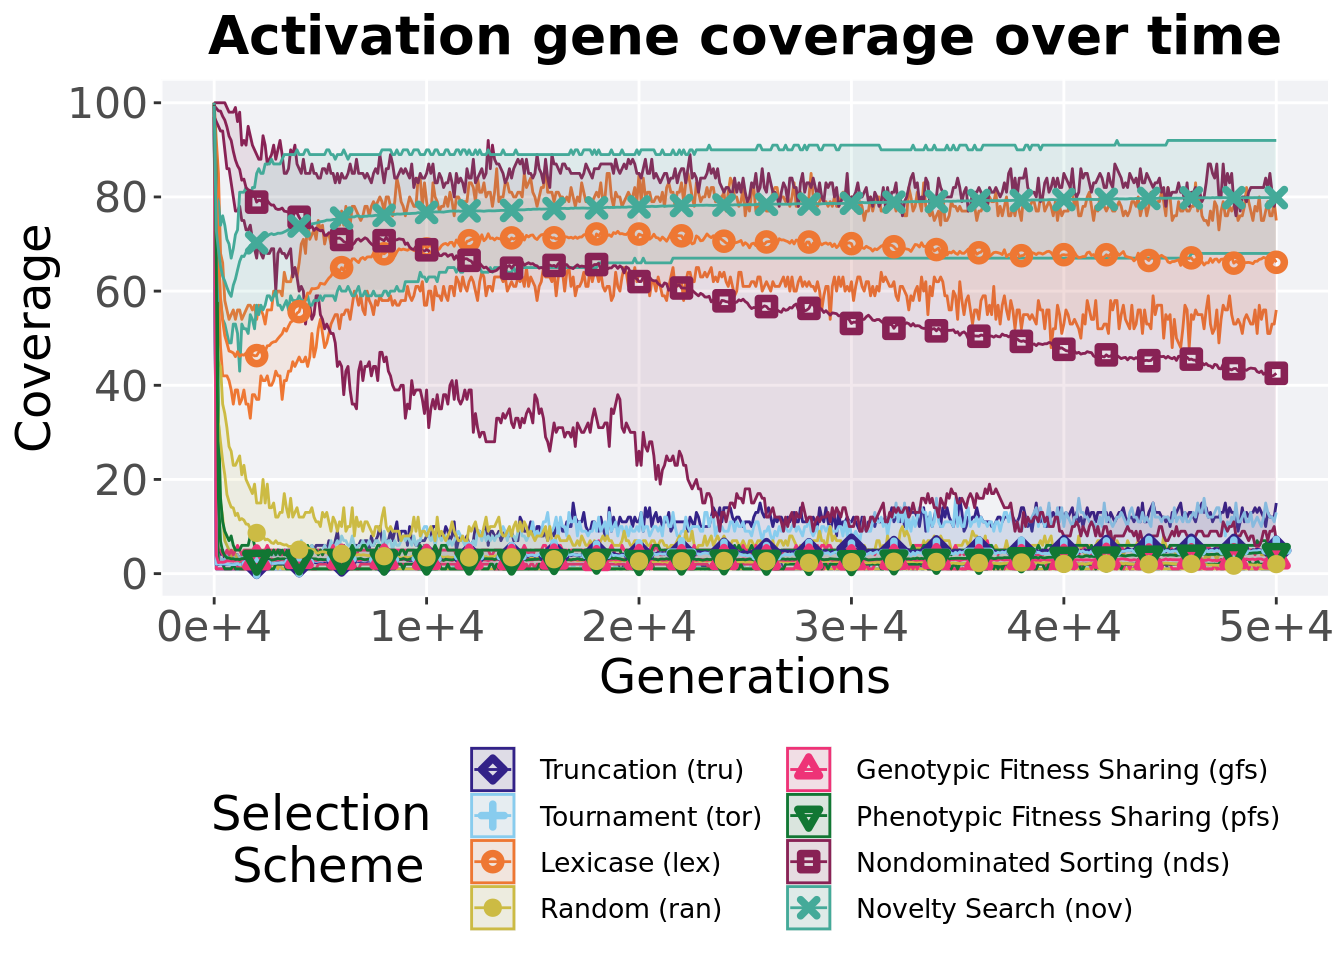
\includegraphics[width=1\linewidth]{base-diagnostics_files/figure-latex/mul-act-ot-1}

\hypertarget{final-activation-gene-coverage-1}{%
\section{Final activation gene coverage}\label{final-activation-gene-coverage-1}}

Activation gene coverage found in the final population at 50,000 generations.

\begin{Shaded}
\begin{Highlighting}[]
\NormalTok{plot =}\StringTok{ }\KeywordTok{filter}\NormalTok{(over_time_df, gen }\OperatorTok{==}\StringTok{ }\DecValTok{50000}\NormalTok{) }\OperatorTok
\StringTok{  }\KeywordTok{ggplot}\NormalTok{(., }\KeywordTok{aes}\NormalTok{(}\DataTypeTok{x =}\NormalTok{ acro, }\DataTypeTok{y =}\NormalTok{ uni_str_pos, }\DataTypeTok{color =}\NormalTok{ acro, }\DataTypeTok{fill =}\NormalTok{ acro, }\DataTypeTok{shape =}\NormalTok{ acro)) }\OperatorTok{+}
\StringTok{  }\KeywordTok{geom_flat_violin}\NormalTok{(}\DataTypeTok{position =} \KeywordTok{position_nudge}\NormalTok{(}\DataTypeTok{x =} \FloatTok{.1}\NormalTok{, }\DataTypeTok{y =} \DecValTok{0}\NormalTok{), }\DataTypeTok{scale =} \StringTok{'width'}\NormalTok{, }\DataTypeTok{alpha =} \FloatTok{0.2}\NormalTok{, }\DataTypeTok{width =} \FloatTok{1.5}\NormalTok{) }\OperatorTok{+}
\StringTok{  }\KeywordTok{geom_boxplot}\NormalTok{(}\DataTypeTok{color =} \StringTok{'black'}\NormalTok{, }\DataTypeTok{width =} \FloatTok{.07}\NormalTok{, }\DataTypeTok{outlier.shape =} \OtherTok{NA}\NormalTok{, }\DataTypeTok{alpha =} \FloatTok{0.0}\NormalTok{, }\DataTypeTok{size =} \FloatTok{1.0}\NormalTok{, }\DataTypeTok{position =} \KeywordTok{position_nudge}\NormalTok{(}\DataTypeTok{x =} \FloatTok{.16}\NormalTok{, }\DataTypeTok{y =} \DecValTok{0}\NormalTok{)) }\OperatorTok{+}
\StringTok{  }\KeywordTok{geom_point}\NormalTok{(}\DataTypeTok{position =} \KeywordTok{position_jitter}\NormalTok{(}\DataTypeTok{width =} \FloatTok{0.03}\NormalTok{, }\DataTypeTok{height =} \FloatTok{0.02}\NormalTok{), }\DataTypeTok{size =} \FloatTok{2.0}\NormalTok{, }\DataTypeTok{alpha =} \FloatTok{1.0}\NormalTok{) }\OperatorTok{+}
\StringTok{  }\KeywordTok{scale_y_continuous}\NormalTok{(}
    \DataTypeTok{name=}\StringTok{"Coverage"}\NormalTok{,}
    \DataTypeTok{limits=}\KeywordTok{c}\NormalTok{(}\DecValTok{0}\NormalTok{, }\DecValTok{100}\NormalTok{),}
    \DataTypeTok{breaks=}\KeywordTok{seq}\NormalTok{(}\DecValTok{0}\NormalTok{,}\DecValTok{100}\NormalTok{, }\DecValTok{20}\NormalTok{),}
    \DataTypeTok{labels=}\KeywordTok{c}\NormalTok{(}\StringTok{"0"}\NormalTok{, }\StringTok{"20"}\NormalTok{, }\StringTok{"40"}\NormalTok{, }\StringTok{"60"}\NormalTok{, }\StringTok{"80"}\NormalTok{, }\StringTok{"100"}\NormalTok{)}
\NormalTok{  ) }\OperatorTok{+}
\StringTok{  }\KeywordTok{scale_x_discrete}\NormalTok{(}
    \DataTypeTok{name=}\StringTok{"Scheme"}
\NormalTok{  )}\OperatorTok{+}
\StringTok{  }\KeywordTok{scale_shape_manual}\NormalTok{(}\DataTypeTok{values=}\NormalTok{SHAPE)}\OperatorTok{+}
\StringTok{  }\KeywordTok{scale_colour_manual}\NormalTok{(}\DataTypeTok{values =}\NormalTok{ cb_palette, ) }\OperatorTok{+}
\StringTok{  }\KeywordTok{scale_fill_manual}\NormalTok{(}\DataTypeTok{values =}\NormalTok{ cb_palette) }\OperatorTok{+}
\StringTok{  }\KeywordTok{ggtitle}\NormalTok{(}\StringTok{'Final activation gene coverage'}\NormalTok{)}\OperatorTok{+}
\StringTok{  }\NormalTok{p_theme}

\KeywordTok{plot_grid}\NormalTok{(}
\NormalTok{  plot }\OperatorTok{+}
\StringTok{    }\KeywordTok{theme}\NormalTok{(}\DataTypeTok{legend.position=}\StringTok{"none"}\NormalTok{),}
\NormalTok{  legend,}
  \DataTypeTok{nrow=}\DecValTok{2}\NormalTok{,}
  \DataTypeTok{rel_heights =} \KeywordTok{c}\NormalTok{(}\DecValTok{3}\NormalTok{,}\DecValTok{1}\NormalTok{)}
\NormalTok{)}
\end{Highlighting}
\end{Shaded}

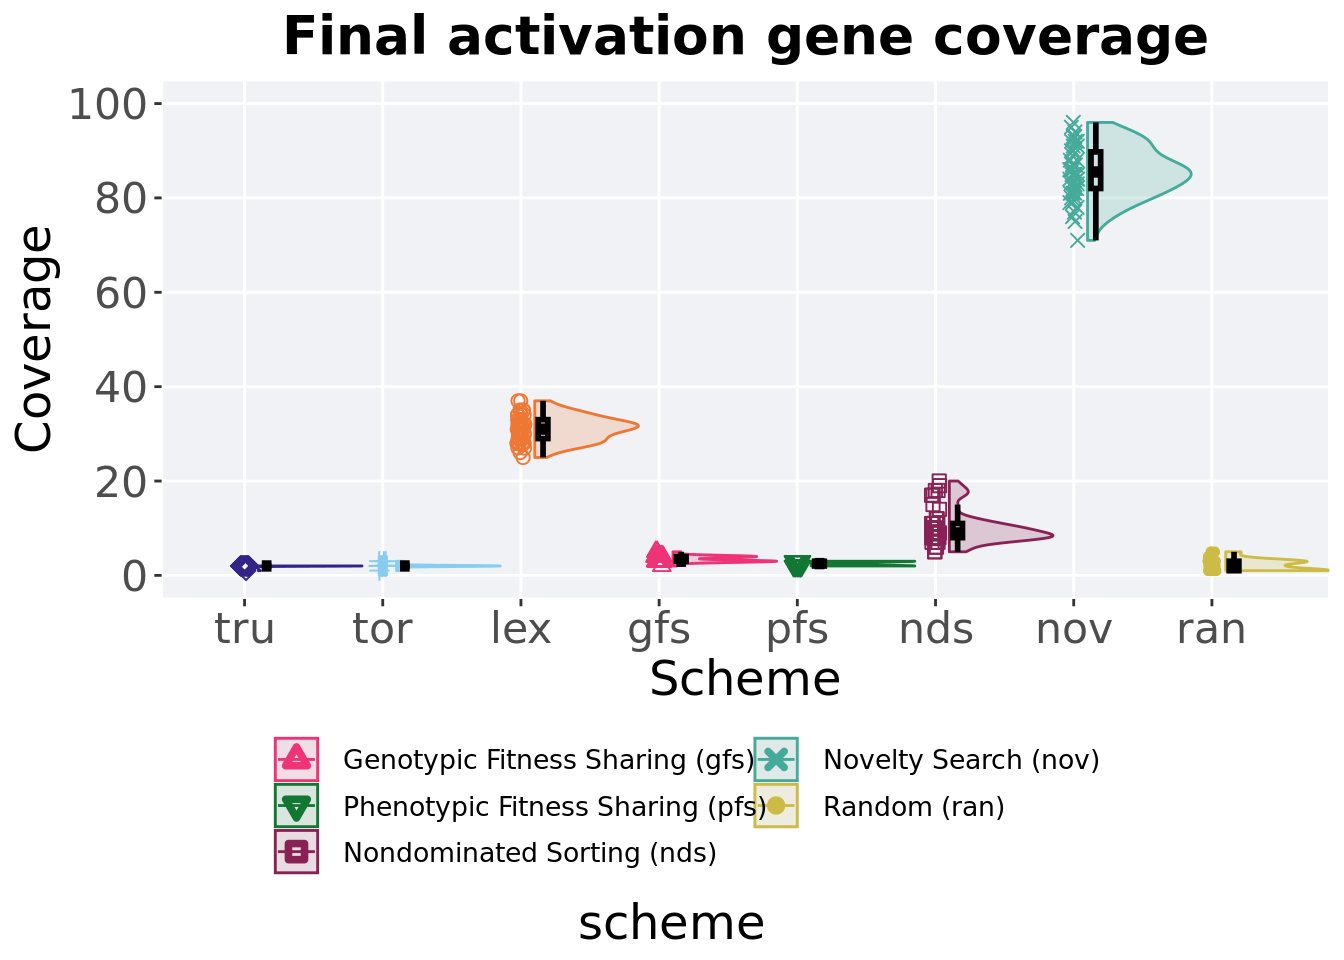
\includegraphics[width=1\linewidth]{base-diagnostics_files/figure-latex/mul-act-end-1}

\hypertarget{stats-7}{%
\subsection{Stats}\label{stats-7}}

Summary statistics for the coverage found in the final population.

\begin{Shaded}
\begin{Highlighting}[]
\NormalTok{act_coverage =}\StringTok{ }\KeywordTok{filter}\NormalTok{(over_time_df, gen }\OperatorTok{==}\StringTok{ }\DecValTok{50000}\NormalTok{)}
\NormalTok{act_coverage}\OperatorTok{$}\NormalTok{acro =}\StringTok{ }\KeywordTok{factor}\NormalTok{(act_coverage}\OperatorTok{$}\NormalTok{acro, }\DataTypeTok{levels =} \KeywordTok{c}\NormalTok{(}\StringTok{'nov'}\NormalTok{,}\StringTok{'lex'}\NormalTok{,}\StringTok{'nds'}\NormalTok{,}\StringTok{'gfs'}\NormalTok{,}\StringTok{'pfs'}\NormalTok{,}\StringTok{'ran'}\NormalTok{,}\StringTok{'tor'}\NormalTok{,}\StringTok{'tru'}\NormalTok{))}
\NormalTok{act_coverage }\OperatorTok
\StringTok{  }\KeywordTok{group_by}\NormalTok{(acro) }\OperatorTok
\StringTok{  }\NormalTok{dplyr}\OperatorTok{::}\KeywordTok{summarise}\NormalTok{(}
    \DataTypeTok{count =} \KeywordTok{n}\NormalTok{(),}
    \DataTypeTok{na_cnt =} \KeywordTok{sum}\NormalTok{(}\KeywordTok{is.na}\NormalTok{(uni_str_pos)),}
    \DataTypeTok{min =} \KeywordTok{min}\NormalTok{(uni_str_pos, }\DataTypeTok{na.rm =} \OtherTok{TRUE}\NormalTok{),}
    \DataTypeTok{median =} \KeywordTok{median}\NormalTok{(uni_str_pos, }\DataTypeTok{na.rm =} \OtherTok{TRUE}\NormalTok{),}
    \DataTypeTok{mean =} \KeywordTok{mean}\NormalTok{(uni_str_pos, }\DataTypeTok{na.rm =} \OtherTok{TRUE}\NormalTok{),}
    \DataTypeTok{max =} \KeywordTok{max}\NormalTok{(uni_str_pos, }\DataTypeTok{na.rm =} \OtherTok{TRUE}\NormalTok{),}
    \DataTypeTok{IQR =} \KeywordTok{IQR}\NormalTok{(uni_str_pos, }\DataTypeTok{na.rm =} \OtherTok{TRUE}\NormalTok{)}
\NormalTok{  )}
\end{Highlighting}
\end{Shaded}

\begin{verbatim}
## # A tibble: 8 x 8
##   acro  count na_cnt   min median  mean   max   IQR
##   <fct> <int>  <int> <int>  <dbl> <dbl> <int> <dbl>
## 1 nov      50      0    71   85.5 85.4     96  7.75
## 2 lex      50      0    25   31   31.1     37  4   
## 3 nds      50      0     5    9   10.2     20  3   
## 4 gfs      50      0     2    3    3.48     5  1   
## 5 pfs      50      0     2    2.5  2.5      3  1   
## 6 ran      50      0     1    2    2.16     5  2   
## 7 tor      50      0     1    2    2.04     3  0   
## 8 tru      50      0     1    2    1.98     2  0
\end{verbatim}

Kruskal--Wallis test illustrates evidence of statistical differences.

\begin{Shaded}
\begin{Highlighting}[]
\KeywordTok{kruskal.test}\NormalTok{(uni_str_pos }\OperatorTok{~}\StringTok{ }\NormalTok{acro, }\DataTypeTok{data =}\NormalTok{ act_coverage)}
\end{Highlighting}
\end{Shaded}

\begin{verbatim}
## 
##  Kruskal-Wallis rank sum test
## 
## data:  uni_str_pos by acro
## Kruskal-Wallis chi-squared = 350.25, df = 7, p-value < 2.2e-16
\end{verbatim}

Results for post-hoc Wilcoxon rank-sum test with a Bonferroni correction.

\begin{Shaded}
\begin{Highlighting}[]
\KeywordTok{pairwise.wilcox.test}\NormalTok{(}\DataTypeTok{x =}\NormalTok{ act_coverage}\OperatorTok{$}\NormalTok{uni_str_pos, }\DataTypeTok{g =}\NormalTok{ act_coverage}\OperatorTok{$}\NormalTok{acro, }\DataTypeTok{p.adjust.method =} \StringTok{"bonferroni"}\NormalTok{,}
                     \DataTypeTok{paired =} \OtherTok{FALSE}\NormalTok{, }\DataTypeTok{conf.int =} \OtherTok{FALSE}\NormalTok{, }\DataTypeTok{alternative =} \StringTok{'l'}\NormalTok{)}
\end{Highlighting}
\end{Shaded}

\begin{verbatim}
## 
##  Pairwise comparisons using Wilcoxon rank sum test with continuity correction 
## 
## data:  act_coverage$uni_str_pos and act_coverage$acro 
## 
##     nov     lex     nds     gfs     pfs     ran tor
## lex < 2e-16 -       -       -       -       -   -  
## nds < 2e-16 < 2e-16 -       -       -       -   -  
## gfs < 2e-16 < 2e-16 < 2e-16 -       -       -   -  
## pfs < 2e-16 < 2e-16 < 2e-16 3.6e-10 -       -   -  
## ran < 2e-16 < 2e-16 < 2e-16 9.4e-08 0.4     -   -  
## tor < 2e-16 < 2e-16 < 2e-16 < 2e-16 1.2e-05 1.0 -  
## tru < 2e-16 < 2e-16 < 2e-16 < 2e-16 1.1e-07 1.0 1.0
## 
## P value adjustment method: bonferroni
\end{verbatim}

\hypertarget{performance-over-time-2}{%
\section{Performance over time}\label{performance-over-time-2}}

Best performance in a population over time.
Data points on the graph is the average performance across 50 replicates every 2000 generations.
Shading comes from the best and worse performance across 50 replicates.

\begin{Shaded}
\begin{Highlighting}[]
\NormalTok{lines =}\StringTok{ }\NormalTok{over_time_df }\OperatorTok
\StringTok{  }\KeywordTok{group_by}\NormalTok{(scheme, gen) }\OperatorTok
\StringTok{  }\NormalTok{dplyr}\OperatorTok{::}\KeywordTok{summarise}\NormalTok{(}
    \DataTypeTok{min =} \KeywordTok{min}\NormalTok{(pop_fit_max) }\OperatorTok{/}\StringTok{ }\NormalTok{DIMENSIONALITY,}
    \DataTypeTok{mean =} \KeywordTok{mean}\NormalTok{(pop_fit_max) }\OperatorTok{/}\StringTok{ }\NormalTok{DIMENSIONALITY,}
    \DataTypeTok{max =} \KeywordTok{max}\NormalTok{(pop_fit_max) }\OperatorTok{/}\StringTok{ }\NormalTok{DIMENSIONALITY}
\NormalTok{  )}
\end{Highlighting}
\end{Shaded}

\begin{verbatim}
## `summarise()` has grouped output by 'scheme'. You can override using the
## `.groups` argument.
\end{verbatim}

\begin{Shaded}
\begin{Highlighting}[]
\NormalTok{lines}\OperatorTok{$}\NormalTok{scheme <-}\StringTok{ }\KeywordTok{factor}\NormalTok{(lines}\OperatorTok{$}\NormalTok{scheme, }\DataTypeTok{levels =} \KeywordTok{c}\NormalTok{(}\StringTok{'Truncation (tru)'}\NormalTok{,}\StringTok{'Tournament (tor)'}\NormalTok{,}\StringTok{'Lexicase (lex)'}\NormalTok{,}\StringTok{'Random (ran)'}\NormalTok{,}\StringTok{'Genotypic Fitness Sharing (gfs)'}\NormalTok{,}\StringTok{'Phenotypic Fitness Sharing (pfs)'}\NormalTok{,}\StringTok{'Nondominated Sorting (nds)'}\NormalTok{,}\StringTok{'Novelty Search (nov)'}\NormalTok{))}

\NormalTok{over_time_plot =}\StringTok{ }\KeywordTok{ggplot}\NormalTok{(lines, }\KeywordTok{aes}\NormalTok{(}\DataTypeTok{x=}\NormalTok{gen, }\DataTypeTok{y=}\NormalTok{mean, }\DataTypeTok{group =}\NormalTok{ scheme, }\DataTypeTok{fill =}\NormalTok{ scheme, }\DataTypeTok{color =}\NormalTok{ scheme, }\DataTypeTok{shape =}\NormalTok{ scheme)) }\OperatorTok{+}
\StringTok{  }\KeywordTok{geom_ribbon}\NormalTok{(}\KeywordTok{aes}\NormalTok{(}\DataTypeTok{ymin =}\NormalTok{ min, }\DataTypeTok{ymax =}\NormalTok{ max), }\DataTypeTok{alpha =} \FloatTok{0.1}\NormalTok{) }\OperatorTok{+}
\StringTok{  }\KeywordTok{geom_line}\NormalTok{(}\DataTypeTok{size =} \FloatTok{0.5}\NormalTok{) }\OperatorTok{+}
\StringTok{  }\KeywordTok{geom_point}\NormalTok{(}\DataTypeTok{data =} \KeywordTok{filter}\NormalTok{(lines, gen }\OperatorTok\StringTok{ }\DecValTok{2000} \OperatorTok{==}\StringTok{ }\DecValTok{0} \OperatorTok{&}\StringTok{ }\NormalTok{gen }\OperatorTok{!=}\StringTok{ }\DecValTok{0}\NormalTok{), }\DataTypeTok{size =} \FloatTok{1.5}\NormalTok{, }\DataTypeTok{stroke =} \FloatTok{2.0}\NormalTok{, }\DataTypeTok{alpha =} \FloatTok{1.0}\NormalTok{) }\OperatorTok{+}
\StringTok{  }\KeywordTok{scale_y_continuous}\NormalTok{(}
    \DataTypeTok{name=}\StringTok{"Average trait score"}\NormalTok{,}
    \DataTypeTok{limits=}\KeywordTok{c}\NormalTok{(}\DecValTok{0}\NormalTok{, }\DecValTok{100}\NormalTok{),}
    \DataTypeTok{breaks=}\KeywordTok{seq}\NormalTok{(}\DecValTok{0}\NormalTok{,}\DecValTok{100}\NormalTok{, }\DecValTok{20}\NormalTok{),}
    \DataTypeTok{labels=}\KeywordTok{c}\NormalTok{(}\StringTok{"0"}\NormalTok{, }\StringTok{"20"}\NormalTok{, }\StringTok{"40"}\NormalTok{, }\StringTok{"60"}\NormalTok{, }\StringTok{"80"}\NormalTok{, }\StringTok{"100"}\NormalTok{)}
\NormalTok{  ) }\OperatorTok{+}
\StringTok{  }\KeywordTok{scale_x_continuous}\NormalTok{(}
    \DataTypeTok{name=}\StringTok{"Generations"}\NormalTok{,}
    \DataTypeTok{limits=}\KeywordTok{c}\NormalTok{(}\DecValTok{0}\NormalTok{, }\DecValTok{50000}\NormalTok{),}
    \DataTypeTok{breaks=}\KeywordTok{c}\NormalTok{(}\DecValTok{0}\NormalTok{, }\DecValTok{10000}\NormalTok{, }\DecValTok{20000}\NormalTok{, }\DecValTok{30000}\NormalTok{, }\DecValTok{40000}\NormalTok{, }\DecValTok{50000}\NormalTok{),}
    \DataTypeTok{labels=}\KeywordTok{c}\NormalTok{(}\StringTok{"0e+4"}\NormalTok{, }\StringTok{"1e+4"}\NormalTok{, }\StringTok{"2e+4"}\NormalTok{, }\StringTok{"3e+4"}\NormalTok{, }\StringTok{"4e+4"}\NormalTok{, }\StringTok{"5e+4"}\NormalTok{)}

\NormalTok{  ) }\OperatorTok{+}
\StringTok{  }\KeywordTok{scale_shape_manual}\NormalTok{(}\DataTypeTok{values=}\KeywordTok{c}\NormalTok{(}\DecValTok{5}\NormalTok{,}\DecValTok{3}\NormalTok{,}\DecValTok{1}\NormalTok{,}\DecValTok{20}\NormalTok{,}\DecValTok{2}\NormalTok{,}\DecValTok{6}\NormalTok{,}\DecValTok{0}\NormalTok{,}\DecValTok{4}\NormalTok{))}\OperatorTok{+}
\StringTok{  }\KeywordTok{scale_colour_manual}\NormalTok{(}\DataTypeTok{values =} \KeywordTok{c}\NormalTok{(}\StringTok{'#332288'}\NormalTok{,}\StringTok{'#88CCEE'}\NormalTok{,}\StringTok{'#EE7733'}\NormalTok{,}\StringTok{'#CCBB44'}\NormalTok{,}\StringTok{'#EE3377'}\NormalTok{,}\StringTok{'#117733'}\NormalTok{,}\StringTok{'#882255'}\NormalTok{,}\StringTok{'#44AA99'}\NormalTok{)) }\OperatorTok{+}
\StringTok{  }\KeywordTok{scale_fill_manual}\NormalTok{(}\DataTypeTok{values =} \KeywordTok{c}\NormalTok{(}\StringTok{'#332288'}\NormalTok{,}\StringTok{'#88CCEE'}\NormalTok{,}\StringTok{'#EE7733'}\NormalTok{,}\StringTok{'#CCBB44'}\NormalTok{,}\StringTok{'#EE3377'}\NormalTok{,}\StringTok{'#117733'}\NormalTok{,}\StringTok{'#882255'}\NormalTok{,}\StringTok{'#44AA99'}\NormalTok{)) }\OperatorTok{+}
\StringTok{  }\KeywordTok{ggtitle}\NormalTok{(}\StringTok{'Performance over time'}\NormalTok{)}\OperatorTok{+}
\StringTok{  }\NormalTok{p_theme }\OperatorTok{+}
\StringTok{  }\KeywordTok{guides}\NormalTok{(}
    \DataTypeTok{shape=}\KeywordTok{guide_legend}\NormalTok{(}\DataTypeTok{ncol=}\DecValTok{2}\NormalTok{, }\DataTypeTok{title.position =} \StringTok{"left"}\NormalTok{, }\DataTypeTok{title =} \StringTok{'Selection }\CharTok{\textbackslash{}n}\StringTok{Scheme'}\NormalTok{),}
    \DataTypeTok{color=}\KeywordTok{guide_legend}\NormalTok{(}\DataTypeTok{ncol=}\DecValTok{2}\NormalTok{, }\DataTypeTok{title.position =} \StringTok{"left"}\NormalTok{, }\DataTypeTok{title =} \StringTok{'Selection }\CharTok{\textbackslash{}n}\StringTok{Scheme'}\NormalTok{),}
    \DataTypeTok{fill=}\KeywordTok{guide_legend}\NormalTok{(}\DataTypeTok{ncol=}\DecValTok{2}\NormalTok{, }\DataTypeTok{title.position =} \StringTok{"left"}\NormalTok{, }\DataTypeTok{title =} \StringTok{'Selection }\CharTok{\textbackslash{}n}\StringTok{Scheme'}\NormalTok{)}
\NormalTok{  )}

\NormalTok{over_time_plot}
\end{Highlighting}
\end{Shaded}

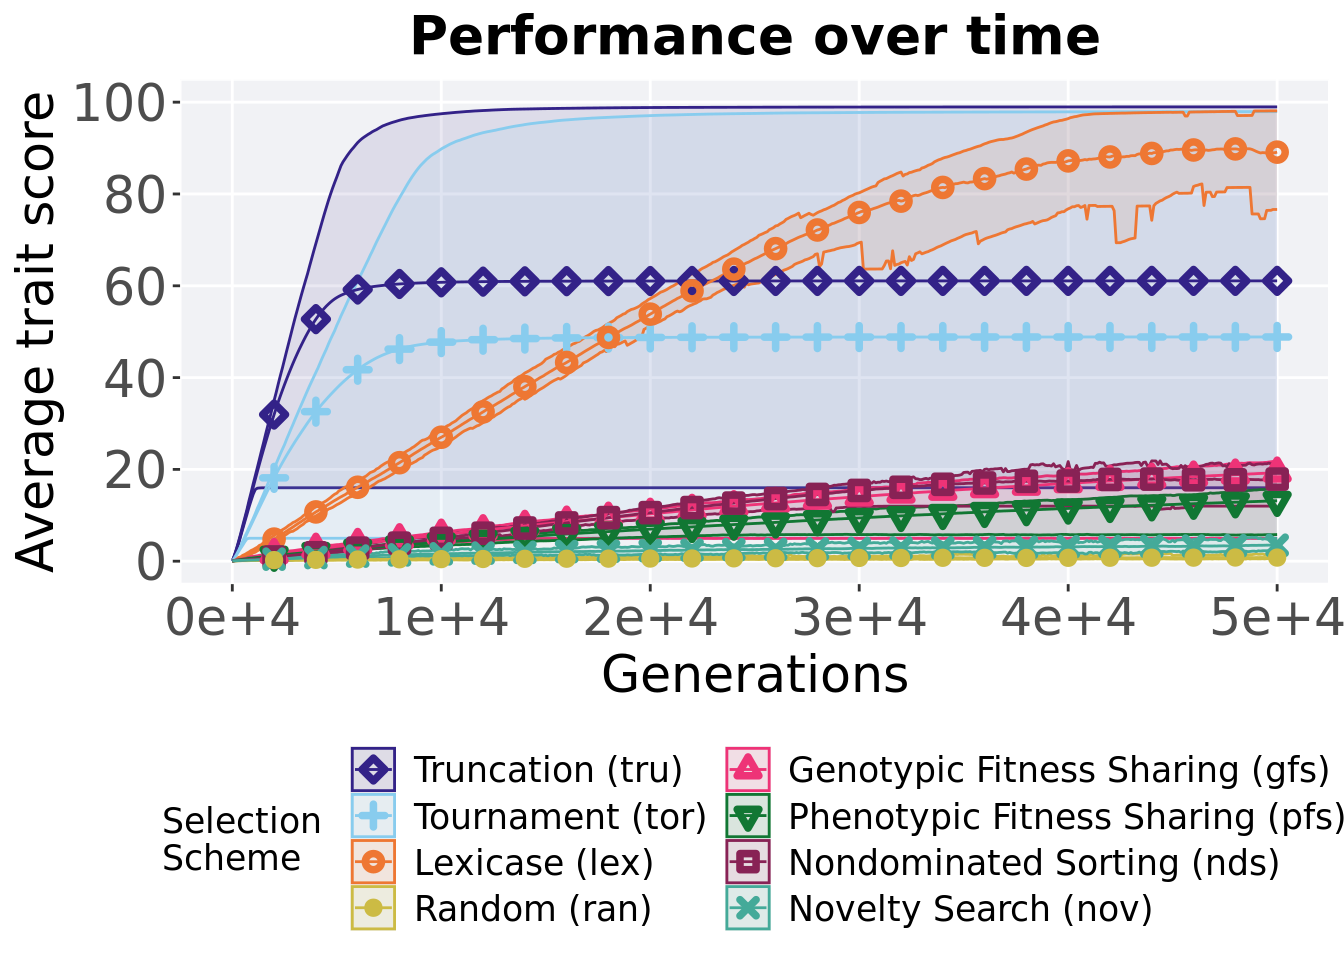
\includegraphics[width=1\linewidth]{base-diagnostics_files/figure-latex/mul-per-ot-1}

\hypertarget{best-performance-throughout-2}{%
\section{Best performance throughout}\label{best-performance-throughout-2}}

Best performance reached throughout 50,000 generations in a population.

\begin{Shaded}
\begin{Highlighting}[]
\NormalTok{plot =}\StringTok{ }\KeywordTok{filter}\NormalTok{(best_df, var }\OperatorTok{==}\StringTok{ 'pop_fit_max'}\NormalTok{) }\OperatorTok
\StringTok{  }\KeywordTok{ggplot}\NormalTok{(., }\KeywordTok{aes}\NormalTok{(}\DataTypeTok{x =}\NormalTok{ acro, }\DataTypeTok{y =}\NormalTok{ val }\OperatorTok{/}\StringTok{ }\NormalTok{DIMENSIONALITY, }\DataTypeTok{color =}\NormalTok{ acro, }\DataTypeTok{fill =}\NormalTok{ acro, }\DataTypeTok{shape =}\NormalTok{ acro)) }\OperatorTok{+}
\StringTok{  }\KeywordTok{geom_flat_violin}\NormalTok{(}\DataTypeTok{position =} \KeywordTok{position_nudge}\NormalTok{(}\DataTypeTok{x =} \FloatTok{.1}\NormalTok{, }\DataTypeTok{y =} \DecValTok{0}\NormalTok{), }\DataTypeTok{scale =} \StringTok{'width'}\NormalTok{, }\DataTypeTok{alpha =} \FloatTok{0.2}\NormalTok{, }\DataTypeTok{width =} \FloatTok{1.5}\NormalTok{) }\OperatorTok{+}
\StringTok{  }\KeywordTok{geom_boxplot}\NormalTok{(}\DataTypeTok{color =} \StringTok{'black'}\NormalTok{, }\DataTypeTok{width =} \FloatTok{.07}\NormalTok{, }\DataTypeTok{outlier.shape =} \OtherTok{NA}\NormalTok{, }\DataTypeTok{alpha =} \FloatTok{0.0}\NormalTok{, }\DataTypeTok{size =} \FloatTok{1.0}\NormalTok{, }\DataTypeTok{position =} \KeywordTok{position_nudge}\NormalTok{(}\DataTypeTok{x =} \FloatTok{.16}\NormalTok{, }\DataTypeTok{y =} \DecValTok{0}\NormalTok{)) }\OperatorTok{+}
\StringTok{  }\KeywordTok{geom_point}\NormalTok{(}\DataTypeTok{position =} \KeywordTok{position_jitter}\NormalTok{(}\DataTypeTok{width =} \FloatTok{0.03}\NormalTok{, }\DataTypeTok{height =} \FloatTok{0.02}\NormalTok{), }\DataTypeTok{size =} \FloatTok{2.0}\NormalTok{, }\DataTypeTok{alpha =} \FloatTok{1.0}\NormalTok{) }\OperatorTok{+}
\StringTok{  }\KeywordTok{scale_y_continuous}\NormalTok{(}
    \DataTypeTok{name=}\StringTok{"Average trait score"}\NormalTok{,}
    \DataTypeTok{limits=}\KeywordTok{c}\NormalTok{(}\DecValTok{0}\NormalTok{, }\DecValTok{100}\NormalTok{),}
    \DataTypeTok{breaks=}\KeywordTok{seq}\NormalTok{(}\DecValTok{0}\NormalTok{,}\DecValTok{100}\NormalTok{, }\DecValTok{20}\NormalTok{),}
    \DataTypeTok{labels=}\KeywordTok{c}\NormalTok{(}\StringTok{"0"}\NormalTok{, }\StringTok{"20"}\NormalTok{, }\StringTok{"40"}\NormalTok{, }\StringTok{"60"}\NormalTok{, }\StringTok{"80"}\NormalTok{, }\StringTok{"100"}\NormalTok{)}
\NormalTok{  ) }\OperatorTok{+}
\StringTok{  }\KeywordTok{scale_x_discrete}\NormalTok{(}
    \DataTypeTok{name=}\StringTok{"Scheme"}
\NormalTok{  )}\OperatorTok{+}
\StringTok{  }\KeywordTok{scale_shape_manual}\NormalTok{(}\DataTypeTok{values=}\NormalTok{SHAPE)}\OperatorTok{+}
\StringTok{  }\KeywordTok{scale_colour_manual}\NormalTok{(}\DataTypeTok{values =}\NormalTok{ cb_palette, ) }\OperatorTok{+}
\StringTok{  }\KeywordTok{scale_fill_manual}\NormalTok{(}\DataTypeTok{values =}\NormalTok{ cb_palette) }\OperatorTok{+}
\StringTok{  }\KeywordTok{ggtitle}\NormalTok{(}\StringTok{'Best performance throughout'}\NormalTok{)}\OperatorTok{+}
\StringTok{  }\NormalTok{p_theme}

\KeywordTok{plot_grid}\NormalTok{(}
\NormalTok{  plot }\OperatorTok{+}
\StringTok{    }\KeywordTok{theme}\NormalTok{(}\DataTypeTok{legend.position=}\StringTok{"none"}\NormalTok{),}
\NormalTok{  legend,}
  \DataTypeTok{nrow=}\DecValTok{2}\NormalTok{,}
  \DataTypeTok{rel_heights =} \KeywordTok{c}\NormalTok{(}\DecValTok{3}\NormalTok{,}\DecValTok{1}\NormalTok{)}
\NormalTok{)}
\end{Highlighting}
\end{Shaded}

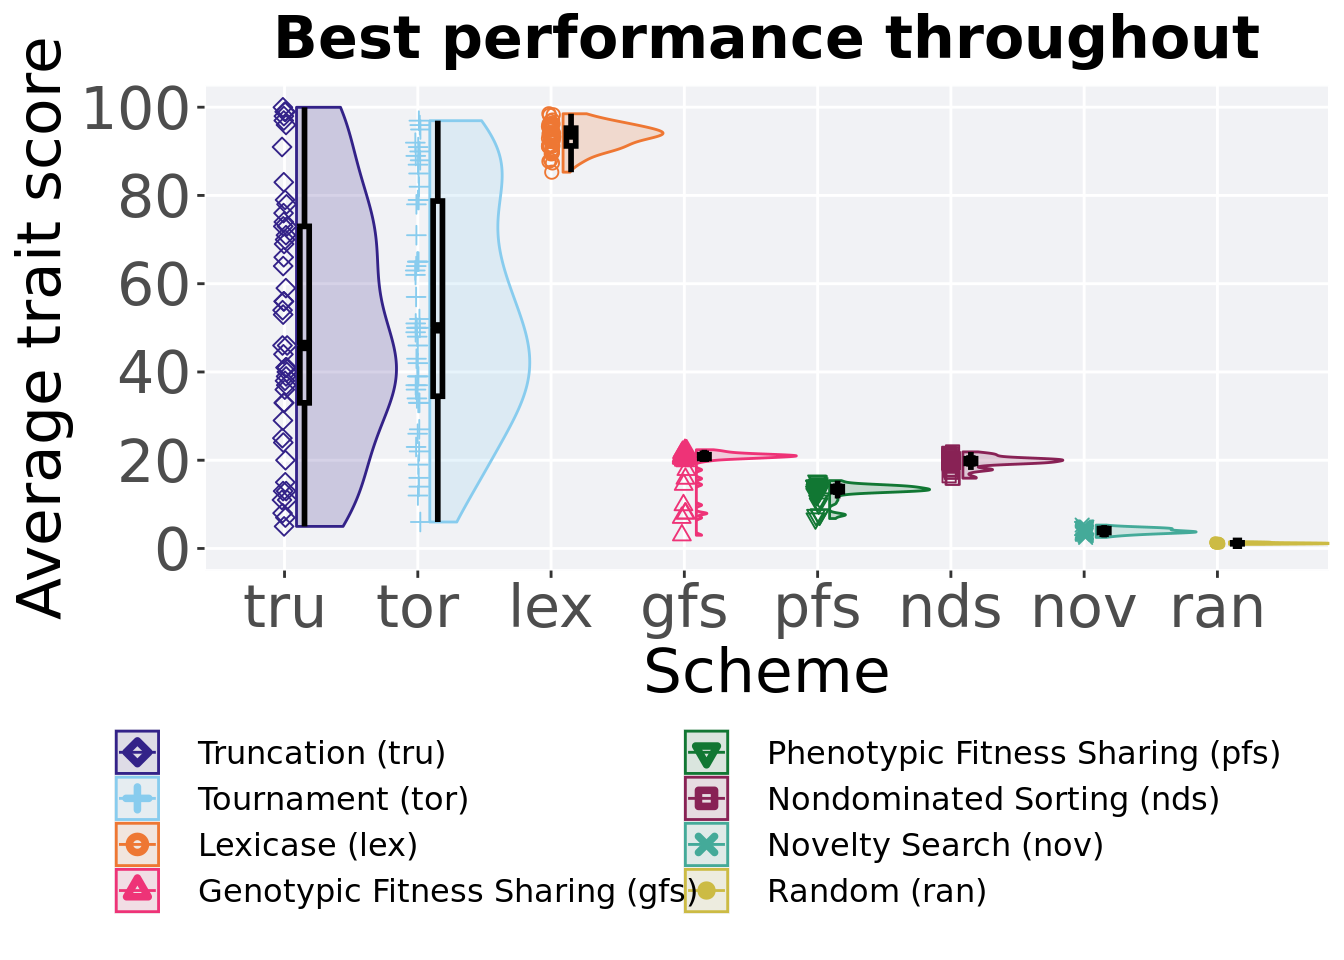
\includegraphics[width=1\linewidth]{base-diagnostics_files/figure-latex/mul-per-bst-1}

\hypertarget{stats-8}{%
\subsection{Stats}\label{stats-8}}

Summary statistics for the best performance.

\begin{Shaded}
\begin{Highlighting}[]
\NormalTok{performance =}\StringTok{ }\KeywordTok{filter}\NormalTok{(best_df, var }\OperatorTok{==}\StringTok{ 'pop_fit_max'}\NormalTok{)}
\NormalTok{performance}\OperatorTok{$}\NormalTok{acro =}\StringTok{ }\KeywordTok{factor}\NormalTok{(performance}\OperatorTok{$}\NormalTok{acro, }\DataTypeTok{levels =} \KeywordTok{c}\NormalTok{(}\StringTok{'lex'}\NormalTok{,}\StringTok{'tru'}\NormalTok{,}\StringTok{'tor'}\NormalTok{,}\StringTok{'gfs'}\NormalTok{,}\StringTok{'nds'}\NormalTok{,}\StringTok{'pfs'}\NormalTok{,}\StringTok{'nov'}\NormalTok{,}\StringTok{'ran'}\NormalTok{))}
\NormalTok{performance }\OperatorTok
\StringTok{  }\KeywordTok{group_by}\NormalTok{(acro) }\OperatorTok
\StringTok{  }\NormalTok{dplyr}\OperatorTok{::}\KeywordTok{summarise}\NormalTok{(}
    \DataTypeTok{count =} \KeywordTok{n}\NormalTok{(),}
    \DataTypeTok{na_cnt =} \KeywordTok{sum}\NormalTok{(}\KeywordTok{is.na}\NormalTok{(val)),}
    \DataTypeTok{min =} \KeywordTok{min}\NormalTok{(val }\OperatorTok{/}\StringTok{ }\NormalTok{DIMENSIONALITY, }\DataTypeTok{na.rm =} \OtherTok{TRUE}\NormalTok{),}
    \DataTypeTok{median =} \KeywordTok{median}\NormalTok{(val }\OperatorTok{/}\StringTok{ }\NormalTok{DIMENSIONALITY, }\DataTypeTok{na.rm =} \OtherTok{TRUE}\NormalTok{),}
    \DataTypeTok{mean =} \KeywordTok{mean}\NormalTok{(val }\OperatorTok{/}\StringTok{ }\NormalTok{DIMENSIONALITY, }\DataTypeTok{na.rm =} \OtherTok{TRUE}\NormalTok{),}
    \DataTypeTok{max =} \KeywordTok{max}\NormalTok{(val }\OperatorTok{/}\StringTok{ }\NormalTok{DIMENSIONALITY, }\DataTypeTok{na.rm =} \OtherTok{TRUE}\NormalTok{),}
    \DataTypeTok{IQR =} \KeywordTok{IQR}\NormalTok{(val }\OperatorTok{/}\StringTok{ }\NormalTok{DIMENSIONALITY, }\DataTypeTok{na.rm =} \OtherTok{TRUE}\NormalTok{)}
\NormalTok{  )}
\end{Highlighting}
\end{Shaded}

\begin{verbatim}
## # A tibble: 8 x 8
##   acro  count na_cnt    min median  mean   max    IQR
##   <fct> <int>  <int>  <dbl>  <dbl> <dbl> <dbl>  <dbl>
## 1 lex      50      0 83.4    92.3  91.9  98.1   5.51 
## 2 tru      50      0 16      66.0  61.1  99.0  47.0  
## 3 tor      50      0  5      47.0  48.9  97.9  46.2  
## 4 gfs      50      0  4.99   20.7  19.3  21.7   1.45 
## 5 nds      50      0 12.0    19.9  19.7  22.8   1.72 
## 6 pfs      50      0  5.87   13.6  13.2  15.9   1.39 
## 7 nov      50      0  2.52    3.83  3.87  5.33  0.793
## 8 ran      50      0  0.865   1.19  1.23  1.72  0.247
\end{verbatim}

Kruskal--Wallis test illustrates evidence of statistical differences.

\begin{Shaded}
\begin{Highlighting}[]
\KeywordTok{kruskal.test}\NormalTok{(val }\OperatorTok{~}\StringTok{ }\NormalTok{acro, }\DataTypeTok{data =}\NormalTok{ performance)}
\end{Highlighting}
\end{Shaded}

\begin{verbatim}
## 
##  Kruskal-Wallis rank sum test
## 
## data:  val by acro
## Kruskal-Wallis chi-squared = 356.22, df = 7, p-value < 2.2e-16
\end{verbatim}

Results for post-hoc Wilcoxon rank-sum test with a Bonferroni correction.

\begin{Shaded}
\begin{Highlighting}[]
\KeywordTok{pairwise.wilcox.test}\NormalTok{(}\DataTypeTok{x =}\NormalTok{ performance}\OperatorTok{$}\NormalTok{val, }\DataTypeTok{g =}\NormalTok{ performance}\OperatorTok{$}\NormalTok{acro, }\DataTypeTok{p.adjust.method =} \StringTok{"bonferroni"}\NormalTok{,}
                     \DataTypeTok{paired =} \OtherTok{FALSE}\NormalTok{, }\DataTypeTok{conf.int =} \OtherTok{FALSE}\NormalTok{, }\DataTypeTok{alternative =} \StringTok{'l'}\NormalTok{)}
\end{Highlighting}
\end{Shaded}

\begin{verbatim}
## 
##  Pairwise comparisons using Wilcoxon rank sum test with continuity correction 
## 
## data:  performance$val and performance$acro 
## 
##     lex     tru     tor     gfs     nds     pfs     nov    
## tru 4.4e-09 -       -       -       -       -       -      
## tor 1.1e-12 0.33    -       -       -       -       -      
## gfs < 2e-16 2.3e-13 4.3e-07 -       -       -       -      
## nds < 2e-16 1.2e-13 6.8e-07 0.47    -       -       -      
## pfs < 2e-16 < 2e-16 5.0e-12 2.3e-11 1.3e-15 -       -      
## nov < 2e-16 < 2e-16 < 2e-16 < 2e-16 < 2e-16 < 2e-16 -      
## ran < 2e-16 < 2e-16 < 2e-16 < 2e-16 < 2e-16 < 2e-16 < 2e-16
## 
## P value adjustment method: bonferroni
\end{verbatim}

\end{document}
